\documentclass[12pt,twoside]{report}
%load packages
\usepackage[utf8]{inputenc}
\DeclareUnicodeCharacter{2009}{\,} 
\usepackage[english]{babel}
\usepackage{csquotes}
\usepackage[a4paper,width=150mm,bindingoffset=6mm,top=25mm,bottom=25mm,headheight=15pt]{geometry}
\usepackage{graphicx}
\usepackage{float}
\graphicspath{{/home/ericulrich/Documents/Master/Masterarbeit/LaTeX_thesis/Main/Images/}{/home/ericulrich/Documents/Master/Masterarbeit/LaTeX_thesis/Introduction/Images/}{/home/ericulrich/Documents/Master/Masterarbeit/LaTeX_thesis/Materialsandmethods/Images/}{/home/ericulrich/Documents/Master/Masterarbeit/LaTeX_thesis/Results/Images/}{/home/ericulrich/Documents/Master/Masterarbeit/LaTeX_thesis/Materialsandmethods/Images/}{/home/ericulrich/Documents/Master/Masterarbeit/LaTeX_thesis/Supplementary/Images/}{/home/ericulrich/Documents/Master/Masterarbeit/LaTeX_thesis/Declaration/Images/}}
\usepackage{amsmath}
\usepackage{refcheck}
\usepackage{textgreek}
\usepackage{hyperref}
\usepackage{gensymb}
\usepackage{lmodern,textcomp}
\usepackage{color, colortbl}
\definecolor{LightCyan}{rgb}{0.88,1,1}
\usepackage{texshade}
\usepackage{longtable}
\usepackage{dnaseq}
\usepackage{tabularx}
\usepackage{pdfpages}
\usepackage{multirow}
	\newcolumntype{L}{>{\raggedright\arraybackslash}X}
\usepackage[table,xcdraw]{xcolor}
\usepackage{dirtytalk}


\bibliographystyle{unsrt}

\usepackage{fancyhdr}
\pagestyle{fancy}
\fancyhead{}
\fancyhead[LO,LE]{\leftmark}
%\fancyhead[RO,RE]{\rightmark}
\fancyfoot{}
\fancyfoot[LO,LE]{Eric Ulrich}
\fancyfoot[CO,CE]{\thepage}
\fancyfoot[RO,RE]{University of Basel}




\usepackage[backend=biber,sorting=none,style=numeric,citestyle=numeric]{biblatex}
\usepackage{url}
\setcounter{biburllcpenalty}{7000}
\setcounter{biburlucpenalty}{8000}
\addbibresource{/home/ericulrich/Documents/Master/Masterarbeit/LaTeX_thesis/Main/bibliography.bib}
\begin{document}

\begin{titlepage}
	\begin{center}
		
\includegraphics[width=0.4\textwidth]{logo}\\
		\vspace{1cm}
		\Large
		Faculty of Science \\
		Department Biozentrum\\
		University of Basel\\
		Switzerland\\
		\date{\today}
		\vspace*{1cm}
		
		\Huge
		Master Thesis Molecular Biology \\
		\vspace{2cm}
		\Huge
		\textbf{Experimental evolution and genotypic characterization of ESBL \textit{Escherichia coli}}
		
		\vspace{3cm}
		\begin{minipage}[t]{0.47\textwidth}
			\textnormal{\large{\bf Submitted to:\\}}
			{\large Prof. Dr. Richard Neher\\ Prof. Dr. Dirk Bumann}
		\end{minipage}\hfill\begin{minipage}[t]{0.47\textwidth}\raggedleft
			\textnormal{\large{\bf Submitted by:\\}}
			{\large Eric Ulrich}
		\end{minipage}			
		\vspace{3.5cm}
		\newline 
		\large{\today}

		
		
	\end{center}
\end{titlepage}
\pagenumbering{roman}
\chapter*{Abstract}
%\addcontentsline{toc}{chapter}{Abstract}
In Swiss hospitals infections with extended-spectrum cephalosporin resistant \textit{Escherichia coli} (\textit{E. coli}) are emerging \cite{swiss_hospitals}. Enzymes called extended-spectrum \textbeta-lactamases (ESBL) are able to hydrolyze extended-spectrum cephalosporins. If expressed in \textit{E. coli}, the susceptibility to extended-spectrum cephalosporins is reduced and the strains are called ESBL \textit{E. coli}. Research focused on studying ESBL mediated extended-spectrum cephalosporin resistance, even though other resistance mechanisms possibly affect the resistance level. We studied the evolution of cefepime (an extended-spectrum cephalosporin) resistance in ESBL \textit{E. coli} strains in order to identify new genotypes possibly associated with resistance mechanisms. In order to do so, we studied whole-genome sequencing data from ESBL \textit{E. coli} isolates from patients of the University Hospital of Basel. These isolates evolved resistance to cefepime in patients. A bioinformatic pipeline was developed for analyzing the sequencing data, revealing several single nucleotide polymorphisms (SNPs) in genomes of isolates which evolved resistance.
Additionally, we assembled a device called morbidostat, which we used to experimentally evolve resistance to cefepime in ESBL \textit{E. coli} strains. The morbidostat is an automated culturing device continuously applying high antibiotic pressure to bacterial cultures resulting in resistance evolution. We cultured three ESBL \textit{E. coli} strains in the morbidostat with cefepime which highly increased the resistance level of the strains. Samples of strains taken during morbidostat experiments were deep-sequenced and analyzed with the same bioinformatic pipeline which was applied to patient isolates. Compared to the genomes of the strains before culturing with the morbidostat, several SNPs were identified in the genomes of the strains which evolved resistance. Interestingly, we found SNPs in the same genes in patients isolates and morbidostat samples, strongly suggesting the importance of the SNPs for the resistance mechanisms. In particular, we identified SNPs in genes coding for the porins \textit{ompC}, \textit{ompF} and their regulatory system in patient isolates and morbidostat samples. Furthermore, SNPs in genes coding for the DNA-directed RNA polymerase subunit \textbeta \space and the RNA polymerase sigma factor in patient isolates and morbidostat samples affected the transcription machinery.  
\chapter*{Acknowledgments}
%\addcontentsline{toc}{chapter}{Acknowledgments}
I would like to thank Richard Neher and Dirk Bumann who gave me the opportunity to work on this very interesting project. Next, I would like to thank everyone in Neher's group for the stimulating discussions and for the friendly environment. Special thanks go to Beatrice Claudi for producing the ESBL plasmids and for answering every microbiology-related question that I had. Furthermore, I would like to thank Sandra Söderholm for supporting me so much with this project and for proofreading my thesis. 
Lastly, I would like to thank my family who supported me throughout the whole year and gave me the opportunity to fully focus on this project. 
\tableofcontents
\pagenumbering{arabic}
\chapter{Introduction}

The discovery of penicillin shortly before the Second World War has revolutionized human medicine in the western world by saving the lives of millions of soldiers and civilians \cite{cdc_biggest_2019}. It also made major advances in surgery possible \cite{worldwar_resistance}. Ever since then antibiotics play a very important role in our well established health system and we are depending on those drugs in order to fight bacterial infections.\\
Because of the positive experiences people made with penicillin they quickly started to use this compound in an irresponsible way. This led to a penicillin resistance within 32 years after it's discovery \cite{worldwar_resistance}.
Ever since then it was necessary to repetitively introduce new antibiotics to the market because bacteria evolved resistance against previously developed drugs. Therefor bacteria which are no longer susceptible to antibiotics are nothing new, the response of resistance to antibiotics has its roots as deep as the discovery of antibiotics itself. 

\section{Cause and urgency of antibiotic resistance}
In the last few decades a gap opened between the increased use of antibiotics and the decreased development of new drugs \cite{ventola_antibiotic_2015}.\\
Based on this imbalance antibiotic resistance emerged and nowadays causes a huge problem in the health sector.  
For example 1.6 € billion and 2.5 million additional hospital days were caused by resistant infections just for the European Union per year \cite{europaisches_zentrum_fur_die_pravention_und_die_kontrolle_von_krankheiten_bacterial_2009}. \\
Or it has been shown that methicillin-resistant Staphylococcus aureus kills more Americans each year than HIV/AIDS, Parkinson’s disease, emphysema, and homicide combined \cite{ventola_antibiotic_2015}.

Between 2000 and 2015 defined daily does of antibiotics increased by 65 \% which demonstrates the tremendous increase of antibiotic consumption \cite{klein_reply_2018}.
This huge increase over the last two decades is terrifying since it's common sense that this is pushing antibiotic resistance even further.\\
Surprisingly a big share of antibiotic consumption is unnecessary and irresponsible. Mainly two fields of heavy antibiotic consumption exists and waste of antibiotics take place in both of them.
One field is the health sector where a questionalbe amount of prescriptions happen.
Alone in the US approximately 50 \% of antibiotics are prescribed unnecessarily \cite{sharma_antimicrobial_2011}. This is mainly because of inaccurate identification of pathogens which could be heavily improved by introducing molecular diagnostic techniques such as PCR \cite{ventola_antibiotic_2015}. \\
The other field is the globally operating food industry. It's estimated that in the early 2000s 25-50 \% of all antibiotic consumption has it's source in the food industry \cite{palumbi_humans_2001}. What makes this extremely high use even less understandable is the fact, that most of the antibiotics are used prophylactic and to stimulate growth and not in order to cure sick animals.

Now that we have seen the perspective of consumption of antibiotics, it's time to look at the development site of antibiotics.\\
As seen earlier the global demand of antimicrobials is extremely high, which is why it's surprisingly that the development of antibiotics decreased significantly. For example 19 antibiotics were approved in 1980-1984. In 2010-2014 only six drugs were approved \cite{ventola_antibiotic_2015}. This observation is not biased by the sampling time but is a tendency which is ongoing since the last three decades. \\
The little interest in the pharmaceutical industry is caused by the cycle of fighting newly formed resistance with novel drugs itself. Newly approved antibiotics are usually held in reserve and only prescribed for infections that more established antibiotics can't treat. This policy helps to delay the emergence of resistant strains, but it also limits the investment in return \cite{fair_antibiotics_2014}. Another reason is that other drugs  are used to treat chronic ailments, antibiotics on the other hand are only used for a short time making them a lot less profitable \cite{fair_antibiotics_2014}. 0.5 billion \$ \cite{costs} is the estimated cost of the development for a novel antibiotic. Considering the reasons mentioned above, such development is seen as a very risky investment \cite{fair_antibiotics_2014}.

Because of the increase of consumption and the lack of development of antibiotics several resistant bacterial pathogens established themselves in recent times. 
Among gram-positive bacteria resistant Staphylococcus aureus currently poses the biggest threat \cite{ventola_antibiotic_2015} as mentioned above causing a severe number of deaths. The threat coming from gram-negative pathogens is even more frightening because many emerged multi drug resistance, making it almost impossible to treat infections caused by such pathogens. Common representatives of gram-negative resistant bacteria are Klebsiella pneumoniae, Pseudomonas aeruginosa, Acinetobacter \cite{ventola_antibiotic_2015} and extended spectrum \textbeta-lactamase (ESBL) producing Escherichia coli \cite{fair_antibiotics_2014}.\\
Since those pathogens listed above and others are becoming more frequently resistant to drugs of last resort the WHO published a list of priority pathogens. This list should encourage development of new antibiotics against pathogens published with this list \cite{noauthor_who_nodate}.\\
Understanding how much antibiotics are prescribed unnecessarily and how irresponsible they are used in the food industry, it's quite obvious that one key of managing resistant pathogens is to stop this extensive overuse. In human medicine new guidelines and methodologies have to be developed which help doctors in the decision whether it's necessary or not to prescribe antibiotics. New guidelines also have to be established in the food industry limiting this excessive prophylactic overuse. \\
Furthermore the development of antibiotics has to be pushed ether by governmental founding/rewards or pharmaceutical companies have to come up with new business models, making the development of antibiotics more profitable.
\newpage

\section{Antibiotics and mechanisms of resistance}
During the 21st century different classes of antibiotics were discovered and developed. All of them have in common, that they intend to harm the bacterial pathogen, without harming the patient. This is possible by targeting bacteria specific target sites. Such targets are often involved in the synthesis of molecules which are essential for the bacterial cell. 
For example tetracyclines inhibit bacterial protein synthesis by binding to 30S ribosomal subunit \cite{noauthor_mechanism_nodate}. Other mechanisms are inhibiting bacterial transcription by blocking the process of unwinding of the bacterial DNA (quinilones) or by inhibitting the folic acid metabolism which is targetd by suflonamides \cite{noauthor_fig._nodate}. 
The most common target is cell wall synthesis, since the cell wall is very specific for prokaryotes. \textbeta-lactams, a class of antibiotics to which also penicillin belongs, target mechanisms in cell wall synthesis. They are the most prescribed antibiotics in human medicine. That's also why a lot of resistant bacterial pathogens are resistant against members of this class of antibiotics \cite{noauthor_high_nodate}. Since with this thesis I'm foucins on resistance against \textbeta-lactams with cephalosporins in particular, I only describe the mechanism of action for this class of antibiotics. 

\subsection{Development and mechanism of action of \textbeta-lactams}

\textbeta-lactam antibiotics act by inhibiting the synthesis of the peptidoglycan layer of bacterial cell walls \cite{noauthor_-lactam_2019}. This is a very effective target, since peptidoglycan plays a fundamental role in the cell wall structure. A damaged cell wall leads to bursting of the cell caused by the osmotic pressure from the cytoplasm. This implements that gram-positive bacteria are especially vulnerable to \textbeta-lactams because the peptidoglycan forms the very outer layer of their cell membrane \cite{graevemoore_english:_2008}.\\
In detail the inhibition of peptidoglycan synthesis happens becuase the \textbeta-lactams are analogues of the amino acid D-alanyl-D-alanine \cite{fisher_bacterial_2005}. Those tow amino acids form the terminal residues of the NAM/NAG-peptides which are subunits of the peptioglycan layer \cite{fisher_bacterial_2005}. Those subunits are crosslinked to peptidogylcan by DD-transpeptidases. Now the \textbeta-lactams also bind to the DD-transpeptidases but they heavily inhibit its activity, which means that the NAM/NAG-peptide subunits are no longer crosslinked \cite{fisher_bacterial_2005}. Because \textbeta-lactams bind to those DD-tranpspeptidases those enyzmes are also called penicillin binding proteins, coming from penicillin being the most famous representative of \textbeta-lactams \cite{fisher_bacterial_2005}.

All of the \textbeta-lactams feature the reactive \textbeta-lactam ring, which is a highly strained and reactive cyclic amide. In general five groups of \textbeta-lactams can be classified. Those being penams, penems, carbapenems, monobactams and the cefems \cite{beta-lactam_nodate}. The classification is done by subgrouping their ring system which is responsible for the antimicrobial action \cite{fernandes_-lactams:_2013}. 
Cephalosporins belonging to the cephems are very important because they showed to be very potent and well tolerated by patients thus they are widely used antibiotics \cite{dancer_problem_2001}. Furthermore Cephalosporins can be divided into five generations which is mostly done based on the time-point of development. \\
First-generation cephalosporins are very active against gram-positive cocci but other than cefazolin which is used for surgical propyhlaxis this generation of drugs in not prescribed often anymore \cite{fernandes_-lactams:_2013}. The second generation of cephalosporins are all active against bacteria covered by first-generation drugs, but have extended coverage against gram-negative bacteria \cite{fernandes_-lactams:_2013}. The tendency of enhanced activity against gram-negative bacteria is further visible in third-generation cephalosporins. A common representative of this generation is ceftazidime \cite{klein_third-generation_1995}. Only two beta-lactams are classified under the fourth-generation of cephalosporins, those being cefepime and cefpirome \cite{fernandes_-lactams:_2013}. They were developed because bacterial pathogens started to gain resistance against third generation cephalosporins. 
The newest fifth generation of caphalosporins were explicitly developed to target resistant strains of bacteria but unfortunatley drugs belonging to this generation are ineffective against enterococci bacteria \cite{fernandes_-lactams:_2013} 

Penams are a large group of \textbeta-lactmas that include penicillins which are characterized by a basic bicyclic structure \cite{beta-lactam_nodate}. \\
Unlike penams, monobactams have a momocyclic \textbeta-lactam ring and are only active against gram-necative bacteria \cite{fernandes_-lactams:_2013}. Lastly carbapenems are also belonging to \textbeta-lactams and they have good activity against many gram-negative bacteria \cite{beta-lactam_nodate}.  

\subsection{Resistance mechanisms against \textbeta-lactams}

Because the \textbeta-lactam ring in \textbeta-lactam antibiotics is very reactive several enzymes are expressed in bacteria which are able to hydrolyze the \textbeta-lactam ring \cite{noauthor_beta-lactam_nodate}. This same ring is also involved in binding to the penicillin binding proteins and therefor hydrolyzed \textbeta-lactams are no longer bactericide \cite{noauthor_beta-lactam_nodate}. Those enzymes called \textbeta-lactamases were found before treatment of infections with \textbeta-lactams, because they occurred naturally in bacteria being exposed to bactericides produced from fungi \cite{noauthor_fig._nodateflem}.   

\subsubsection{\textbeta-lactamases}
Nowadays mainly plasmid-mediated \textbeta-lactamases are important because they can be easily transmitted via horizontal gene-transfer \cite{munita_mechanisms_2016}.  
The first plasmid-mediated \textbeta-lactamase in gram-negative bacteria was described in the early 1960s and called \textbeta-lactamase TEM-1 \cite{fernandes_-lactams:_2013}. Because its position on a plasmid and being transposon mediated, TEM-1 was found worldwide only few years later after it's first isolation \cite{fernandes_-lactams:_2013}. TEM-1 was able to cause resistance against \textbeta-lactams of this time.  That's why third-generation cephalosporins such as ceftazidime were developed which can't be hydrolyzed by TEM-1 \cite{fernandes_-lactams:_2013}. Those newly developed extended spectrum cephalosporins where thus heavily used exposing evolutionary formed variants of TEM-1 to selection \cite{fernandes_-lactams:_2013}. This caused further resistance against those newly developed extended cephalosporins \cite{fernandes_-lactams:_2013}. 
Another anciently known \textbeta-lactamase is called SHV-1 which was isolated for the first time in 1974 \cite{kuzin_structure_1999}. It's encoded chromosomally in the majority of isolates of K. pneumoniae but is also plasmid mediated when present in Escherichia Coli \cite{kuzin_structure_1999}. \\
\textbeta-lactamases which are able to hydrolyze extended-spectrum cephalosporins are called extended-spectrum \textbeta-lactamases or ESBLs. 

\subsubsection{Extended spectrum \textbeta-lactamases (ESBLs)}
Next to the TEM and SHV families new \textbeta-lactamases were isolated over the time of the last couple decades. One of them is called CTX-M-1 \textbeta-lactamase which was clinically isolated for the first time in Germany in 1986. It's name comes from the high affinity to cefotaxime \cite{fernandes_-lactams:_2013}. Because it only has a sequence identity of 40 \% compared to TEM or SHV \cite{bradford_extended-spectrum_2001} it got categorized as a new \textbeta-lactamase family. Later on many variants were isolated and the CTX protein family was subdivided into five subgroups, with CTX-M-1 being one of them  \cite{fernandes_-lactams:_2013}.
It's assumend that they evolved from the \textbeta-lactamase precursor AmpC from Klyzvera ascorbata  \cite{bradford_extended-spectrum_2001}. Even though the first CTX-M-1 was isolated in Germany, it's mostly popular in eastern Europe, South America and Japan \cite{bradford_extended-spectrum_2001}. \\
Another \textbeta-lactamase family belonging to the ESBLs is called OXA.
The OXA family was originally created as a phenotypic rather than a genotypic group, based on a specific hydrolysis profile \cite{bradford_extended-spectrum_2001}. Therefor the sequence identity compared to other members of this family is only about 20 \% \cite{bradford_extended-spectrum_2001}. It's name comes from the ability to efficiently hydrolyze oxacillin \cite{bradford_extended-spectrum_2001}.
\label{section:esbls}

\subsection{General resistance mechanisms}
\label{section:resistance_mechanisms}
By hydrolyzing \textbeta-lactams we have seen one strategy of bacterial resistance against antibiotics. There are other more general mechanisms which protect the pathogen form bactericide effects of antibiotics. \\
Another pathway of resistant bacteria is to decrease the antibiotic penetration and to increase efflux. That makes a lot of sense, because many antibiotics have targets which are located intracellularly \cite{munita_mechanisms_2016}. This implies that bacterial pathogens came up with pathways which are making it more difficult for the antibiotic to reach the cytoplasm, or they introduced pathways which actively transport the antibiotic out of the cell. Some compounds such as \textbeta-lactams rely on channels in the membrane of the bacteria called porins, because they are hyrdophylic and therefor can not just pass the lipophylic membrane by diffusion \cite{munita_mechanisms_2016}. This gives the bacteria the opportunity to reduce the numbers of porins or to change their structure \cite{munita_mechanisms_2016}. It's noteworthy that changing permeability is an especially effective strategy for gram-negative bacteria to protect themselves from \textbeta-lactams. That's because the \textbeta-lactams have to cross the outer membrane in order to inhibit the peptidoglycan synthese \cite{munita_mechanisms_2016}. \\
It's much more complicated on the other hand to produce efflux pumps, which actively transport the toxic compoud out of the cell. One of the earliest described efllux pump system are the Tet efflux pumps which are using proton exchange as source of energy \cite{munita_mechanisms_2016}.\\
Another mechanism is changing of the target site. Some antibiotics such as rifampin binds to a very conserved pocked within the RNA polymerase of the bacteria. Now by chromosomal mutations coding for this RNA polymerase the bacteria changed the structure of this pocket and therefor they were no longer susceptible to rifampin \cite{munita_mechanisms_2016}.    

\section{An overview of antibiotic resistant pathogens in Switzerland}
\begin{figure}
	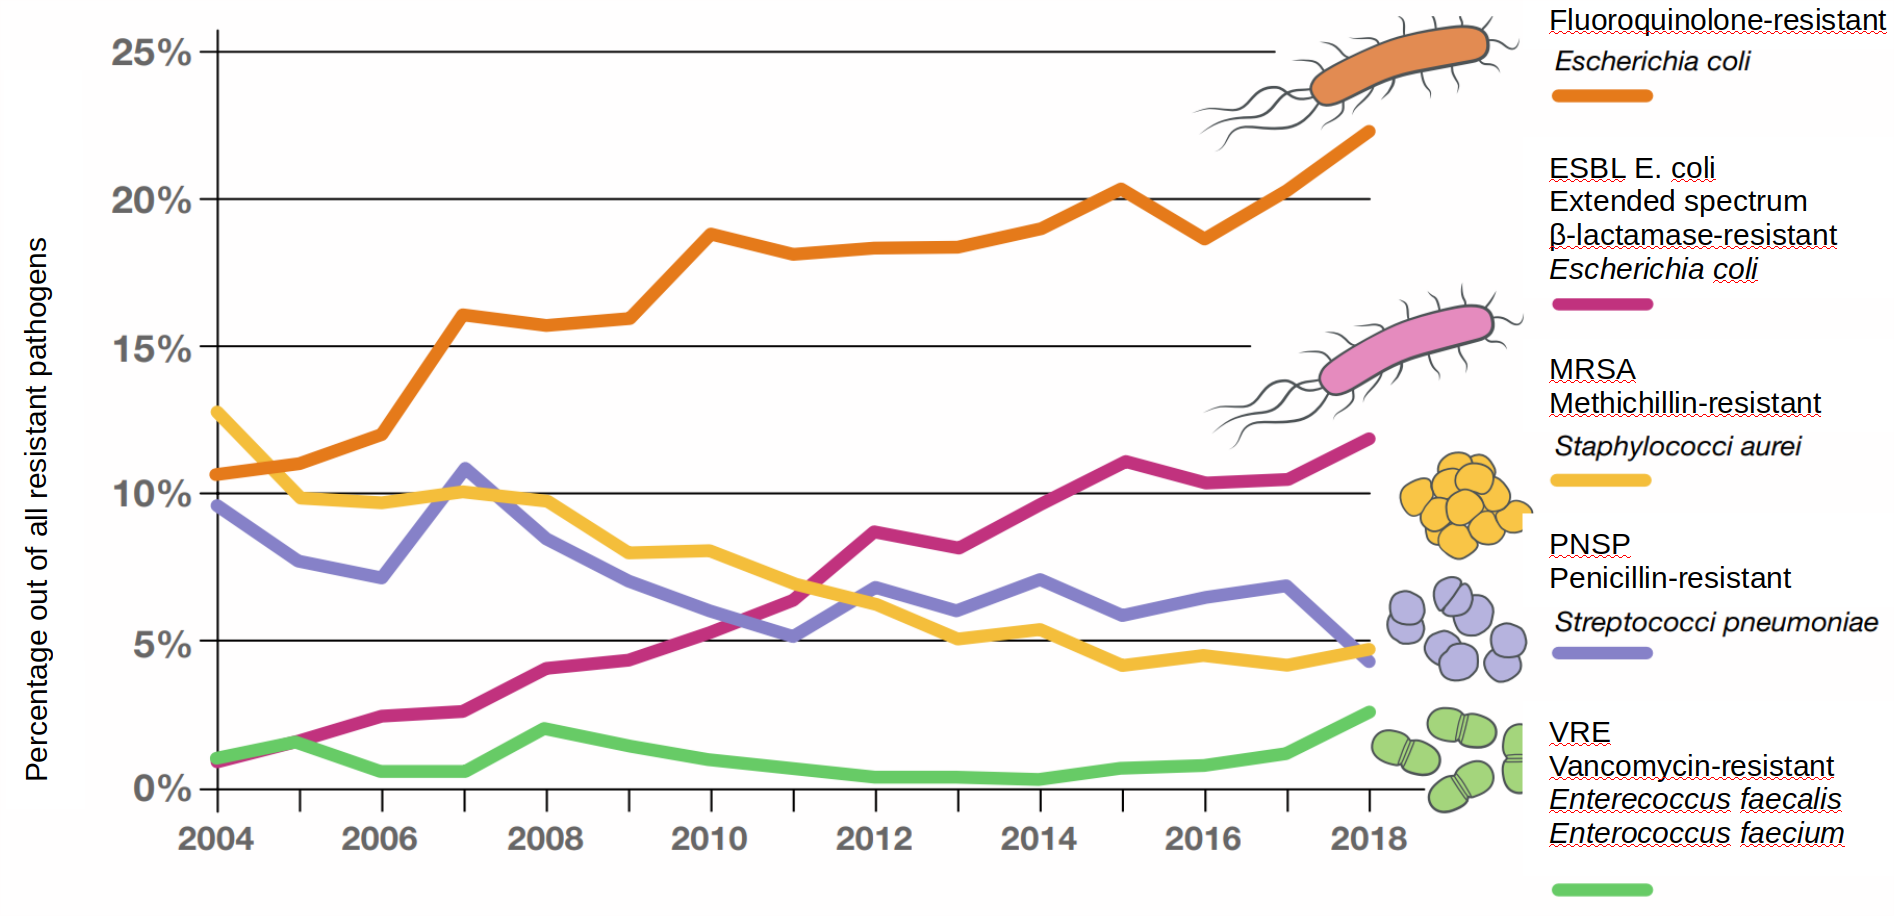
\includegraphics[scale=0.2]{pathogens_overview.png}
	\caption{Development of popularity of antibiotic resistant pathogens.
		\cite{swiss_hospitals_pathogens}}
	\label{figure:pathogen_dvelopment}
\end{figure}

For Switzerland the rate of antibiotic consumption divided by the Swiss population stayed the same in recent times, but the absolute consumption increased too. This is because more people were getting treated in hospitals \cite{swiss_hospitals} but the general population of Switzerland increased too.

The biggest challenge with resistant pathogens in Switzerland is ongoing in hospitals where yearly 300 people die because of infections with antibiotic resistant bacteria \cite{noauthor_fast_2018}. Hospitals are often hot-spots of resistant bacteria because there is a high density of  pathogens, combined with high locally applied antibiotic doses. This generates an increased antibiotic pressure and selection. Unfortunately many patients have a weakened immune system making them a lot more vulnerable to infections with antibiotic resistant bacteria.


Mainly five strains which cause problems in treatment with antibiotics are present in Swiss hospitals. Their increasing or decreasing spread can be seen in Figure \ref{figure:pathogen_dvelopment}\cite{swiss_hospitals}. 

\textbf{Staphylococcus aureus} is a gram-positive bacterium which is normally present in the upper respiratory tract and on the skin. As a pathogen Staphylococcus aureus can cause skin and bone inflammations and is responsible for the most inflammations of surgical wounds \cite{tong_staphylococcus_2015}. The most common resistance formed by S. aureus is resistance against an antibiotic called methicillin, a penicillin like compound. Resistance is achieved by those pathogens by expressing a gene coding for for a penicillin binding protein PBP2a which has significantly lower affinity to \textbeta-lactams \cite{peacock_mechanisms_2015}.  There are compounds which effectively kill this certain pathogen but resistance against such compounds have been reported already \cite{ventola_antibiotic_2015}. As seen in Figure \ref{figure:pathogen_dvelopment} there is a decrease of this pathogen which could mainly be achieved by aggressive preventive hygiene measures in hospitals and improved screening for this pathogen \cite{ventola_antibiotic_2015}\cite{swiss_hospital}. 

\textbf{Streptococcus pneumoniae}, a gram-positive bacteria, is normally present in the nose and throat of most individuals \cite{ventola_antibiotic_2015}. But when Streptococcus pneumoniae turns into a pathogen, which mainly happens in elderly patients, it causes severe blood and pulmonary infection causing around 7000 deaths per year \cite{ventola_antibiotic_2015e}. Usually resistant S. pneumoniae are not susceptible to penicillin like antibiotics by a similar mechanism as described for S. auresus (mutations in the penicillin binding proteins). Visible in Figure \ref{figure:pathogen_dvelopment}, this pathogen is decreasing as well, which is mainly because of the introduction of the PCV7 vaccine. This vaccine provides protection against several pneumococcal strains, which reduces the transmission of resistance \cite{ventola_antibiotic_2015}. 

\textbf{Enterococci} such as Enterococcus faecalis are responsible for a rather small share of resistant pathogens as visible in Figure \ref{figure:pathogen_dvelopment}. Unfortunately it's very difficult to treat this gram-positive bacteria because only very few antimicrobial options are available \cite{ventola_antibiotic_2015}. This pathogen is so hard to treat because it developed several pathways of mechanism. Modifications in penicillin binding proteins, over-expression of efflux pumps and a cell response that promotes survival in the human host \cite{miller_mechanisms_2014}.

\textbf{Escherichia coli} belongs to the enterobacteriaceae and is present in every intestine as a gram-negative bacterium. However they are able to cause infections when present in other parts of the body leading mainly to infections of the urinary tract but also in the brains of new borns \cite{swiss_hospitals_pathogens}. Traditionally treatment of E. coli was successful by applying doses of third-generation cephalosporines. In the last two decades E. coli started to gain resistance against such extended \textbeta-lactams by producing extended spectrum \textbeta-lactamases (also see section \ref{section:esbls}). As seen in Figure \ref{figure:pathogen_dvelopment} in 2004 only 1 \% of of resistant pathogens in Swiss hospitals were ESBL prodcuing E. coli. 14 years later they were already responsible for 14 \% of infections with resistant pathogens. Luckily ESBL producing E. coli are still susceptible to carbapenems but other bacterial strains already developed resistance against carbapenems \cite{noauthor_treatment_nodate}. That's why carbapemen should only be used as a very last option of treatment of ESBL E. coli infections, because chances are quite high, that they are able to evolve resistance against this compound too by for example picking up genes by horizontal gene transfer coding for carbapenemases which are able to hydrolyze crabapenem.  \cite{ventola_antibiotic_2015}. 


\section{ESBL E. coli}
Since by now ESBL E. coli can still be treated with antibiotics of last resort such as carbapenems it's extremly important to use those drugs with high awareness. Therefor institutions such as the EUCAST came up with guidelines in order to assist clinical microbiologist in making the right decision in prescribing adequate antibiotics \cite{leclercq_eucast_2013}. The EUCAST is also responsible for defining breakpoints. This means they publish data defining which concentration has to be exceeded in order that a certain pathogens is seen as resistant against a specific antibiotic \cite{leclercq_eucast_2013}. \\
In the past when it was determined that an infection is caused by E. coli, the strain was cultured and susceptibility was tested by determining the MIC. Additionally presence or absence of an ESBL genes was tested by molecular characterisation \cite{kahlmeter_breakpoints_2008}. Such molecular characterisation was typically done by PCR or microarrays \cite{arlet_molecular_1995}. Now when ether the determined MIC was above the breakpoint defined by the EUCAST or the molecular characterisation showed positive results for ESBLs, carbapenemes were described. But it was shown, that sometimes the MIC was below the breakpoint even though ESBLs were detected. Prescribing antibiotics of last resort in such cases was therefor proven to be unnecessary and wrong. As a reaction EUCAST corrected their guidelines and now just susceptibility by MIC determination is considered for making the decision which antibiotic should be prescribed \cite{leclercq_eucast_2013}. Unfortunately MIC determination takes about 48 hours which is too long in some cases forcing prescription of carbapenemens even though it's unknown if it's actually necessary.\\
Completely ignoring genomic data seams not ideal, because chances are quite high that whether E. coli which have ESBL genes are resistant or not is encoded in the genome. This just means that other characteristics have to be defined, since it's not sufficient to simply look if genes coding for ESBLs are present.

\section{Studying differences in the genome between extended cephalosporine susceptible and resistant E. coli}
Some resistant mechanism as for example a change in the target binding site, rely on mutations and therefore imply a change in the genome. Other examples for resistance based on mutations are a different structure of porins making the membrane less permeable for \textbeta-lactams, or a change in the structure of efflux pumps which may changes the affinity for a certain substrate. Other mechanisms could rely on up-regulation, which could have its source in a mutation in a promoter region. \\
As by now it was assumed that the resistance of ESBL E. coli is based on the expression of ESBLs, which are able to hydrolyze \textbeta-lactams \cite{shaikh_antibiotic_2015}. But as described earlier some E. coli which have ESBL coding genes are not resistant. This could mean that extended cephalosporine susceptible E. coli which have ESBL genes are not actually expressing such \textbeta-lactamases. This could be clarified by studying the ESBL protein levels for susceptible and resistant ESBL E. coli. It's also possible, that other resistant mechanisms other than hydrolysis of the compound have an impact on susceptibility.\\
Ether if a change in the expression levels or other mechanisms are responsible for the resistance, it's quite possible that at least a part of the resistance is based on mutations. Those mutations could be identified by comparing the genomes of susceptible and resistant E. coli. \\
Our goal is to identify such mutations which could be involved in the resistance. In order to do so, we pursue two different approaches. One of them is study the genomes of clinical samples of ESBL E. coli which are provided by our collaborator who is the head of clinical microbiology at the University hospital of Basel. He took samples of patients who were infected with E. coli where ESBLs were detected by PCR. Over the process of treatment he continously took samples and determined their susceptibility to cefepime and ceftazidime. This lead to a sample collecton of ESBL E. coli which were susceptible to extended cephalosporines but evolved resistance, or for some patients resistance was lost over time. By isolating the DNA and deep-sequencing all of the isolates, we identify SNPs in the resistant samples, which are potentially involved in the resistant mechanism. \\
For the other approach we assemble a system called morbidostat, which allows to automatically culture bacteria. The morbidostat is continiously recording the growth of the cultures and injects appropriate doses of antibiotics. This creates constant inhibition of the growth and forces resistance and selection. Along this pathway we want to take samples and deep-sequence the isolated DNA. Similar to analysis for the clinical samples, we want to identify mutations which accumulated over the time where the bacteria were forced to evolve resistance. \\
Both approaches rely on next generation sequecing technologies. 
To get the most accurate genomes we want to use two different next generation sequencing technologies.  

\subsubsection{Illumina and Nanopore sequning}
Illumina sequencing is a method which produces short reads which are typically 150 base pairs (bp) long. The strong-suit of Illumina sequecning is the low error rate which was dertermined as 0.24 \% per base \cite{pfeiffer_systematic_2018}. A common used Illumina sequecing system is the MiSeq-System which is also used for this project. The downside of this technology is that even though sequencing itself is rather cheap, the instrument costs are high. Furthermore Illumina sequecing has a tendency to generate more reads of GC-enriched DNA fragments \cite{noauthor_illumina_nodate}. Also it's not possible to assemble structurally correct whole-genomes, because the reads are short. 

Oxford Nanopore Technologies allows sequencing with very little laboratory equipment which is also coming with very low instrument costs. This technology produces very long reads which are up to several 100 kbp long. In contrast to Illumina sequencing the error rate per base is 13.6 \% \cite{noauthor_resolving_nodate} which is a lot higher. But because the reads are so long it's possible to assemble structurally correct whole-genomes. \\
By comparing both technologies, it's pretty obvious that their strong suits are quite contrary. Illumina produces short but accurate reads, Nanopore long and inaccurate reads. Since the costs of both techniques dropped tremendously over the last couple years, it's possible to sequence DNA isolates on both platforms and combine the output in one assembly which is called hybrid assembly. This has the benefit that the advantages of both platforms are combined, leading to assemblies with a low nucleotide error rate but also with high structural correctness.  \\


\subsection{Principles and experiences with the morbidostat} 
The morbidostat was initially invented by Toprak et al \cite{morb_toprak}. Later on Neher et al \cite{doselmann_rapid_2017} rebuilt the system in 2015. Based on those two systems we rebuild a morbidostat with small modifications which should improve the handling and mainly make it a lot more compact. This is important since we want to use the morbidostat in a space limiting hypoxi-station. \\
With the morbidostat 15 cultures can be grown independently in vials. Thereby the growth of each culture is monitored by measuring and saving the optical density (OD). As shown in the left Figure \ref{figure:vial_setup} measuring of the OD is done by detecting scattered light emitted by LEDs. Based on the growth an appropriate dose of antibiotics is calculated using a control algorithm and injected into the cultures. This leads to an inhibition of the growth without entirely killing ever colony forming unit. The appropriate dose of antibiotics is achieved by mixing different drug concentrations using computer controllable pumps which are also injecting the drug into the vials.
The morbidostat allows to study drug resistance evolution in real-time, while having an idea of the progress of evolution in resistance.

In the morbidostat, bacteria are grown in a fixed volume. The process of suppressing the growth with antibiotics is divided into cycles which are constantly getting executed. One cycle has following tasks and commands:
\begin{itemize}
	\item Measuring the OD every several seconds over a defined cycle time \textDelta t, which is typically 10 minutes 
	\item Calculating growth rate at the end of the cycle based on the previously collected ODs
	\item Based on growth, injection of appropriate dose of drug, as calculated by a feedback algorithm
	\item Remove excess volume (waste)
\end{itemize}
In the right Figure \ref{figure:vial_setup} three cycles are shown. Because under certain conditions fluid is getting injected, this leads to a dilution is visible in the OD at the start of the new cycle. \textDelta OD represents how fast the bacteria are grown. It's the difference of the optical densities from the end of two cycles.  
\begin{figure}
	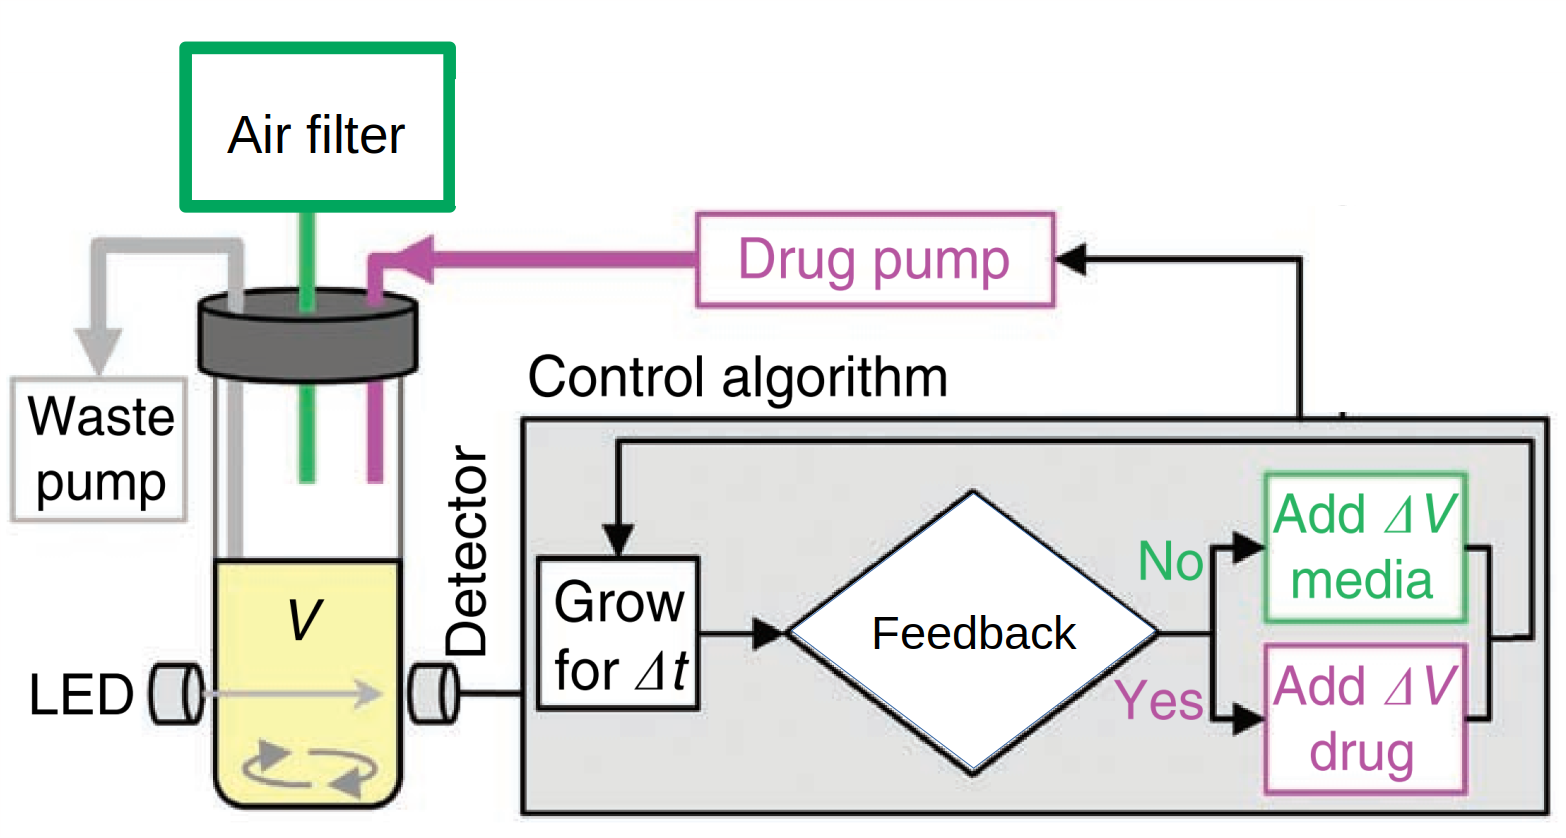
\includegraphics[scale=0.1]{vial_diagram.png}
	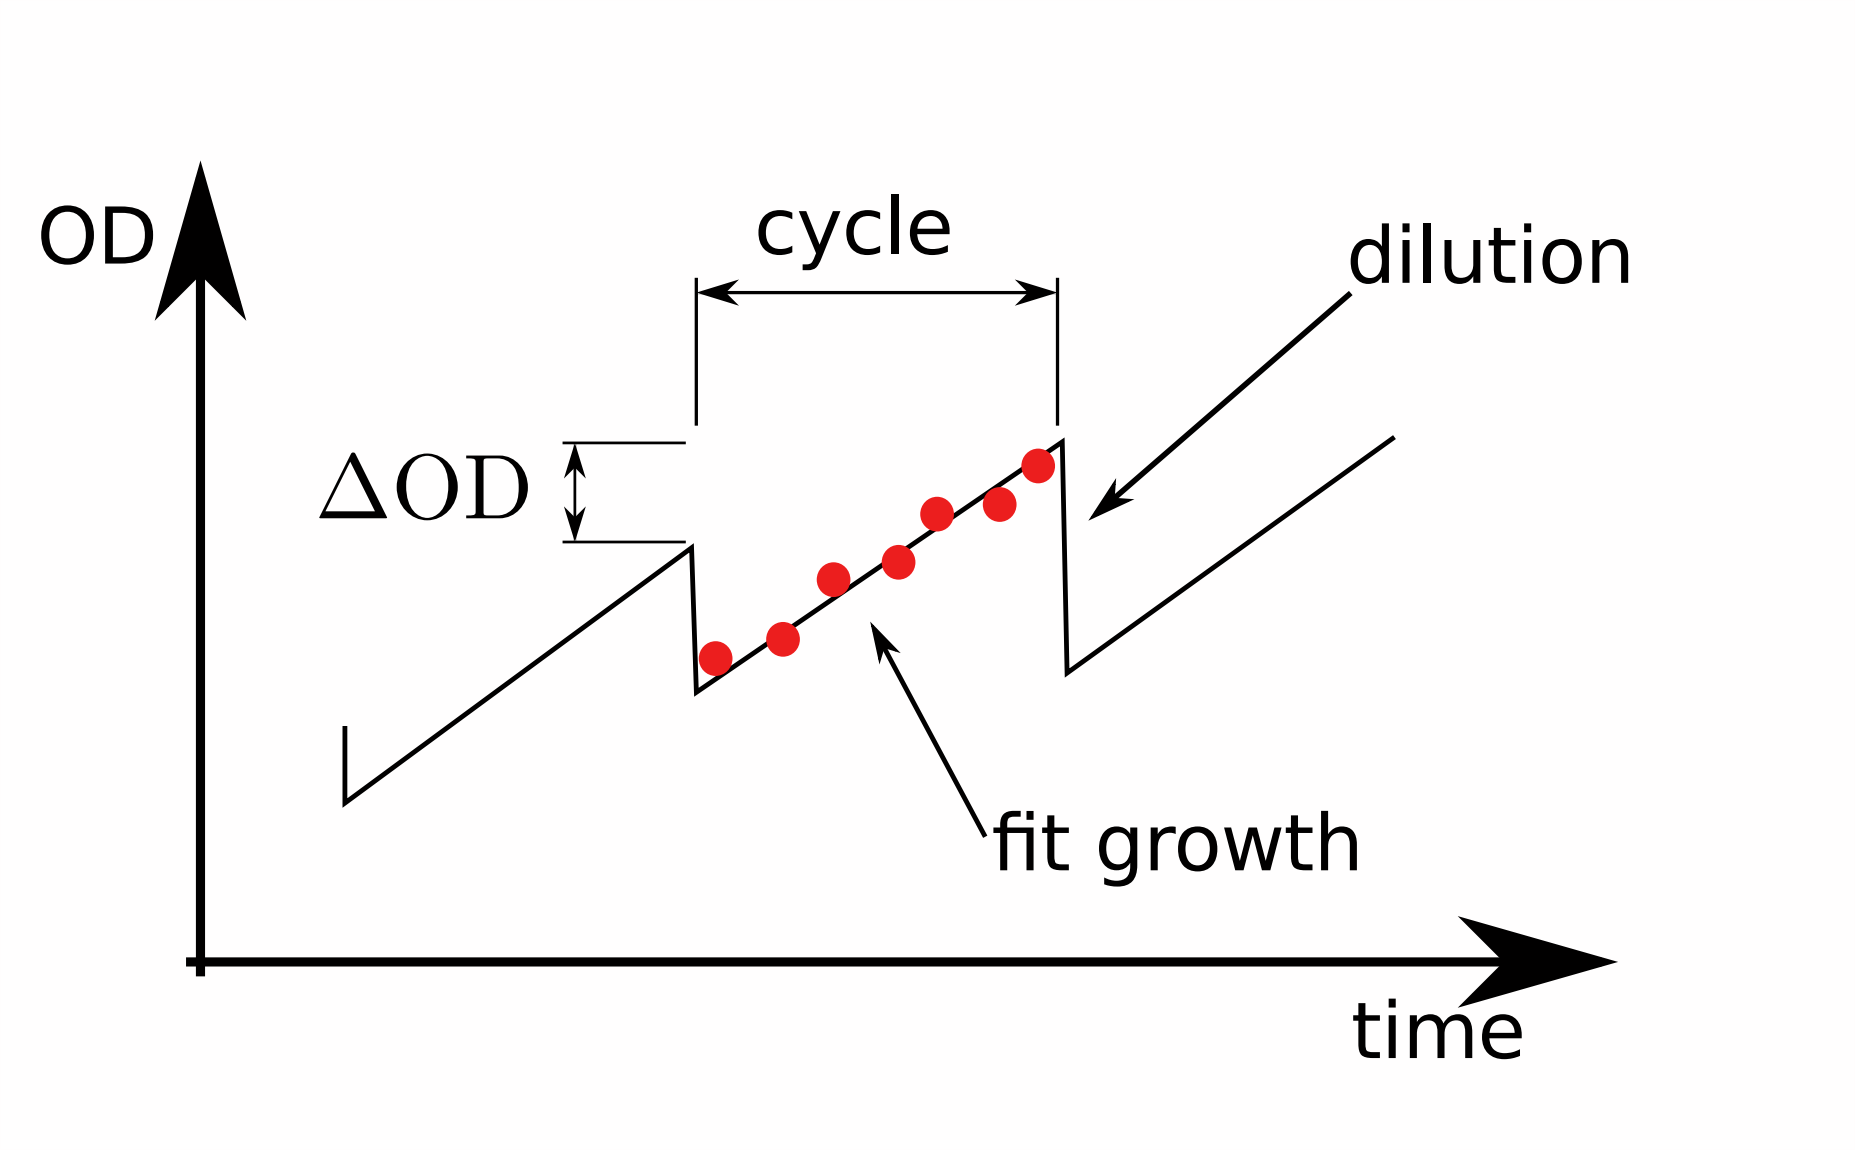
\includegraphics[scale=0.07]{growth_diagram.png}
	\caption{Based on the growth a feedback algorithm decides whether and how much drug is getting injected}
	\label{figure:vial_setup}
\end{figure}

\subsubsection{Previous morbidostat experiments and expected outcome}
Dösselmann et al \cite{doselmann_rapid_2017} used the morbidostat in order to study colistin resistance. With the morbidostat they were able to increase the MIC of colistin for Pseudomanas aeruginosa a 100-fold within 20 days \cite{doselmann_rapid_2017}. Along the evolutionary pathway they were able to identify a mutation pattern. The mechanism of action for colistin is to displace cations from the phospate groups of membrane lipids. This leads to disruption of the outer cell membrane causing cell death \cite{noauthor_colistin:_nodate}. Therefor it's not surprise that Bianca et al could identify several mutations coding fro proteins involved in the lipopolysaccharide synthesis \cite{doselmann_rapid_2017}. 
\\
The mutations that we find in the analysis form the clinical samples but also from the morbidostat experiment hopefully lead to a better understanding in the resistance mechanism of ESBL E. coli. Obviously the data has to be validated by for example  synthetically introducing mutations of interest to extended cephalosporine susceptible ESBL E. \\
The mutations can be used by our collaborator who is studying protein levels in ESBL E. coli. For example mutations found in promotor region can be compared to protein level expression data in order to tell if they have an impact on the expression.

\chapter{Materials and methods}
This work focuses on identifying mutations which accumulated by evolutionary pathways and are potentially involved in the resistance mechanism of ESBL \textit{E. coli} against cefepime. ESBL \textit{E. coli} samples which emerged resistance in patients of the University hospital of Basel were analyzed with a bioinformatical pipeline. Furthermore, we assembled a morbidostat which allowed us to experimentally evolve resistance of ESBL \textit{E. coli} against cefepime. Mutations along this pathway were identified following the same bioinformatical pipe line as for the samples obtained from patients.

\section{ESBL \textit{E. coli} samples from patients at the University Hospital of Basel}
Our collaborators from the clinical microbiology of the University hospital of Basel provided a sample collection of 65 ESBL \textit{E. coli} samples coming from 34 patients. This resulted in ESBL \textit{E. coli} sample series with one to four samples per patient. The sampling period was between 2011 and 2015. Sample collection for one patient typically happened within several months.
\label{section:sample_collection}

\subsection{Screening for ESBLs}
The collected \textit{E. coli} samples were determined as ESBL producing by carrying out combination disc tests. Therefore, they prepared cell suspensions equal to 0.5 McFarland standard. Those suspensions were spread over the entire are of Mueller Hinton agar plates. On those plates disks with ether 30 \textmu g ceftazidime, 30 \textmu g + 10 \textmu g clavulanic acid, 30 \textmu g cefepime and 30 \textmu g cefepime + 10 \textmu g clavulanic acid were applied. All plates were incubated for 20 hours. The inhibition zones caused by the disks were measured. 

\subsection{Selection of samples suitable for our analysis}
Our collaborators determined the MICs of every sample for the third-generation cephalosporin ceftazidime and the fourth-generation cephalosporin cefepime. The MICs were determined by performing E tests. From an agar plate a few colonies were picked and diluted to 0.5 McFarland with physiological NaCl-solution. The suspension was plated on an agar plate. A reagent strip with ether a ceftazidime or cefepime gradient was placed in the middle of the plate. After 22 hours the resulting minimal inhibitory concentration was checked. 
Some sample series showed a significant change of the MICs. Sometimes resistance was gained, but in certain cases resistance was also lost. We were interested in identifying mutations in sample series where susceptibility significantly changed and all the samples from a series were the same ESBL \textit{E. coli} strain.
\label{section:samples}

\subsection{Pylogenetic analysis}
We checked if samples of a series were all the same ESBL \textit{E. coli} strain by running a phylogenetic analysis with Illumina sequencing data from the samples. For the phylogenic analysis we used a tool called PanX \cite{ding_panx:_2018}. Illumina data for every sample was provided by our collaborator (see Section \ref{section:illumina}) .

\subsubsection{PanX}
PanX is a tool which clusters genes into orthologous clusters. From those clusters, panX identifies the core genome which are genes shared by all samples in the cluster. Based on those core genomes a strain-level phylogeny is build, making use of single nucleotide polymorph positions (SNPs) within the core genomes. This resulted in a phylogenetic tree showing how closely related the samples were. \\ 
PanX used annotated whole-genomes as input files that is why every sample was short-read assembled and annotated. For short-read assembling we used spades (v3.12.0) \cite{nurk_assembling_2013}, for annotating the resulting assemblies we used prokka (v.1.12) \cite{seemann_prokka:_2014}. The results from prokka were stored in a genbank file for every isolate. Based on those genbank files the PanX analysis was performed. \\

\subsection{Identification of mutations}
The selected sample series were analyzed with the pipeline described in \ref{section:pipeline}. For ONT sequencing the DNA was extracted using the EZ1 DNA tissue kit on an EZ1 Advanced XL robotic system (Qiagen).

\subsection{Studying copy numbers of ESBL genes}
Next to hybrid-assembling the sample of a sample series with the lowest MIC we also hybrid-assembled the rest of the samples using Unicycler \cite{wick_unicycler:_2017} ONT and Illumina sequencing data. The resulting assemblies were annotated with prokka \cite{seemann_prokka:_2014}. We did that because we were interested to see if the copy number of ESBL genes changed while resistance evolved. We also checked if the coverage of Illumina reads mapped to ESBL genes increased when we mapped Illumina data of the resistant sample of a series to the reference genome of the series.

\section{Assembling of the morbidostat}
The following system is an adapted version of Topraks built differing mainly in its pump system, controlling unit and software. Hardware which was not commercially available was built by the in-house mechanic and electronic workshop.

\begin{figure}
	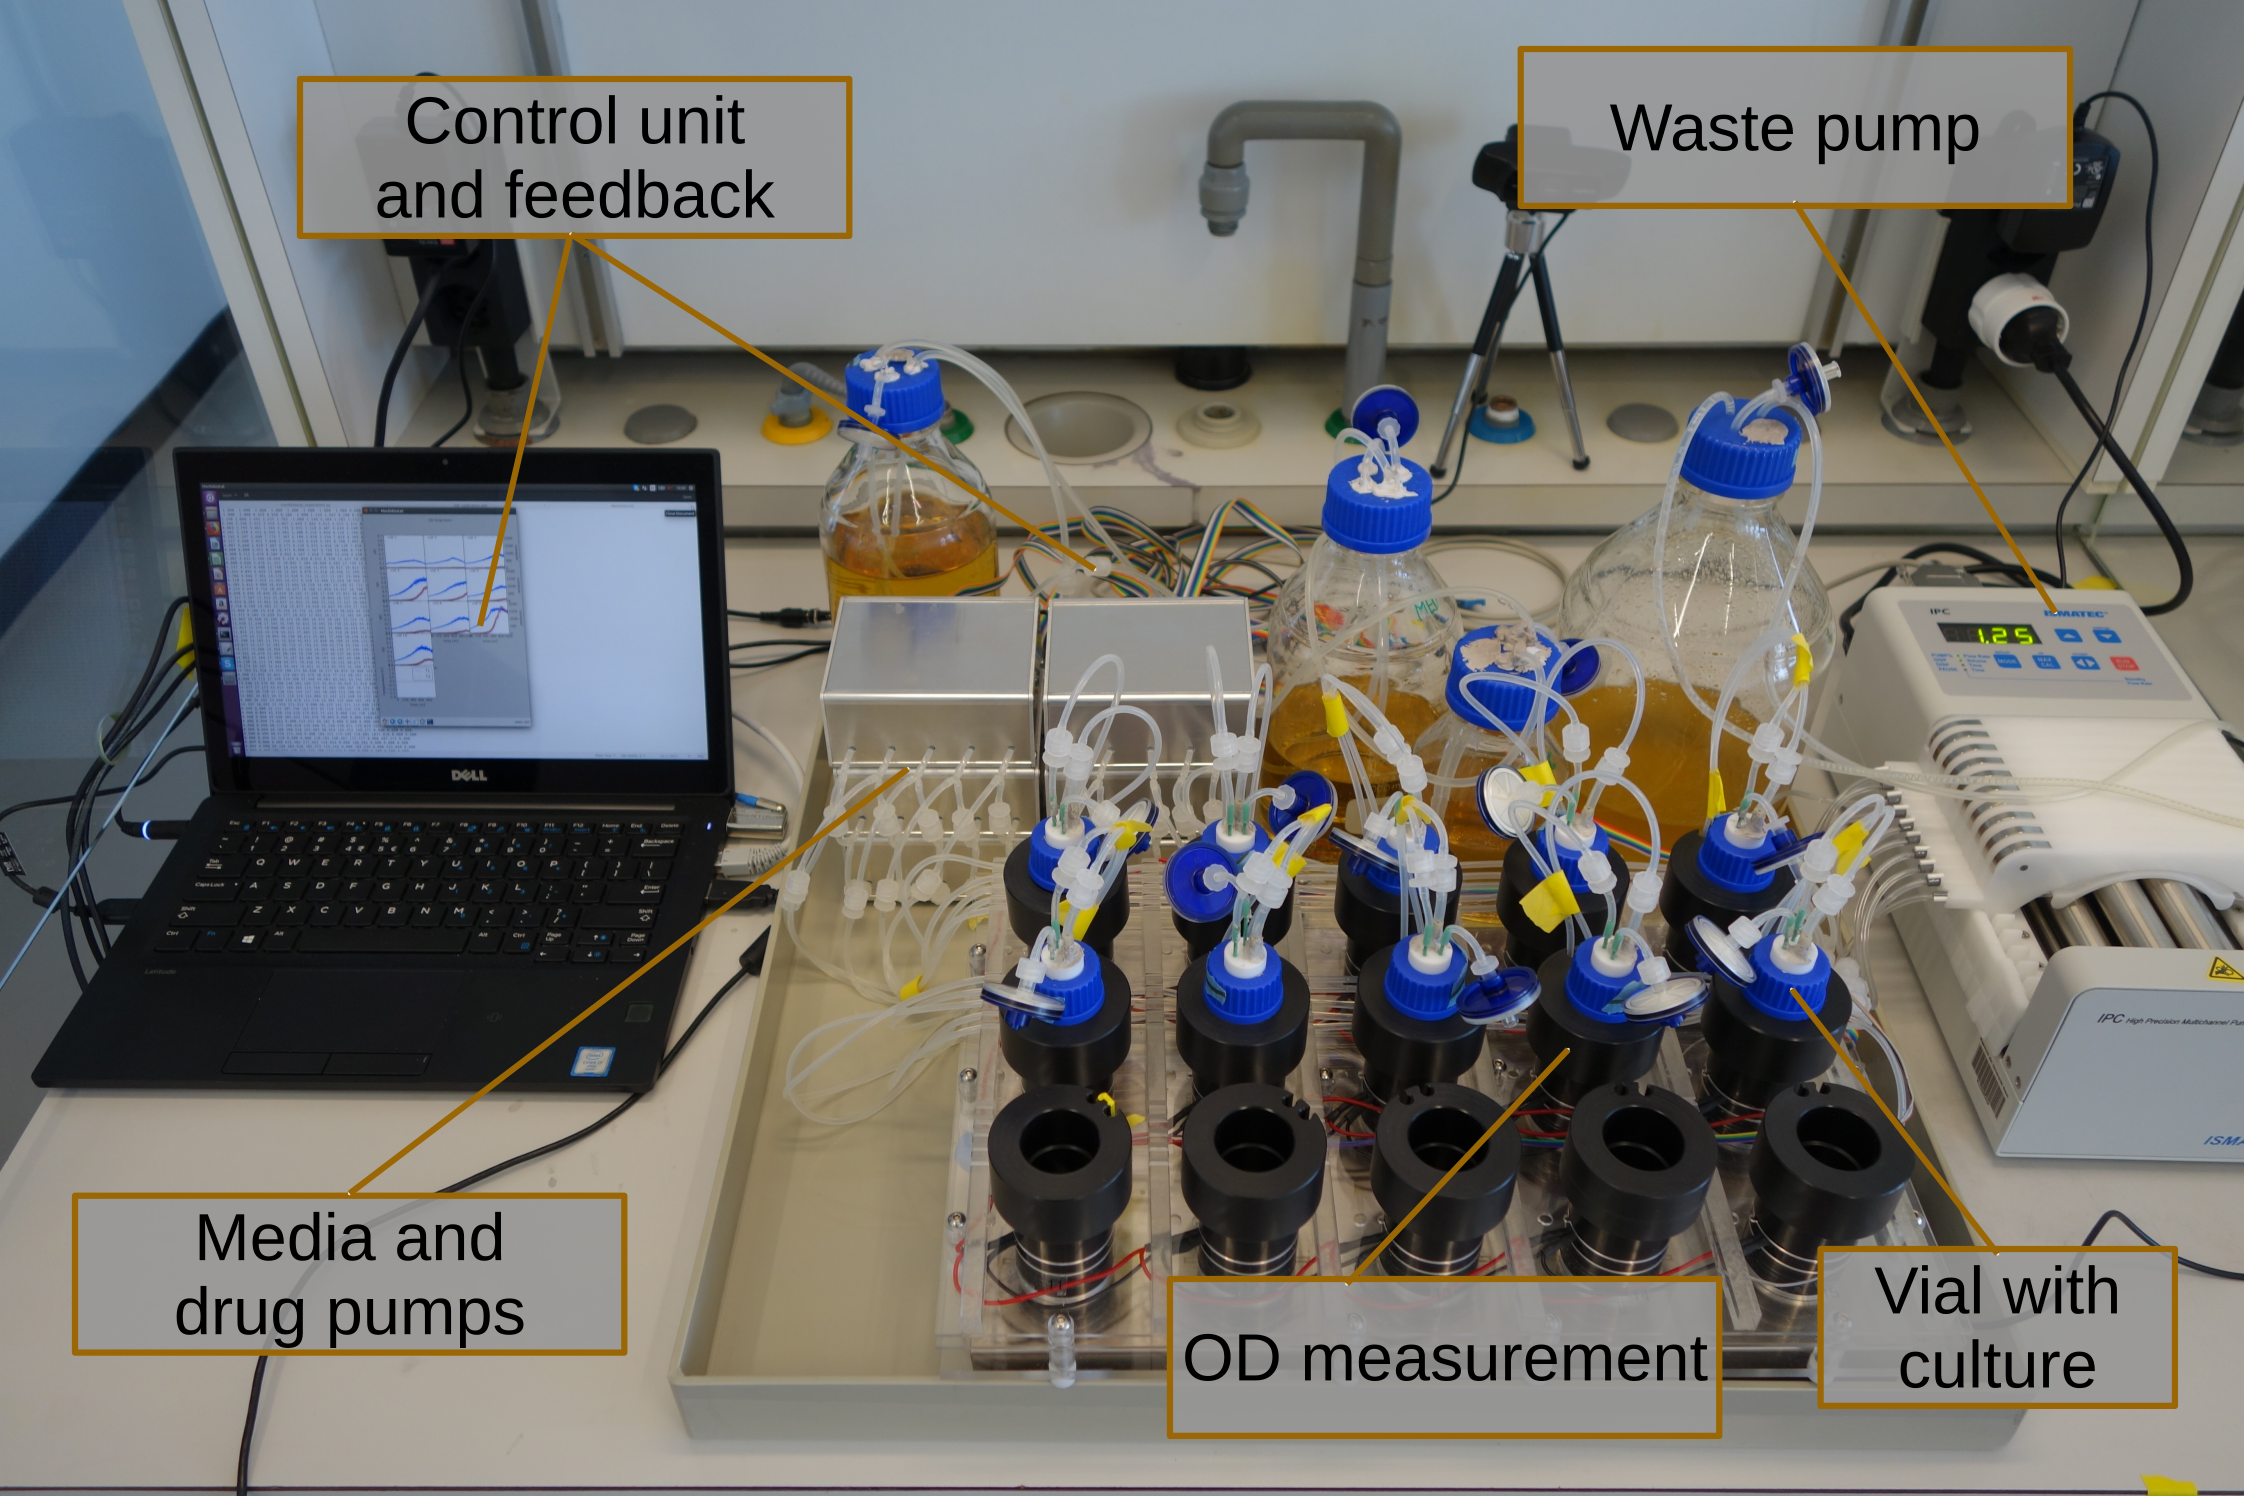
\includegraphics[width=0.7\textwidth]{setup_annotated_inksacpe.png}
	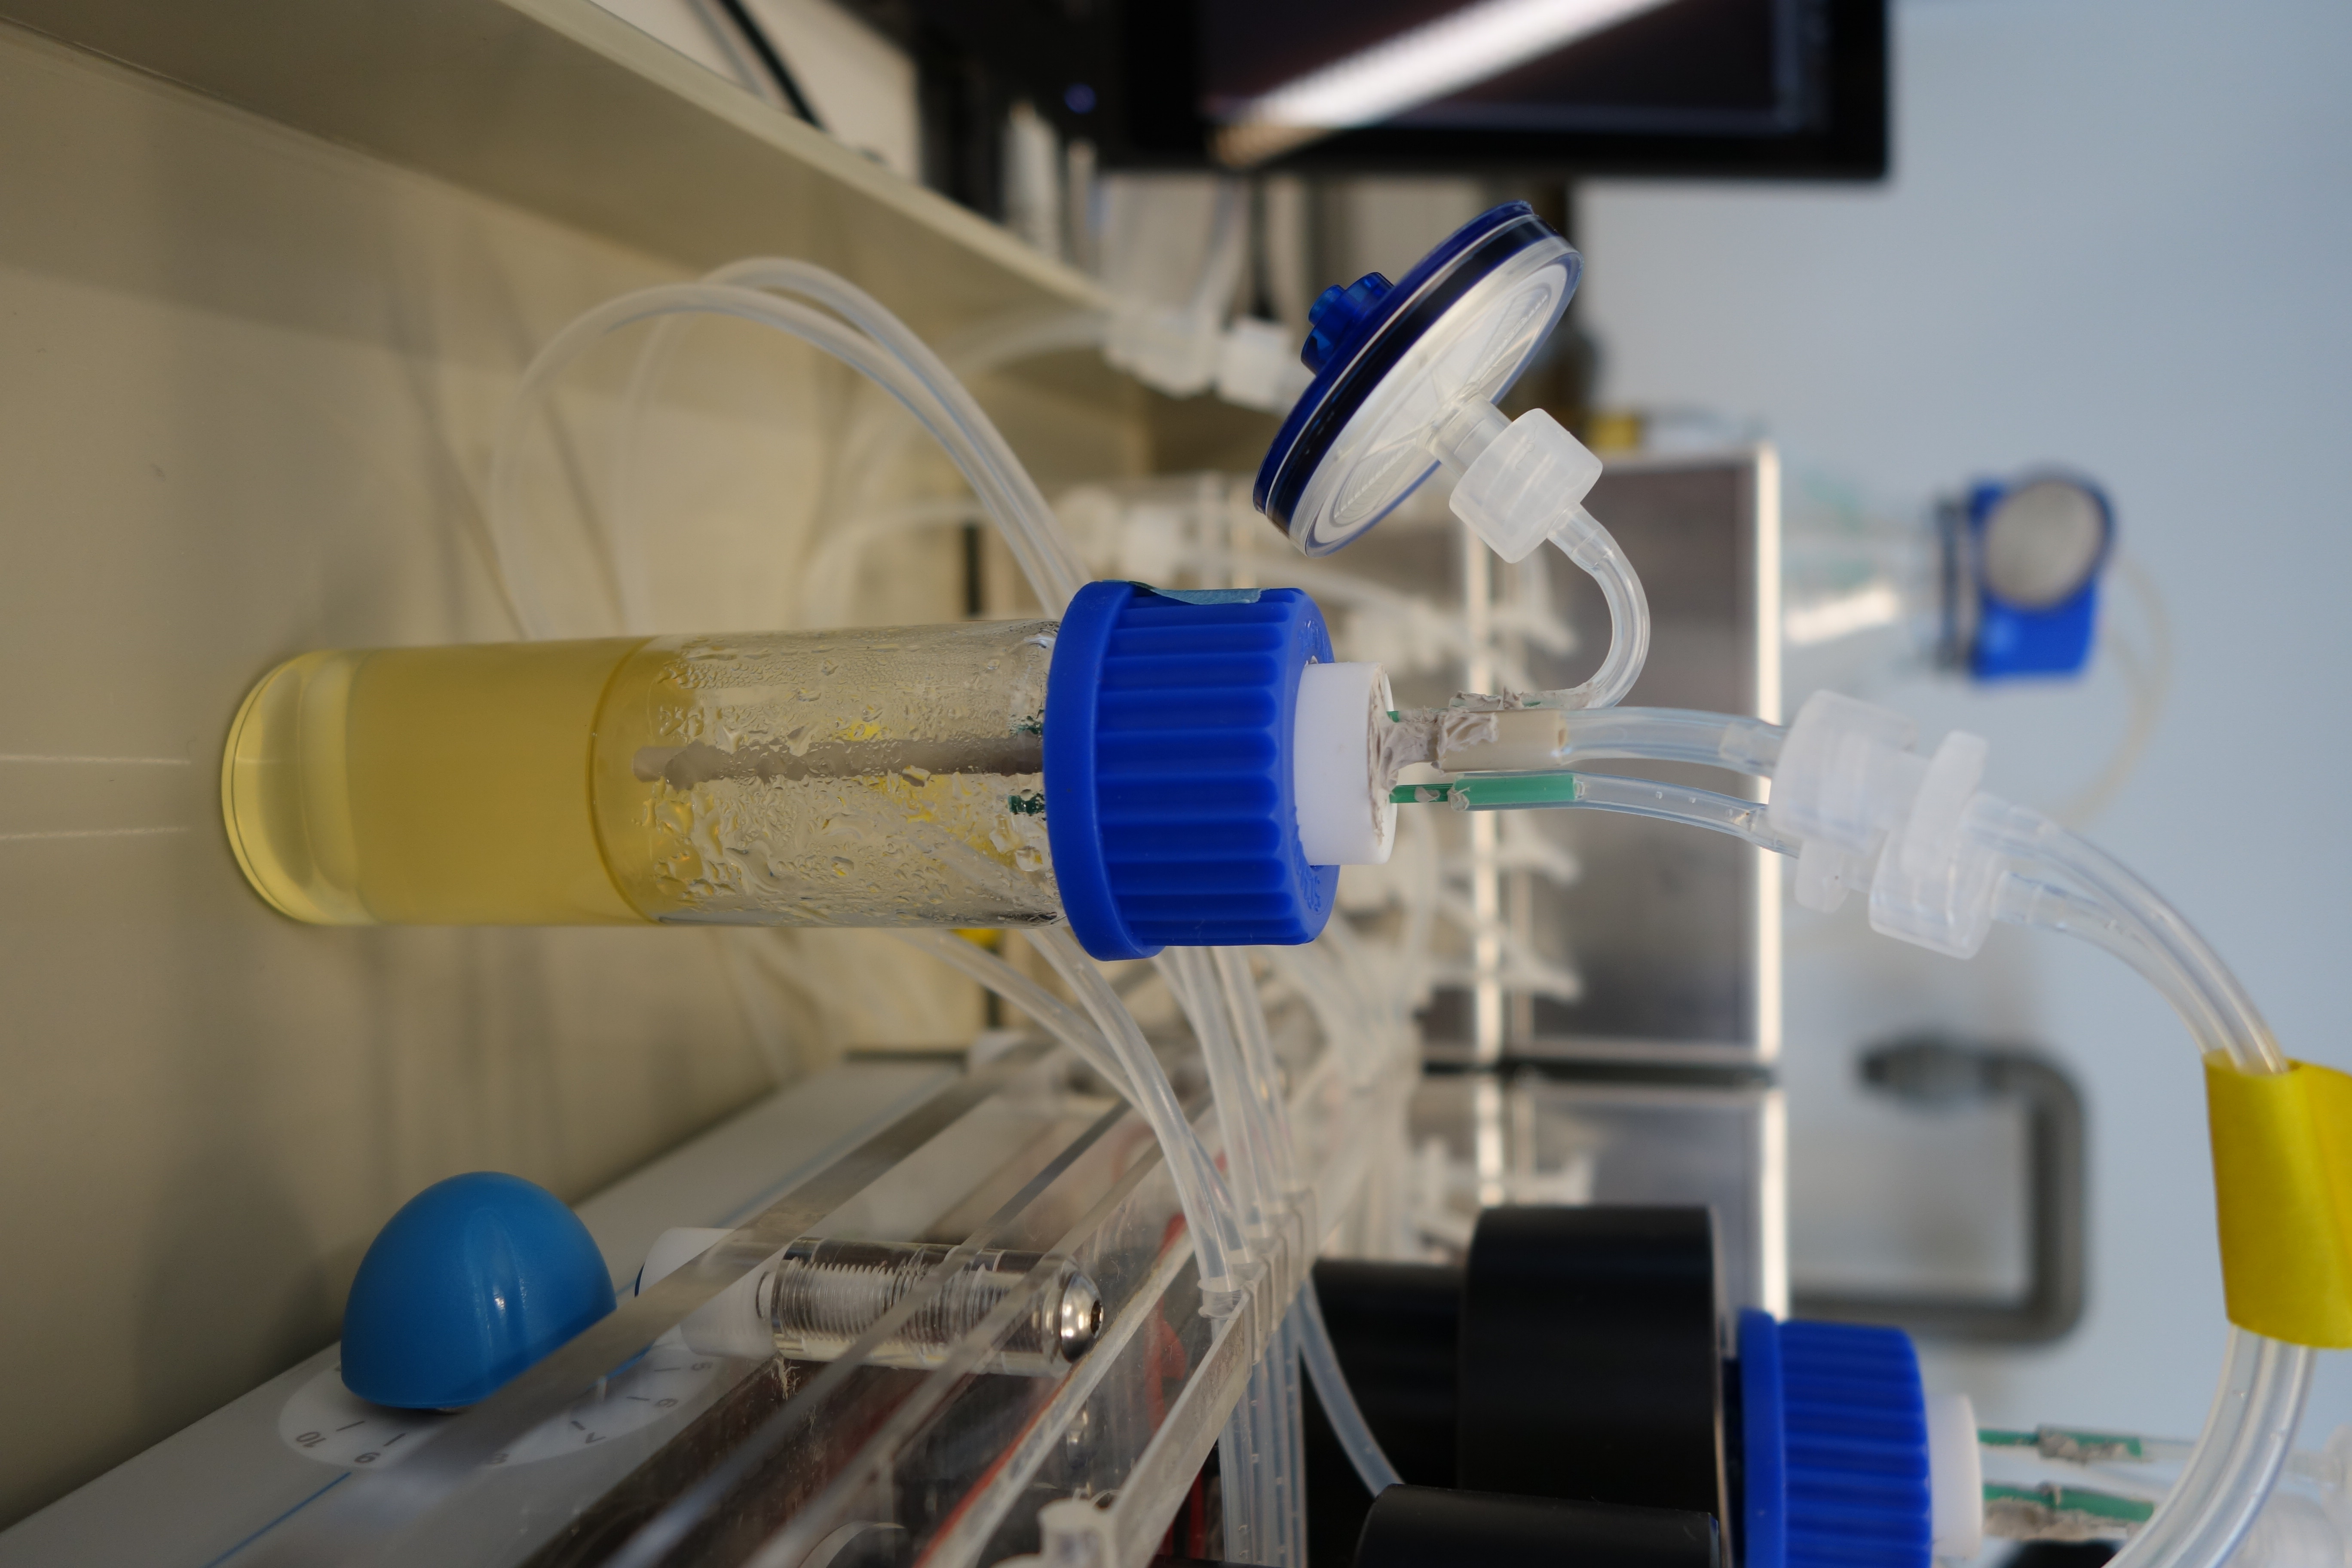
\includegraphics[width=0.4\textwidth,angle=90]{vial.JPG}
	\caption{Left: Overview of the morbidostat setup. The microcontroller is located behind the drug and media pumps. Right: One vial with all the inlets.}
	\label{figure:morbidostat_setup}
\end{figure}  
The left figure \ref{figure:morbidostat_setup} shows the morbidostat setup.
As a base for our built we used a magnetic stirrer with 15 slots. On that stirrer we placed three layers of acrylic glass through which we inserted black plastic rings which acted as our vial holders and optical density (OD) measuring units. 
The vials placed in the vial holders had three inlets as shown in the right Figure \ref{figure:morbidostat_setup}. One inlet was used to inject media or antibiotics, one for removing volume exceeding the culture volume and the last one to mount an air filter for pressure equilibration. \\
For Testing the hardware, we built the morbidostat in the open as shown in the Figure \ref{figure:morbidostat_setup}. For the actual experiments we placed the morbidostat inside a hypoxi-station in a bio safety lab 2. This allowed us to culture the bacteria at 37 \degree C but also to increase the safety. 


\subsection{OD measuring units}
For measuring the ODs we sent a ray of light through the cultures. This ray was scattered by the cells which means that ray was thrown off by the cells in multiple directions. With the help of a phototransistor we could measure the scattering with analolg pins of the microcontroller. Because the scattering was proportional to the cell density, we could translate the scattering into an OD by calibration. \\
One OD measuring unit integrated in the vial holder is shown in  the right Figure \ref{figure:OD_unit}. Every unit consisted of a light emitting diode (LED) and a phototransistor. We chose OPB608A as a LED with a peak wavelength of 890 nm and PT 333-3C as a phototransistor, both from from TT electronics. For each unit the LED and the phototransistor were placed in a 135 \degree \space angle inside the vial holder. Both components were in direct contact with the glass vial.
The 15 OD measuring units were divided into three groups of five units which corresponds to one row of vials of the morbiostat. For every group the LEDs and phototransistors were both connected to independent 5 V circuits. The circuits of one group are illustrated in the left Figure \ref{figure:OD_cirguit}, where the LED circuit is shown orange and the photoransistor cicruict in blue. \\
The LEDs were constantly on sending rays of light through the cultures. When an OD measurement was initiallized the scattering was detected with the phototransistors. Light reaching the phototransistor caused an opening in the semiconductor from the phototransistor which led to an amplification of the current. This current reached a potentiometer connected in serial over which we measured the voltage with an analog pin of the microcontroller. The opening of the semiconductor altering the measured voltage correlated with how much light reached it. More cells caused more scattering and more light reaching the semiconductor. Therefore, there was a linear correlation between the measured voltage and the cell density in the suspension. \\

\label{section:OD}
\begin{figure}
	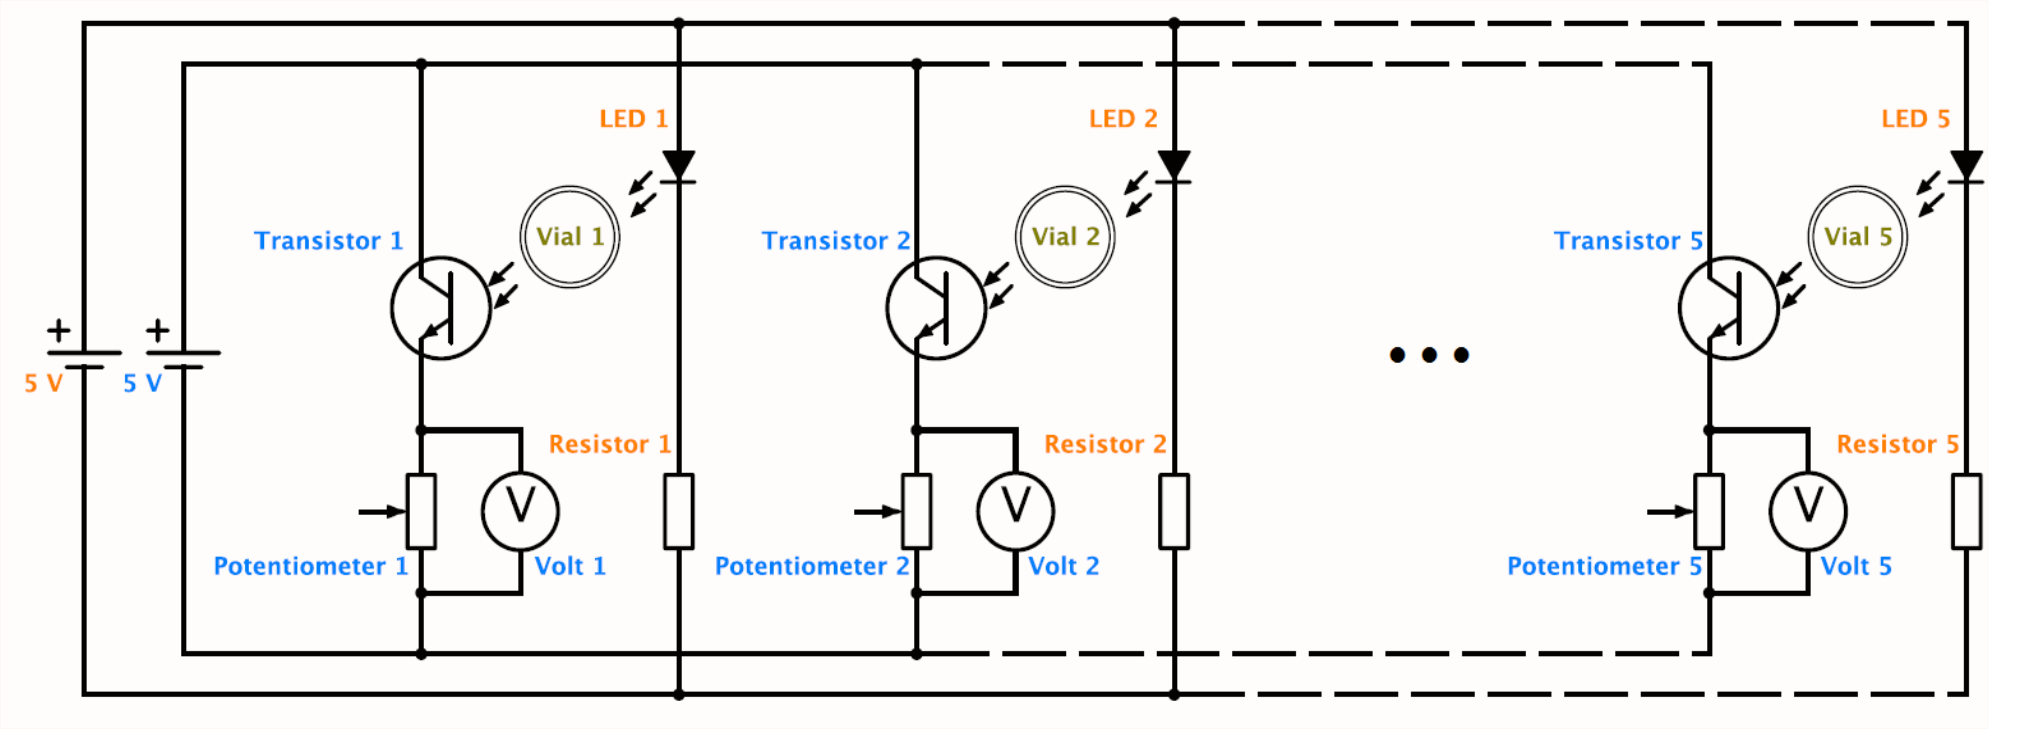
\includegraphics[width=0.6\textwidth]{OD_setup.png}
	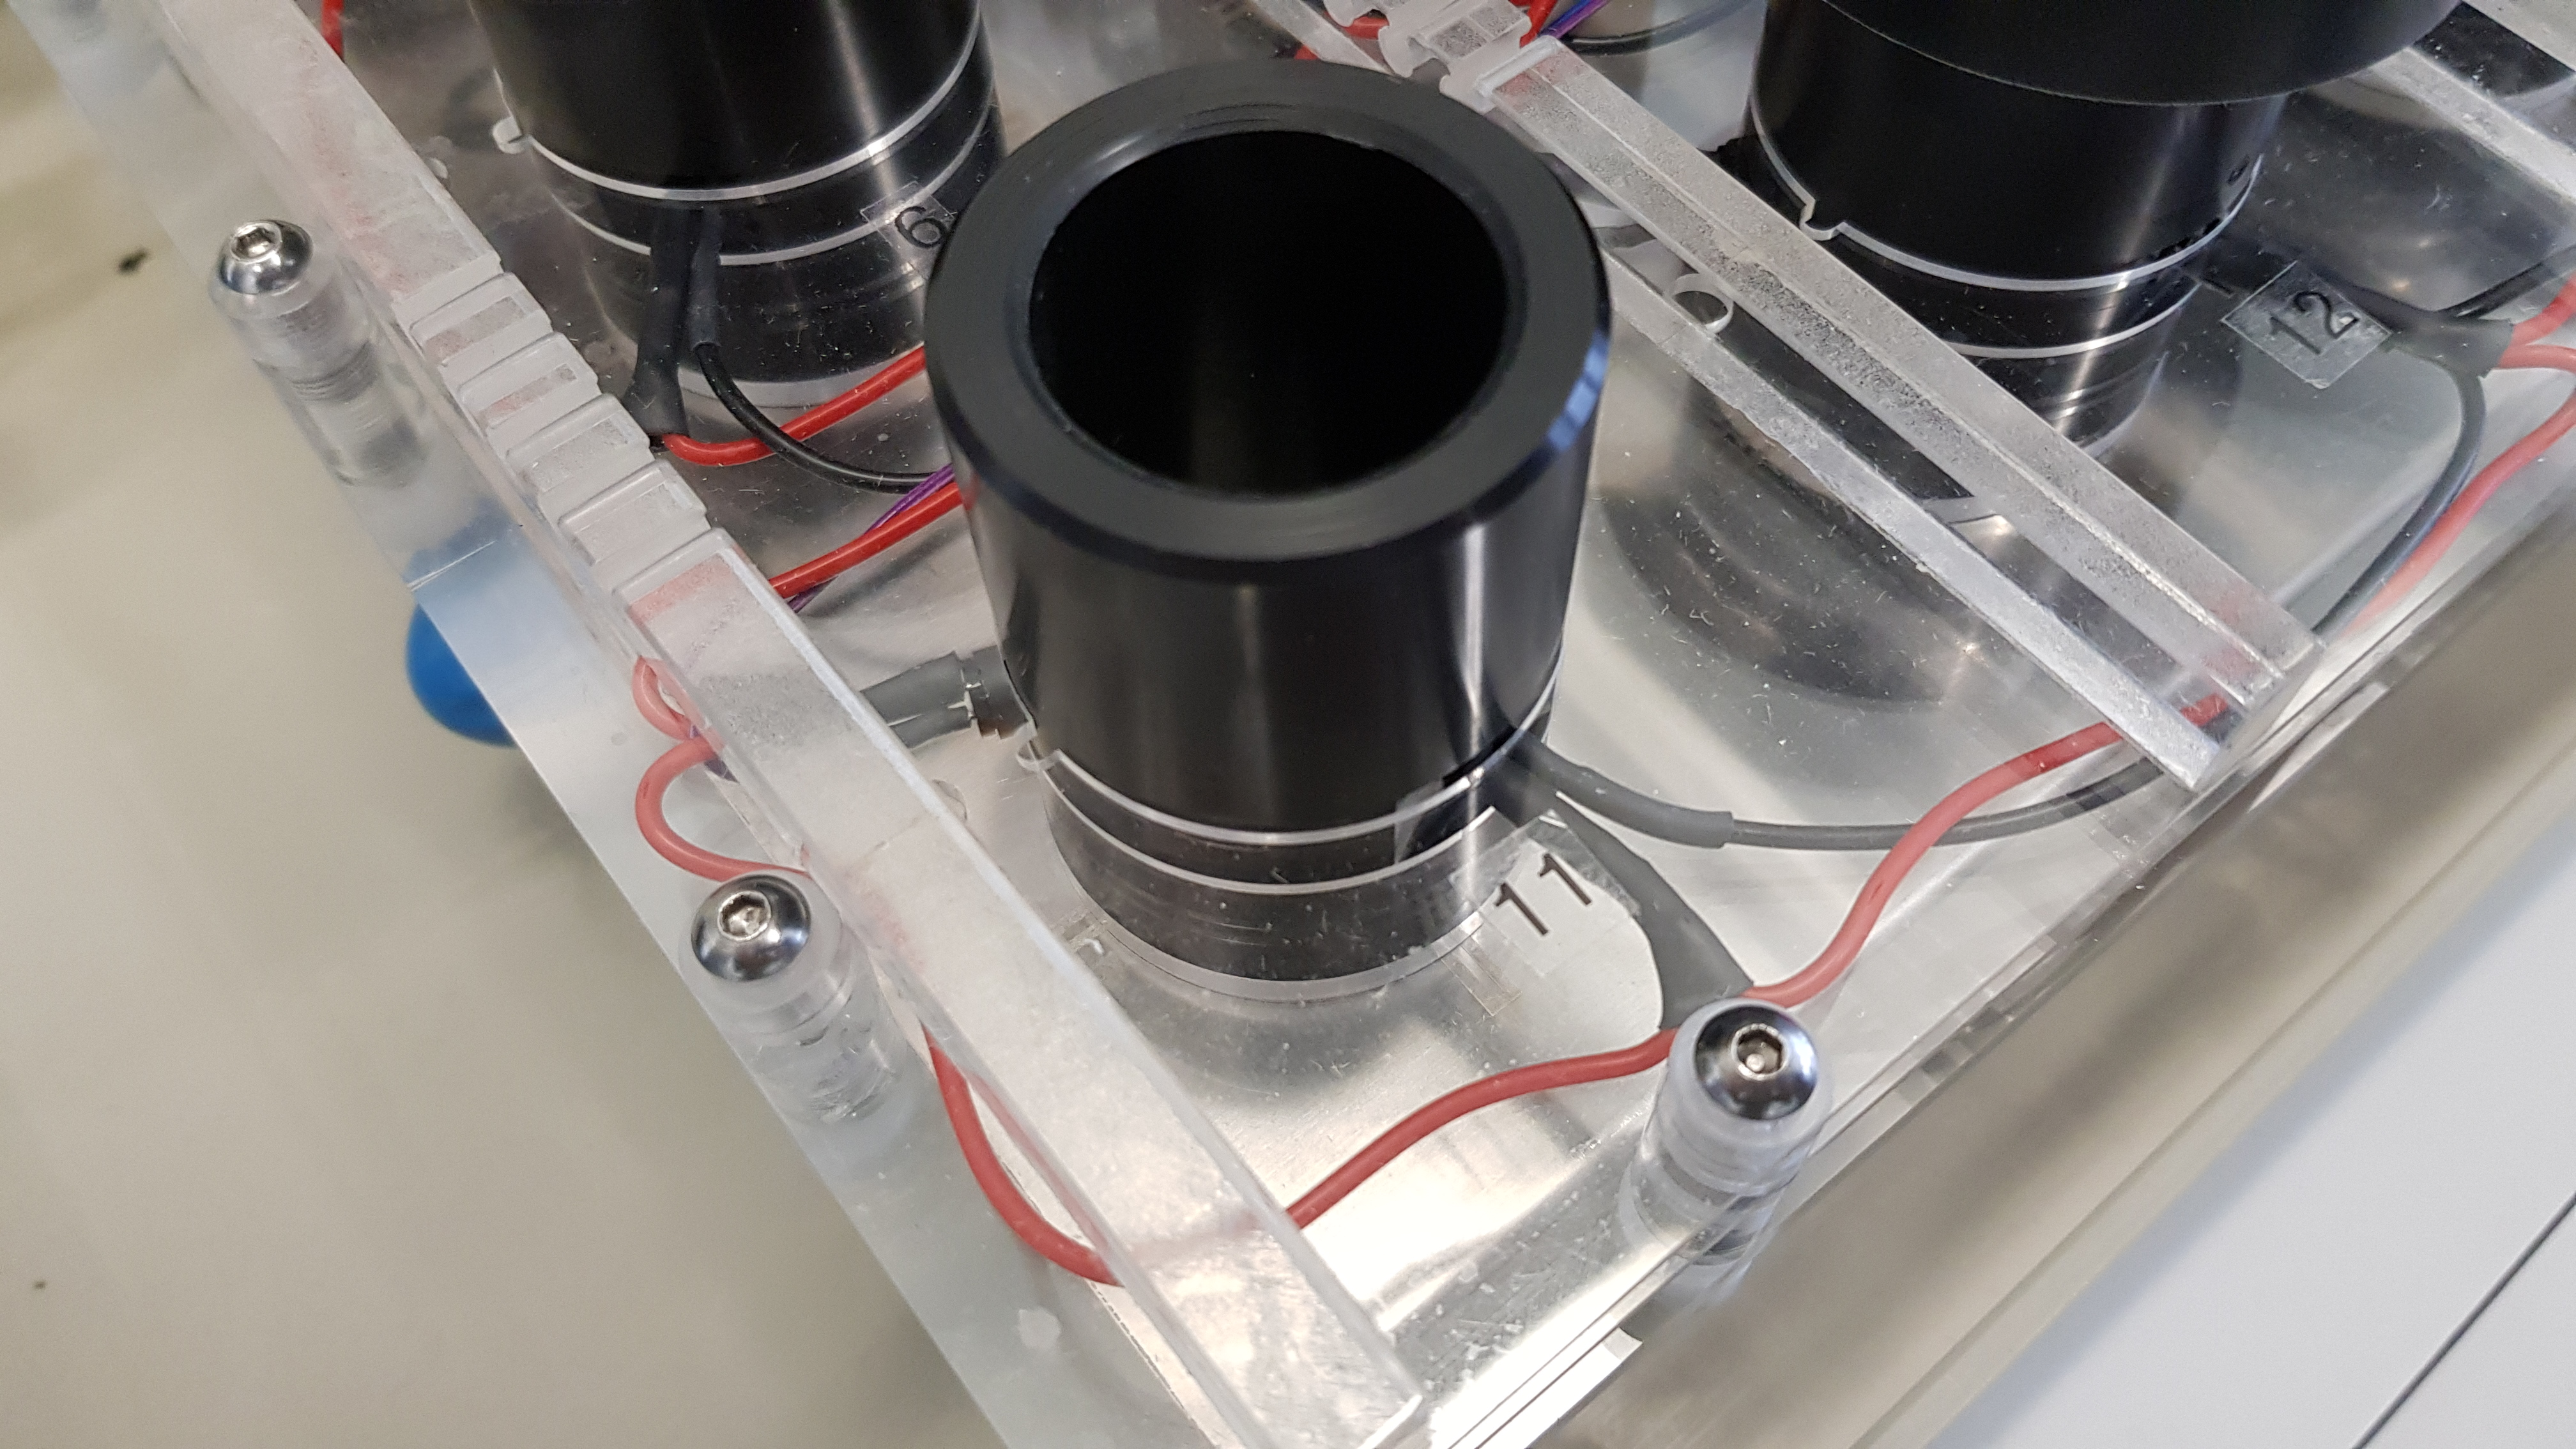
\includegraphics[width=0.3\textwidth]{OD_unit.png}
	\caption{Left: Circuit for parallel connected LEDs (orange). Each LED is connected in serial with a x \textOmega \space resistor. The circuit of the phototransistors is shown in blue. The phtototransistors are connceted in parallel. Each phototransistor is connected to a potentiometer in serial over which the voltage is measured with an analog pin of the microcontroller.}
	\label{figure:OD_cirguit}
	\label{figure:OD_unit}
\end{figure}

\subsection{Pumps and tubing} 
\begin{figure}
	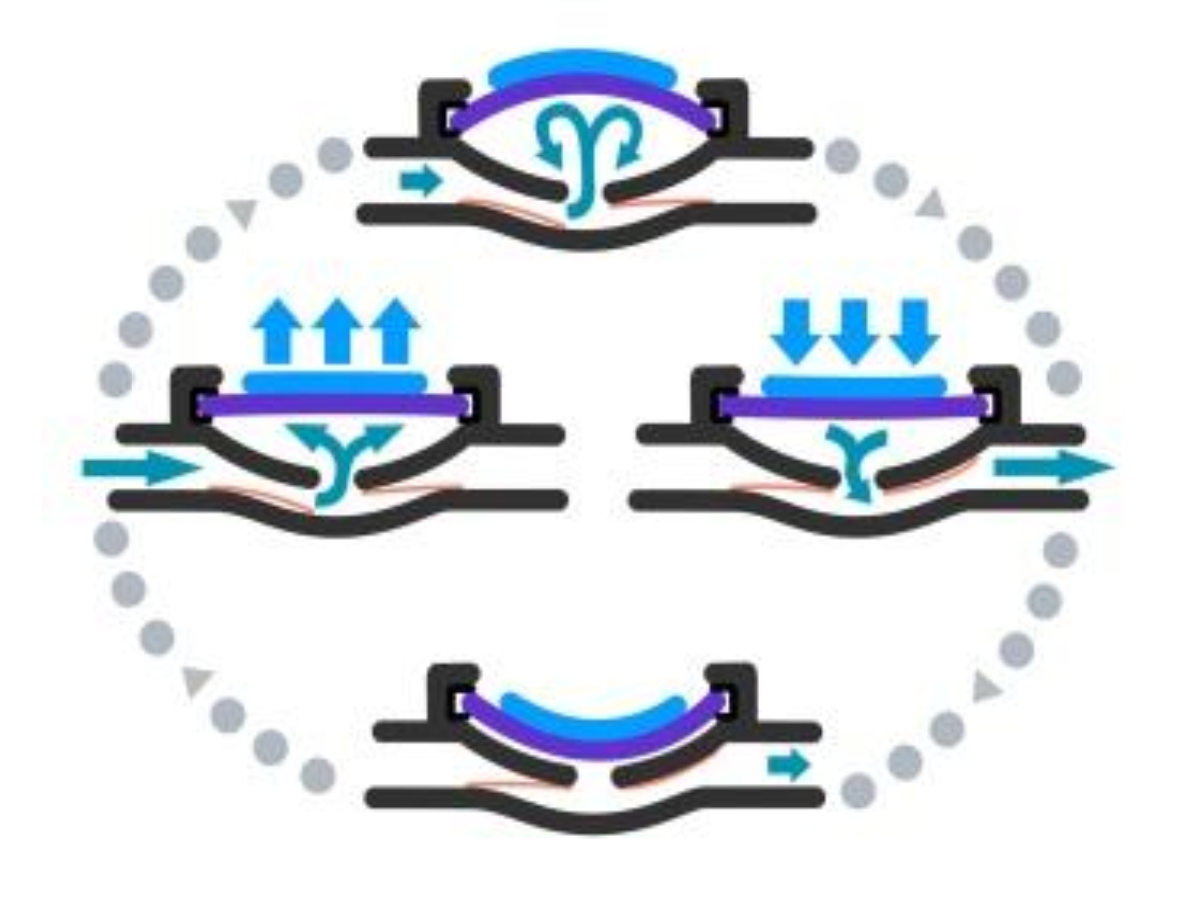
\includegraphics[width=0.2\textwidth]{piezo.png}
	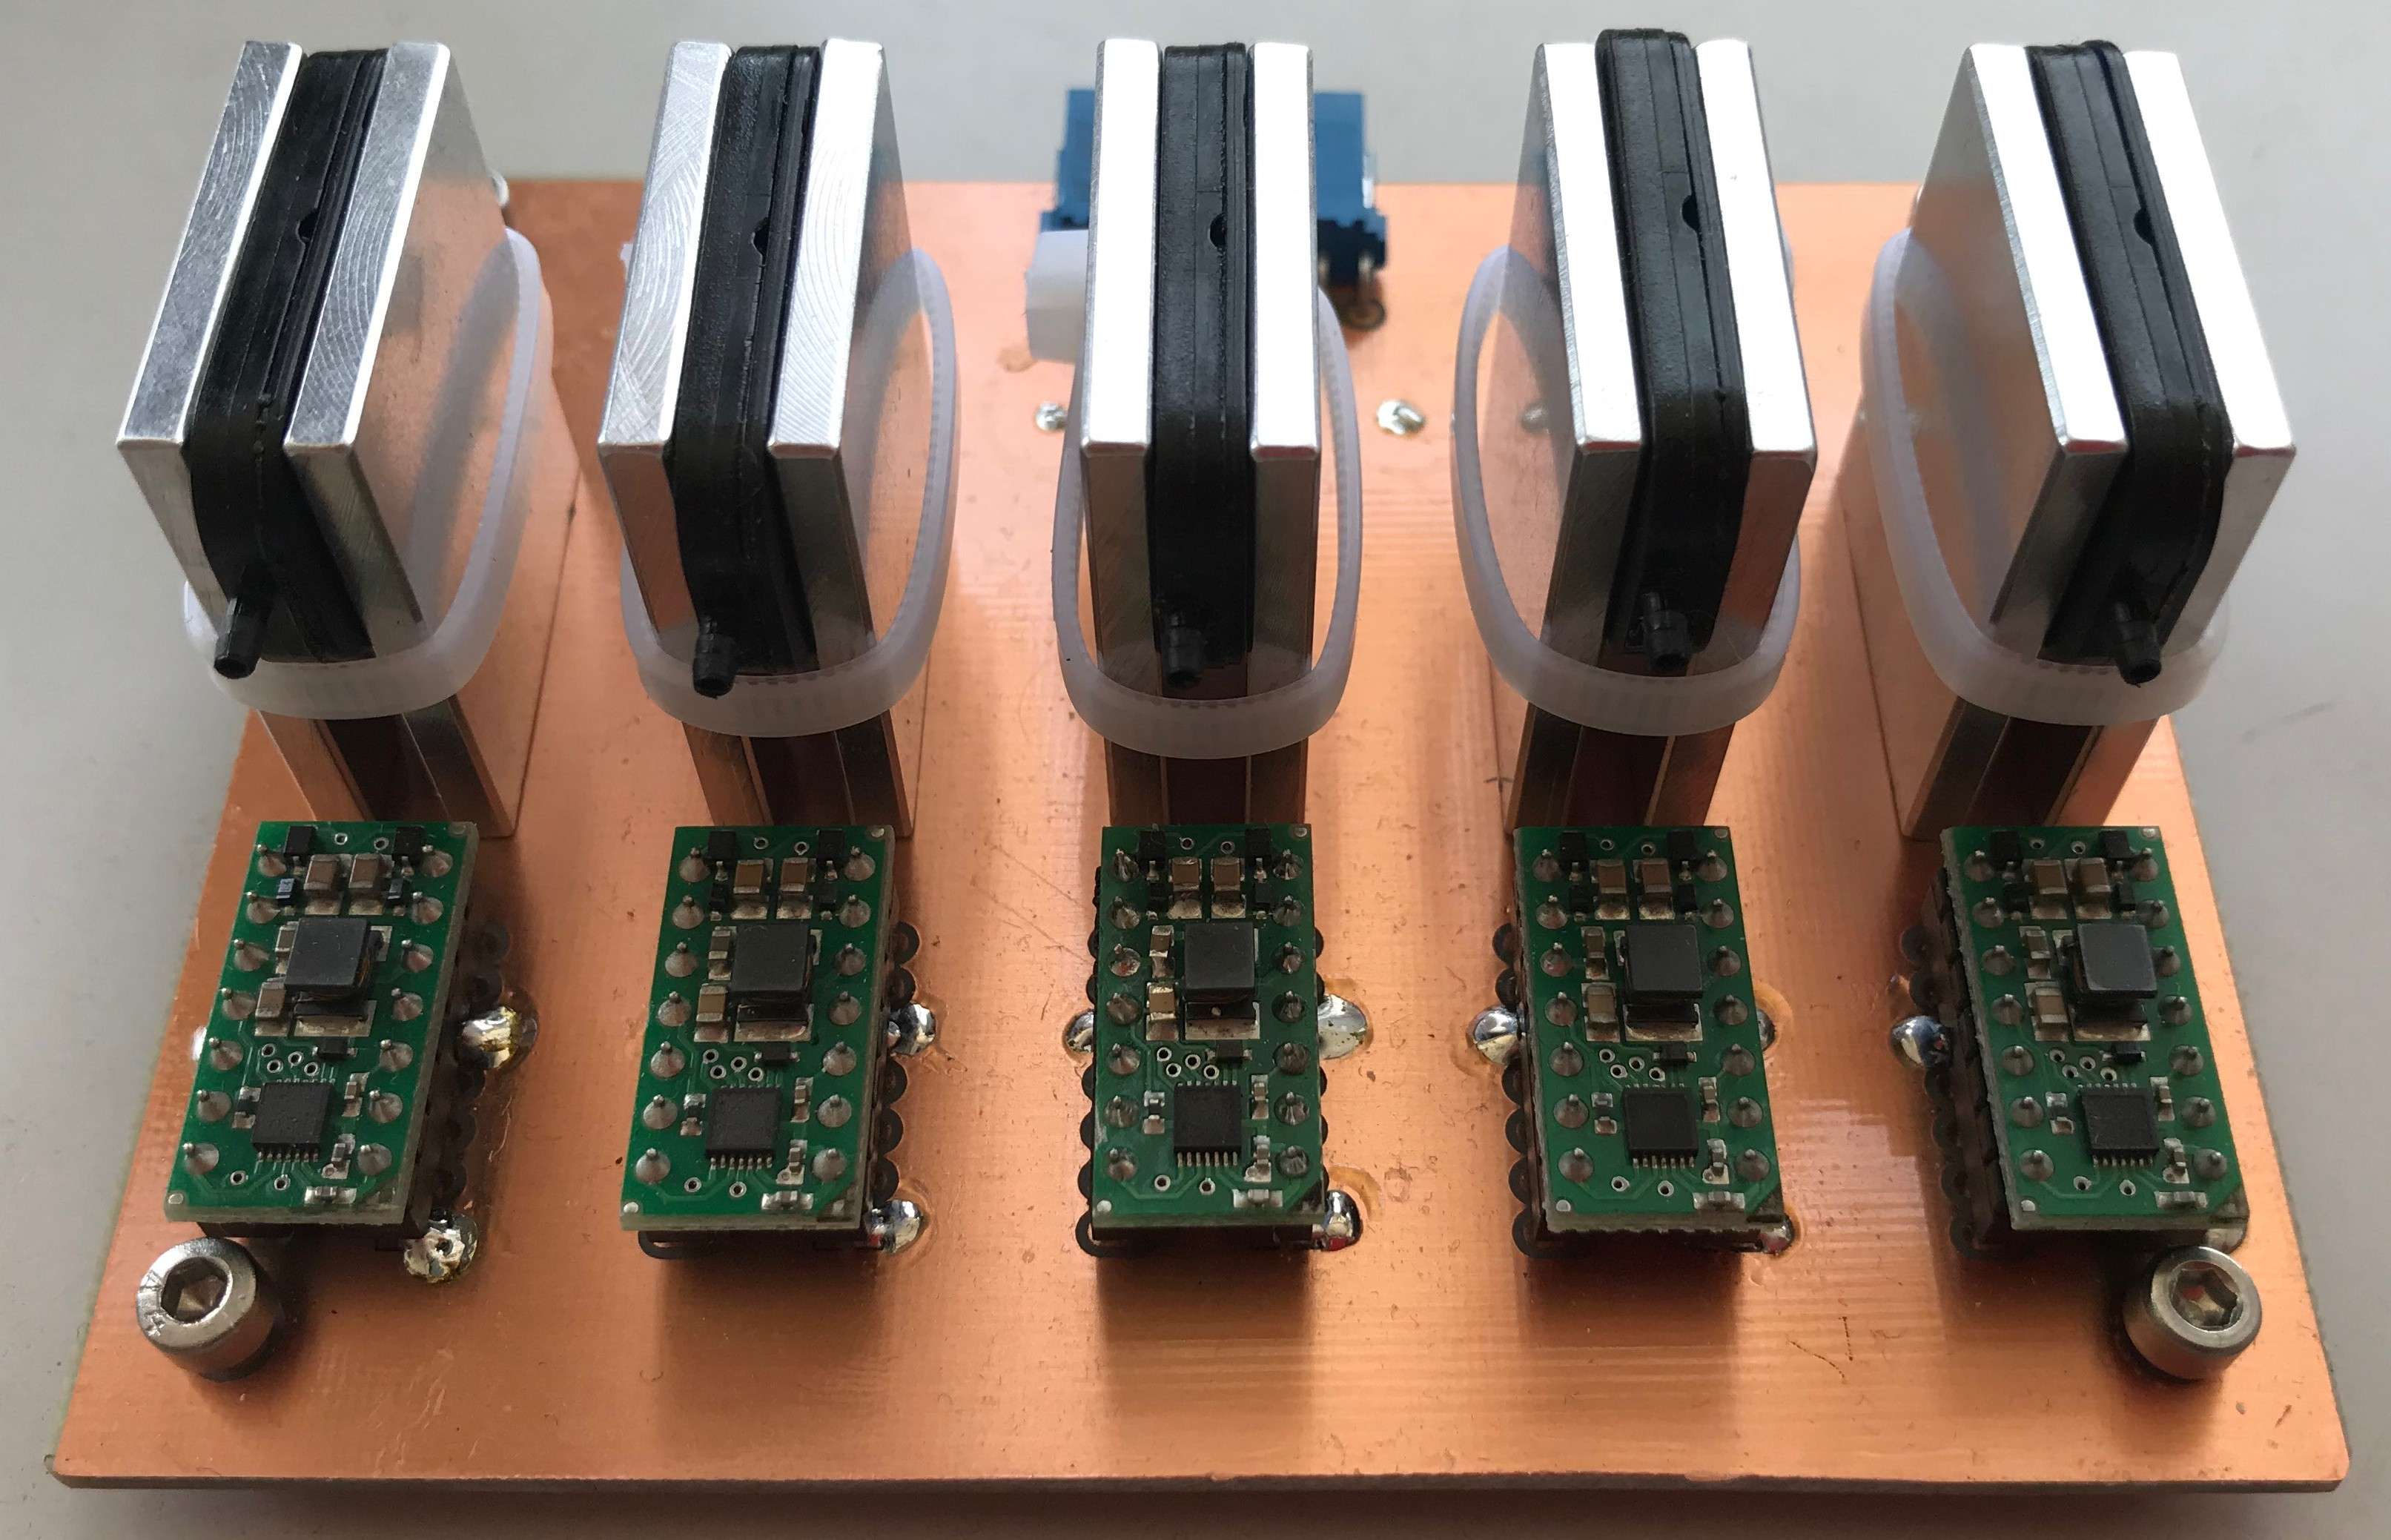
\includegraphics[width=0.4\textwidth]{board.JPG}
	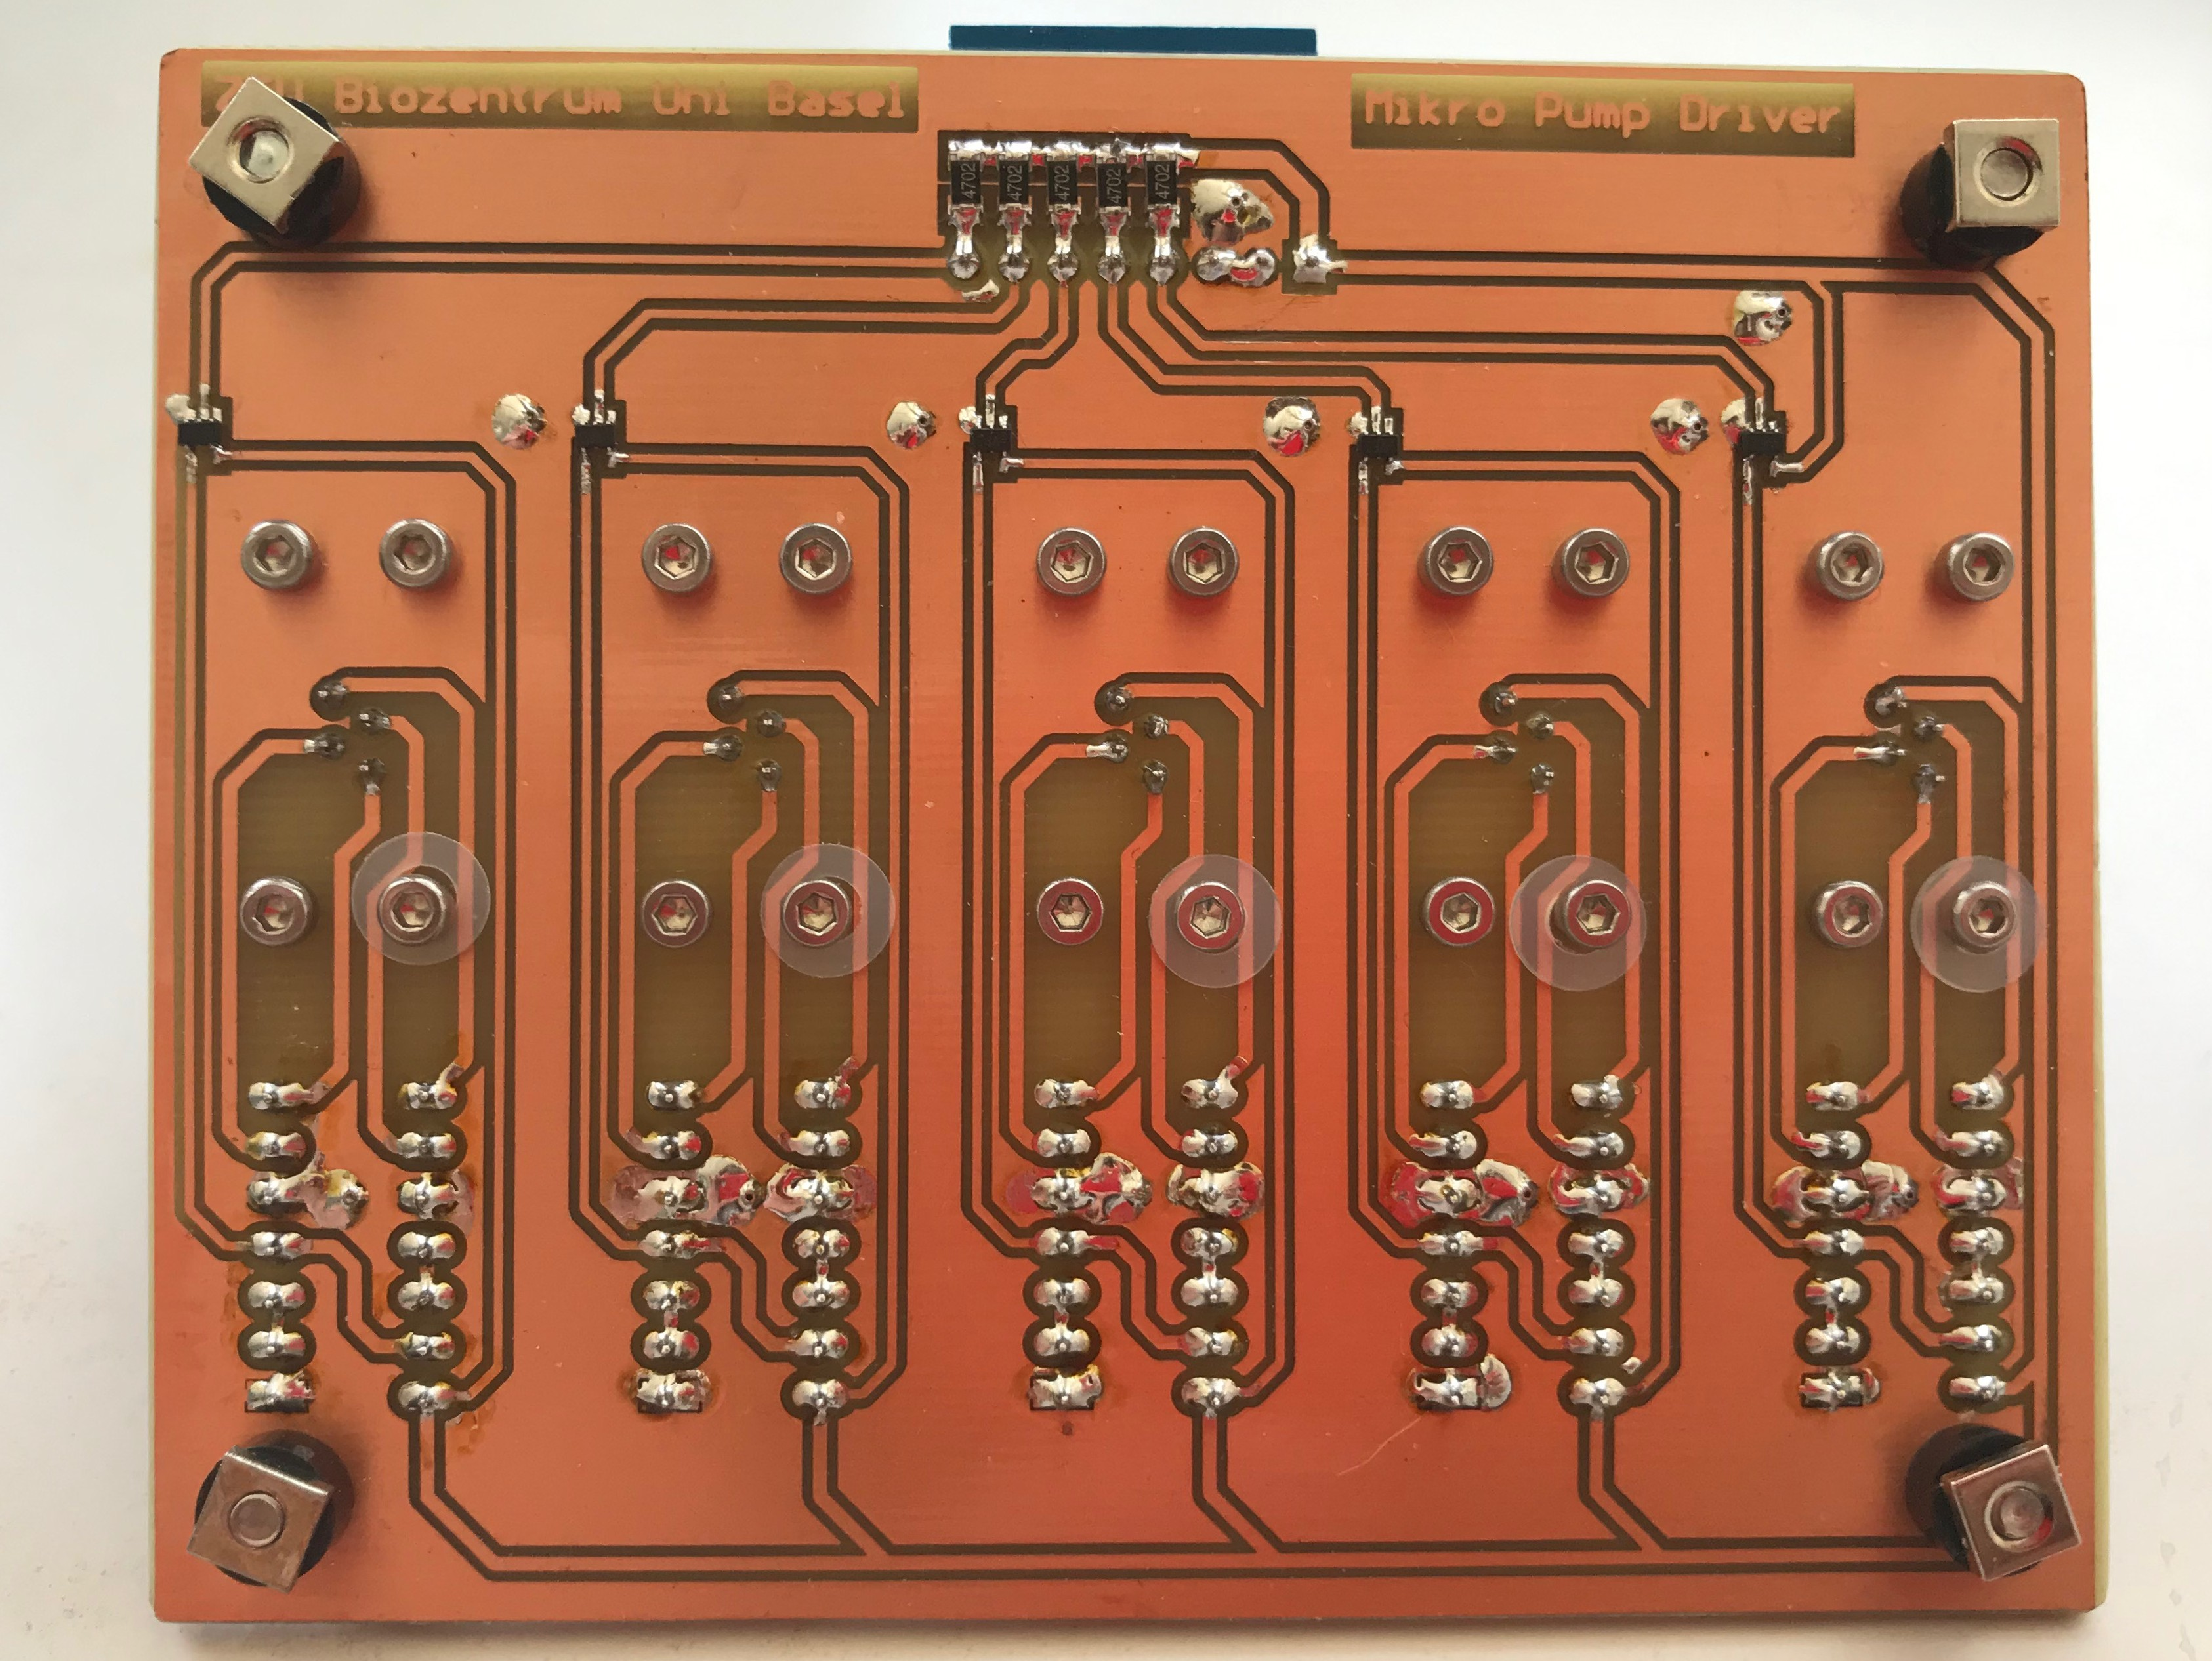
\includegraphics[width=0.4\textwidth]{board_below.png}
	\caption{Left: Principle of the piezo pumps. Top state: Piezo ceramic (purple) mounted on a membrane (blue) is relaxed.Left valve is open (orange), right valve  is closed, liquid enters. Right and bottom state: Voltage is applied to the piezo ceramic deforming the membrane resulting in a down stroke. Left valve is closed, right valve is open Liquid exits to the right. Voltage decreases again and the piezo ceramic enters its relaxed state again \cite{piezo_pumps}}. Middle: Top view of a circuit board with five pumps and five controllers. Right: Bottom view of a circuit board. 
	\label{figure:pumps}
\end{figure}
\begin{figure}
	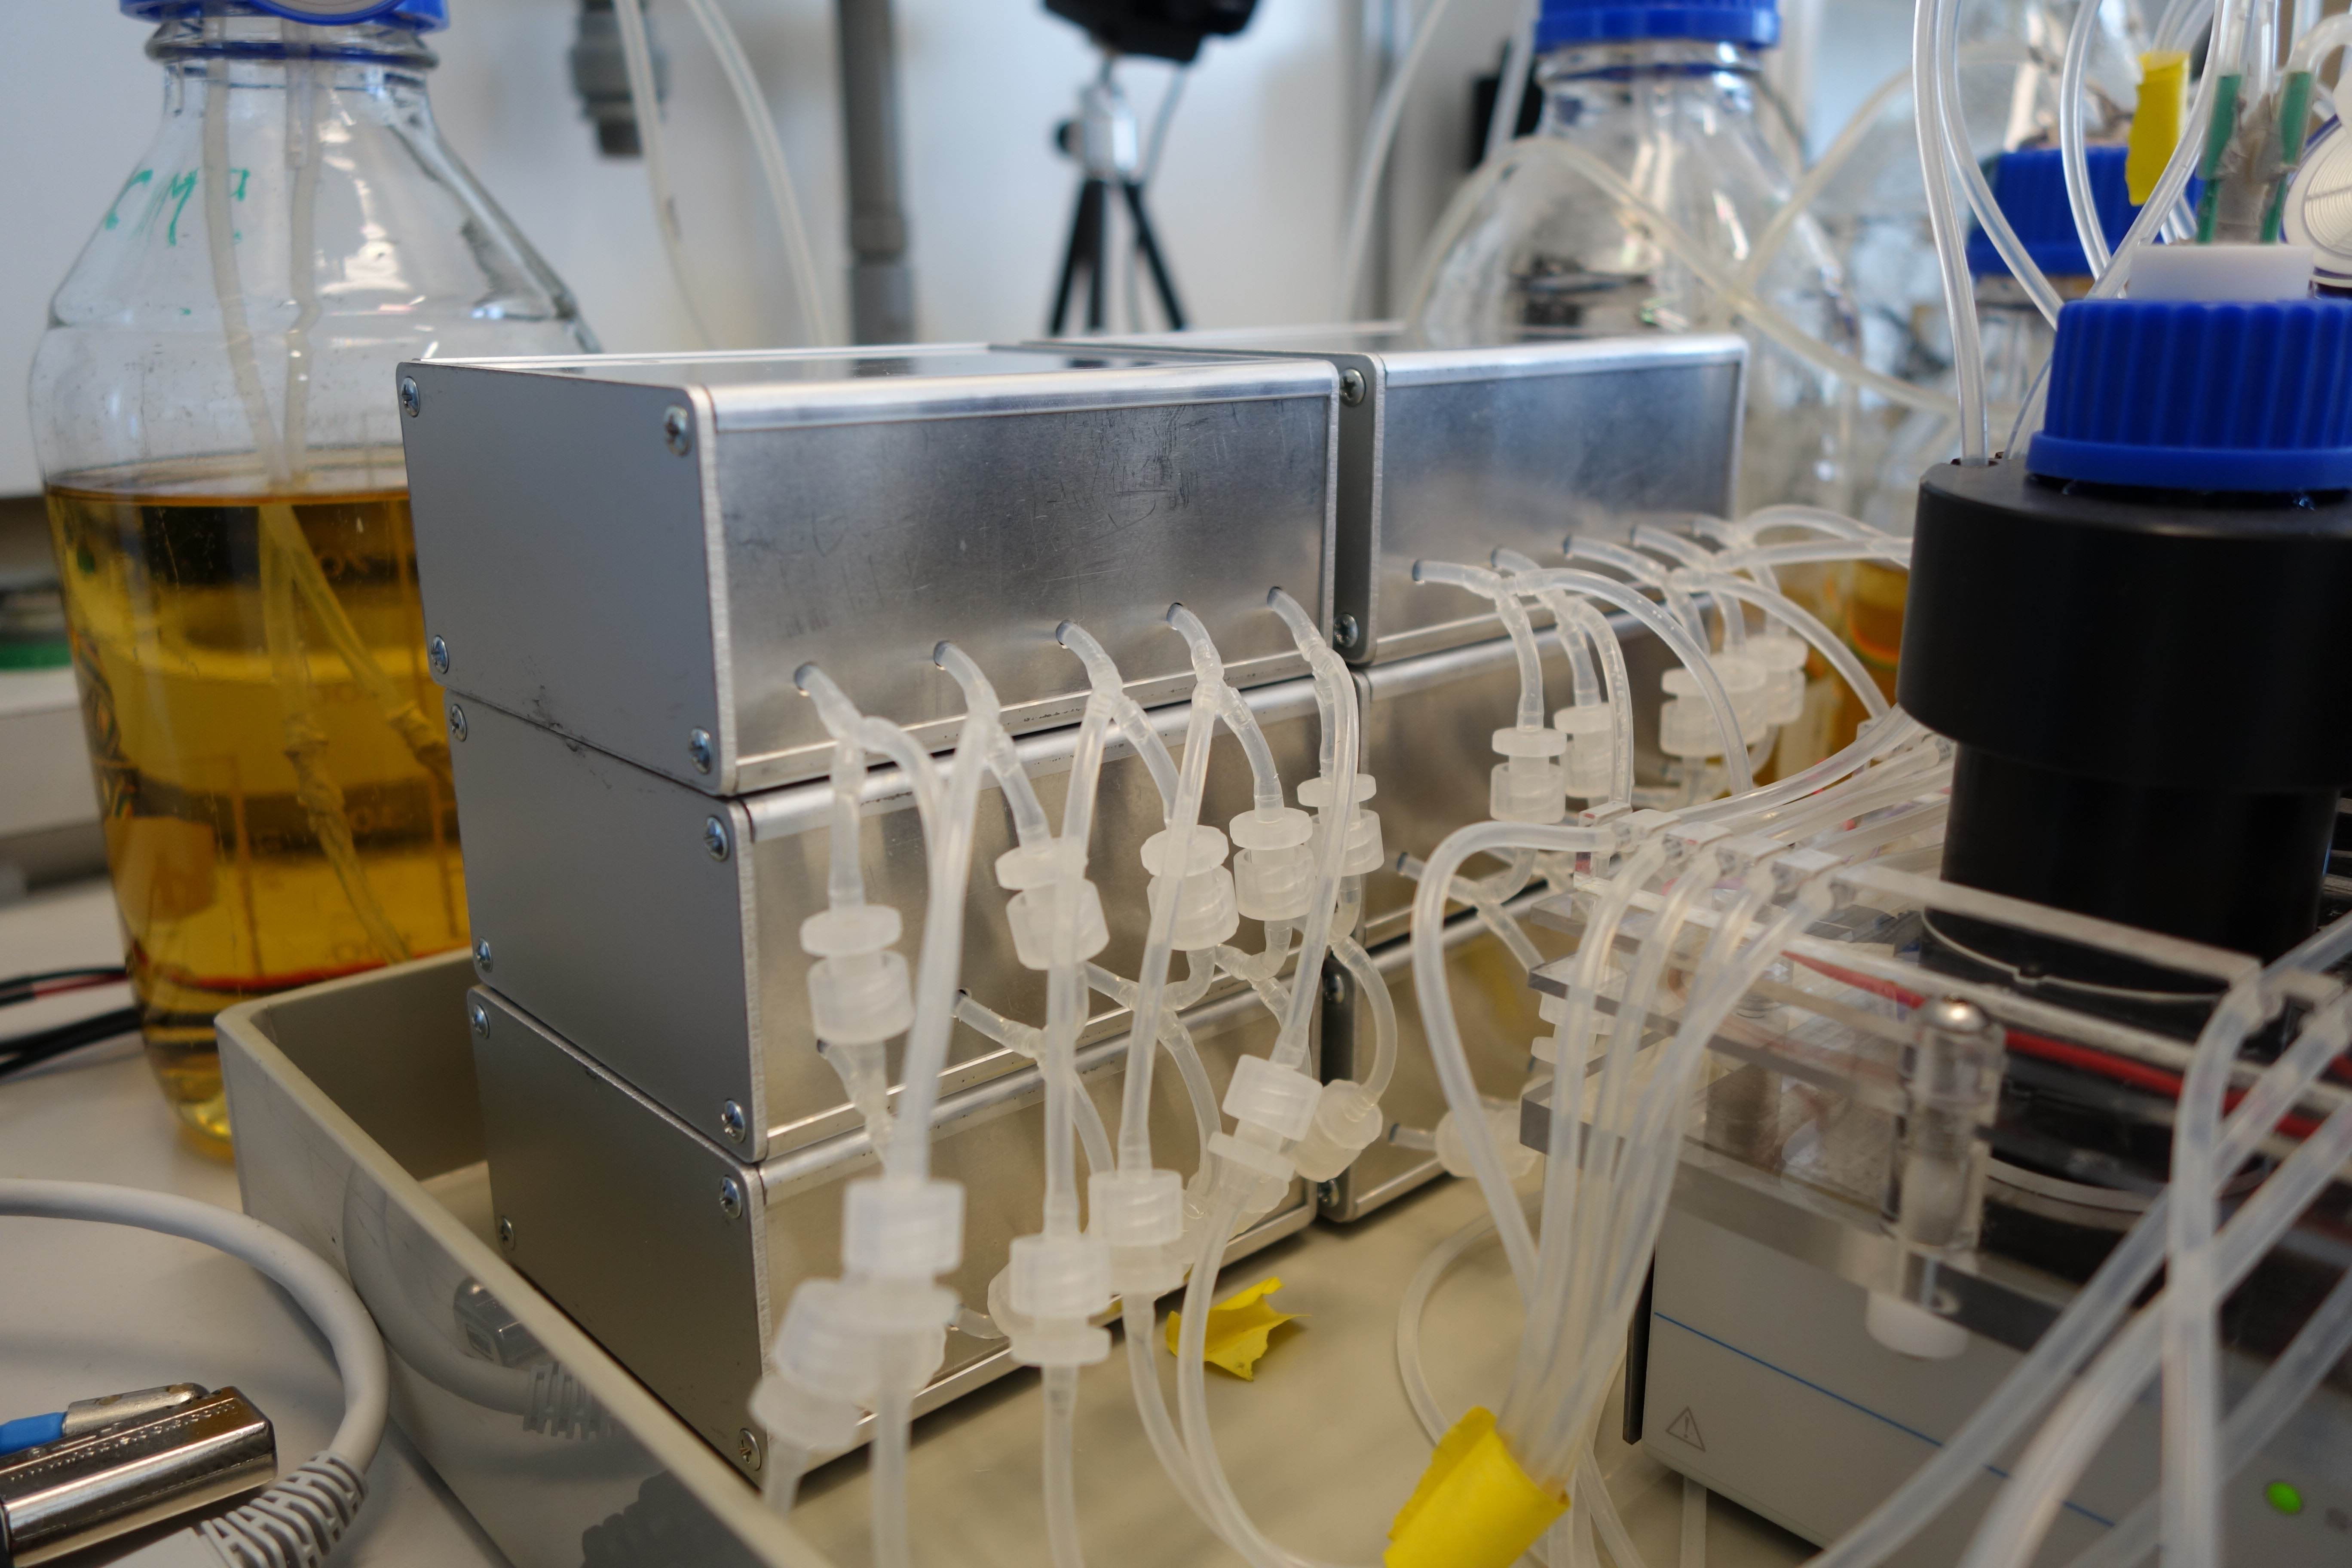
\includegraphics[width=0.5\textwidth]{pump_blocks.JPG}
	\caption{Figure left: Vial setup. Figure right: One row of five pumps represents one row of five vials. Since every vial is connected to three pumps, three rows of pumps are stacked on top of each other and connected column by column. This means that one column of three pumps is responsible for injection fluid into one vial. Every outlet from a pump from one column is connected, in order that there is just one tube going to one vial. }
	\label{figure:tubing_setup}
\end{figure}
Every vial was connected to three injecting pumps. One pump was responsible for injecting media, one for injection a low-concentrated antibiotic and one for injecting a high-concentrated antibiotic. Mixing of desired antibiotic concentration was possible by controlling the run times of the pumps.
We chose mp6 pumps from microComponents because of their very compact build. The functional principle of the pumps is shown in the left Figure \ref{figure:pumps}. We achieved a steady flow rate of the pumps with the mp6-OEM controller from microComponents. On one circuit board five pumps with five mp6-OEM controllers were mounted which is shown in the middle Figure \ref{figure:pumps}. Each mp6-OEM controller was connected to one pump, a 5 V power supply, a ground and a digital pin of  the microcontroller which allowed computer controlling the run times of every pump. The circuit boards were mounted in a metal box and three of those boxes stacked on top of each other which is shown in Figure \ref{figure:tubing_setup}. By packing five pumps in a box and stacking three boxes on top of each other we were able to connect one row of vials to the whole range of antibiotic concentrations with one stack. Pumps of the lowest box were connected to media, pumps of the middle box to a low-concentrated antibiotic and the pumps of the top box to a high-concentrated antibiotic. We connected the outgoing tubes of the pumps from one stack column by column resulting in one outgoing tube per column as shown in Figure \ref{fiuger:tubing_setup}. Those tubes were led to the vials. This way we connected one vial with three pumps ranging all concentrations and leading just one tube to the vial.\\
Every vial was also connected to a 16-channel peristaltic pump which removed volume exceeding the culture volume through the grey tube show in the right Figure \ref{figure:morbidostat_setup}. 

\subsubsection{Computer controlling the pumps}
In order to control the run times of the pumps a pin of every mp6-OEM controller was conncected with a digital pin of the microcontroller. If the pin of the mp6-OEM controller received a voltage of 5 V the pumps were off, if the pin was set to ground the pumps were on. \\
When we set the digital pins of the microcontroller to ground there was still a low current flowing, resulting in a small voltage. The mp6-OEM controllers reacted very sensitive to this small voltage leading to weird behavior of the pumps. We solved this by inserting a pull-down resistor between the digital pins of the microcontroller and the ground which is shown in the right Figure \ref{figure:pumps}. Additionally an inverter was connected in serial to the digital pins. To turn on a pump the digital pins of the microcontroller was set to 5 V. The inverter connected in serial caused that the pin of the mp6-OEM controller was set to ground and the pumps were turned on. Run time control was possible by setting the digital pins to 5 V for the desired runtime.
The 16-channel peristaltic pumps was also computer controllable because the pumps was also connected to a digital pin of the microcontroller.
\label{section:pumps}

\subsection{Controlling the morbidostat}
As a microcontroller we used an Arduino mega 2560 flasehd with an arduino-script called \href{https://github.com/nahanoo/ESBL\_project/}{arduino_morbidostat.ino}, which allowed us to change the state of digital pins or measuring voltages of analog pins. The microcontroller itself was controlled by a laptop where twho two python scripts were running. The python script \href{https://github.com/nahanoo/ESBL\_project/}{morbidostat\_experiment.py} decided which analog pins were measured and which digital pins were set to high for how long. Those tasks were grouped in cycles and repetitively executed. Additionally this script was responsible for storing ODs and injected antibiotic concentrations. We used a second pyton script called \href{https://github.com/nahanoo/ESBL\_project/}{arduino\_interface.py} to enable the communication between the laptop and the microcontroller. Commands for the microcontroller initialized by \href{https://github.com/nahanoo/ESBL\_project/}{morbidostat\_experiment.py} were encoded in a string by \href{https://github.com/nahanoo/ESBL\_project/}{arduino\_interface.py} which was transmitted to the microcontroller via a serial USB connection. The microcontroller interpreted the string and executed the encoded commands. \\
We implemented three modes for the morbidostat in \href{https://github.com/nahanoo/ESBL\_project/}{morbidostat\_experiment.py}. Those being the continuous mode which we used for continuous inhibition of the cultures, a growth rate mode where growth rates with no injections were recorded and a fixed OD mode where the OD of a culture was fixed to a certain OD by dilution with media. \\   

\subsubsection{Tasks of a continuous morbidostat cycle}
As for every mode the continuous mode consisted of several tasks grouped in one cycle. Shown in Figure \ref{figure:flowchart} as a first step the microcontroller measured the voltages of the analog pins connected to OD measuring units for a defined cycle time (typically being 10 minutes). Those voltages were constantly send to the laptop where they were translated to ODs which were saved. After the cycle time the program fit a line to the OD measurements of a cycle for every vial. Using this fit the growth of every vial was calculated and stored. Additionally the measured ODs of a cycle where averaged and stored as well. Then a feedback algorithm calculated how much drug was injected into which vial. Shown in Figure \ref{figure:flowchart} the last step of a was to translate the calculated antibiotic concentration into run times of the three pumps connected to a vial. The run times were send to the microcontroller. The microcontroller turned on the pumps for the calculated time and after removing volume exceeding the culture volume with the peristaltic pump one cycle was finished. \\
The commandflow of the growth rate mode was very similar just that the feedback function was not executed and therefore no fluids were injected into the vials. For the fixed OD mode another function instead of the feedback  calculated how much media was injected in order that the OD was kept at a steady value. 

\begin{figure}
	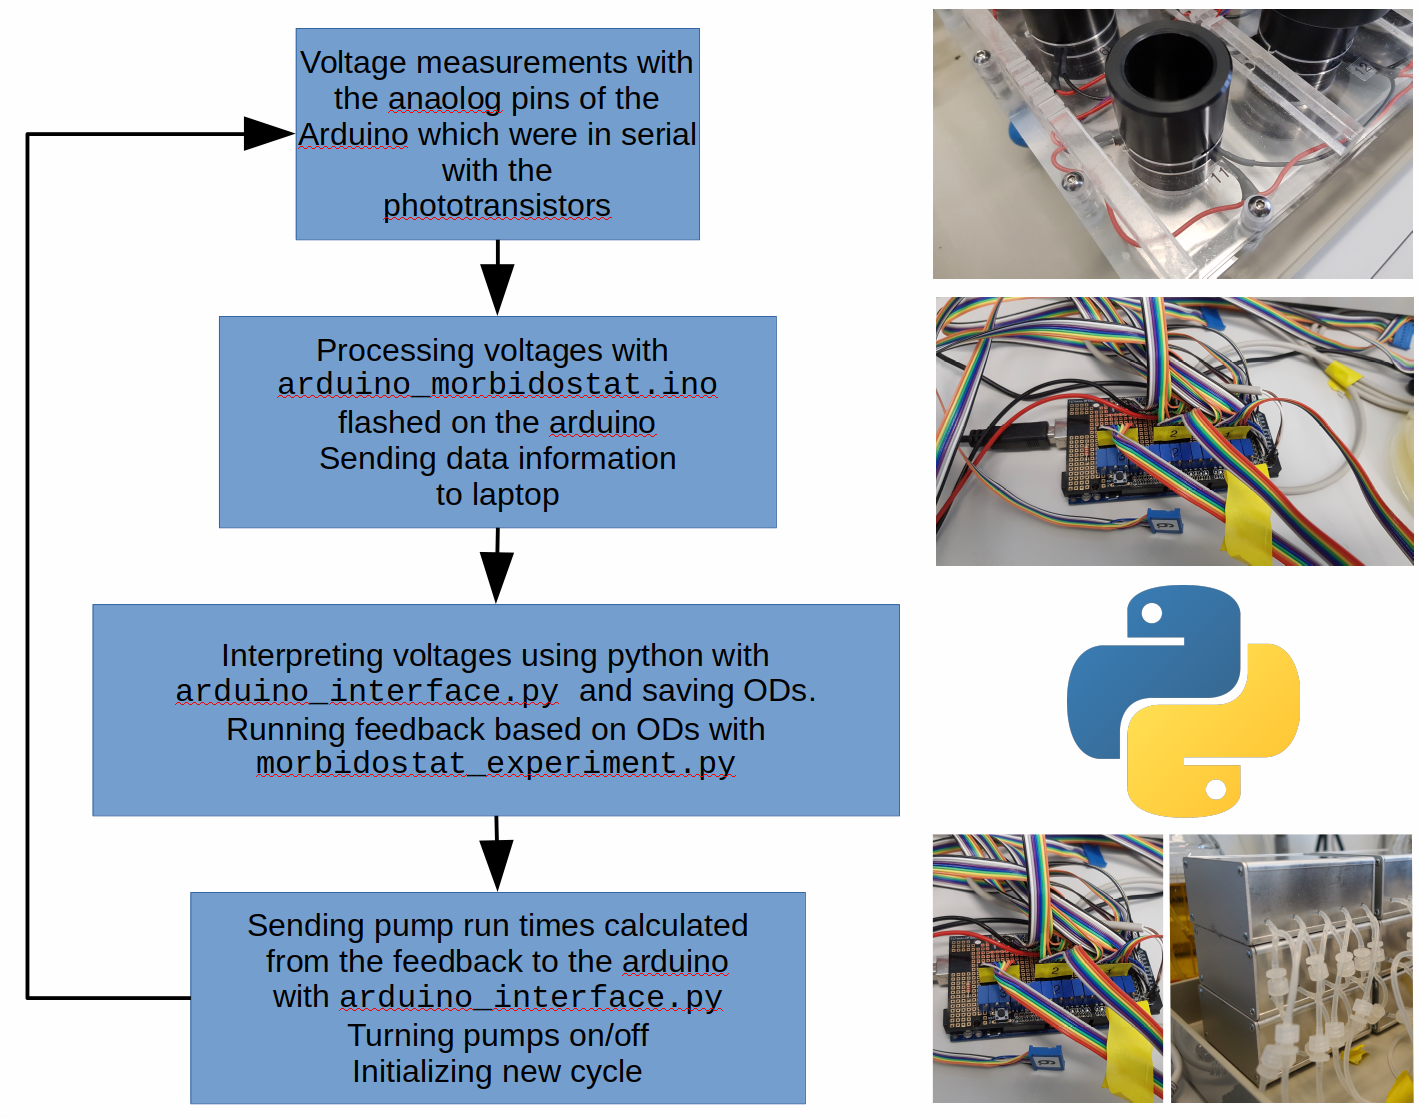
\includegraphics[scale=0.25]{flowchart.png}
	\caption{Overview of one cycle from the continuous mode of the morbidostat.}
	\label{figure:flowchart}	
\end{figure}

\subsubsection{Feedback of the continuous mode} 
The feedback determined how strongly the cultures were inhibited. This feedback was based on the relative difference between the averaged ODs of the current cycle and the averaged ODs of a past cycle. We called the average ODs of a cycle final\_OD and the relative difference between two final\_ODs \textDelta OD. 
\begin{center}
	$\Delta OD = (final\_OD_{x_{cycles\_back}} - final\_OD_{current\_cycle})/x$
\end{center}
As shown in in Figure \ref{figure:feedback} the feedback did several comparisons before calculating an appropriate dose of antibiotics. As a first step it checked if \textDelta OD was positive or negative. A negative \textDelta OD implied that the bacteria were dying. In order to prevent complete sterilization, media was injected in this case. \\
When \textDelta OD was positive the bacteria were growing. Antibiotics were only injected if the bacteria reached a certain OD called drug\_dilution\_threshold. Therefore, the next comparison as visible in Figure \ref{figure:feedback}, was whether or not the final\_OD was higher or smaller than this threshold. If the final\_OD was smaller no fluids were injected.
However when final\_OD was bigger than the threshold calculation of the appropriate dose was initialized.
The calculation itself was split up into two equations. One equation, mainly important at the beginning of the morbidostat experiments, was used to approximate the MIC of the strains. This was done by simply adding a fraction of the MIC for every cycle. After the MIC was reached this equation was ignored and from now on the second equation determined the injected concentration. This equation multiplied the current drug concentration in the vials by the \textDelta OD which resulted in how much the drug concentration in the vial was increased.
The goal of the feedback was that a certain OD called target\_OD was approximated in every vial. In order to do so we divided the second equation by this target\_OD. Now if a small target\_OD was chosen the increased concentration was divided by a small value causing a higher injected concentration. If target\_OD was set to a high value the divided outcome was smaller. 

\begin{figure}
	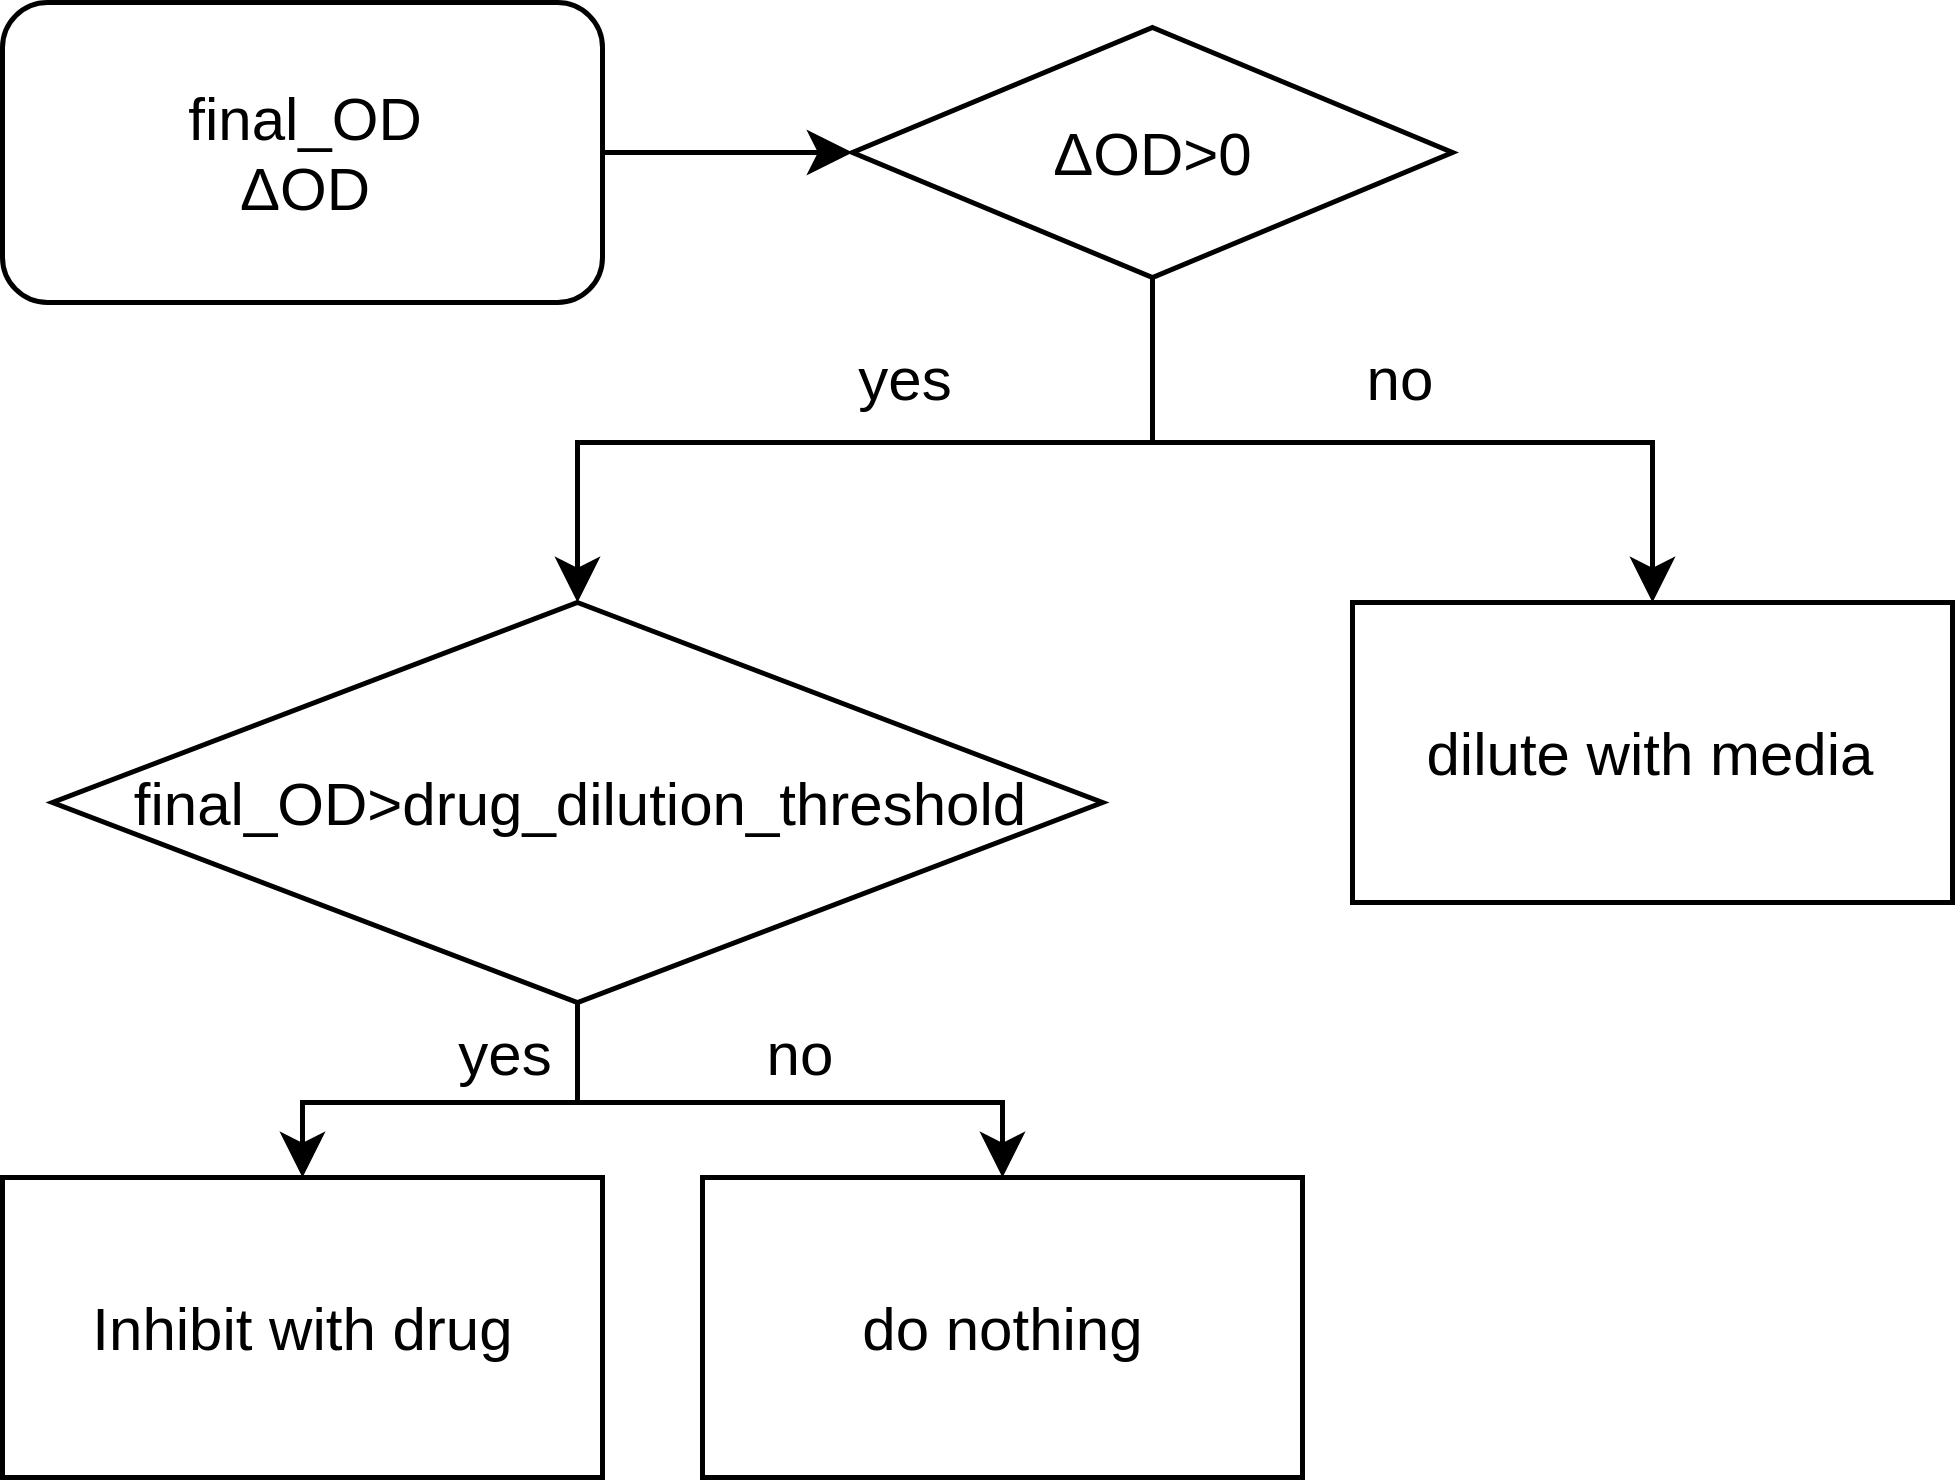
\includegraphics[scale=0.13]{feedback.png}
	\caption{Schematic overview of decisions involved in the feedback}
	\label{figure:feedback}
\end{figure}

\subsection{Hardware calibration}
\subsubsection{OD and pump calibration}
For calibrating the OD measurements an overnight culure with K12 XL1 blue E. coli was inoculated in 5 ml 9/10 $H_2O$ and 1/10 LB media (also referred as diluted media). The next day the overnight culture was diluted 1/200 in 50 ml diluted media. After a few hours of day culturing following OD standards were prepared with 18 ml diluted media in the vials for the morbidostat: 0.01 0.021 0.042 0.107 0.192 0.278\\
Then every vial with a certain OD was placed in every vial holder. With the function calibrate\_OD from the \href{https://github.com/nahanoo/ESBL\_project/}{morbidostat\_experiment.py}, a voltage measurement was done for every OD standard and every OD measuring unit. The result of this function was a linear equation which translated the voltages to ODs. \\
\begin{figure}
	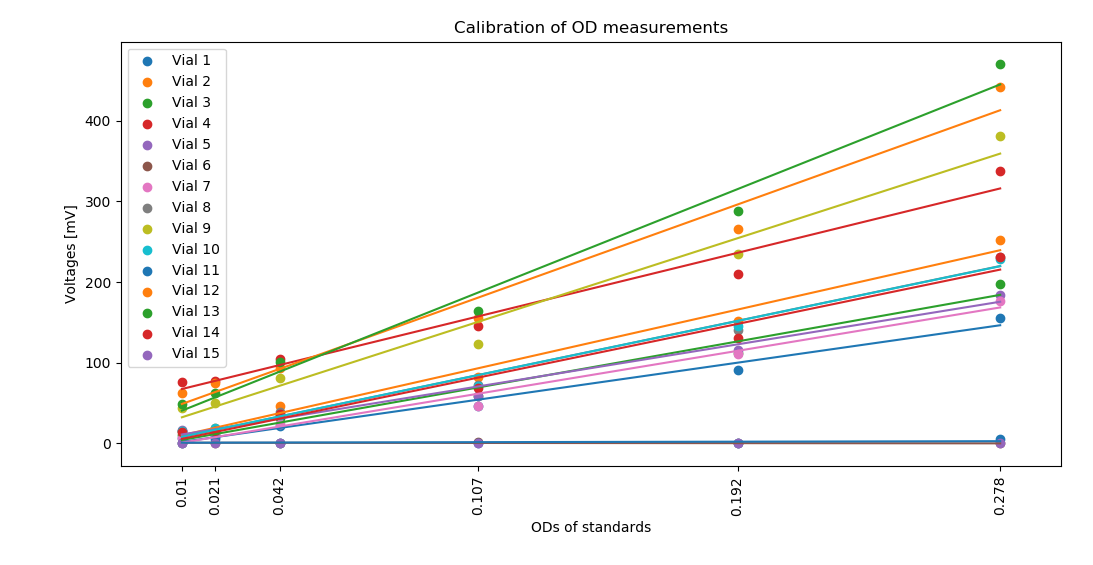
\includegraphics[width=1\textwidth]{od_calibration.png}
	\caption{Calibration of OD measuring units, with the OD standards on the x-axis and the measured voltages on the y-axis. The line represents the calculated linear equation. The units of vial 5 and 15 were not working.}
\end{figure}
For calibrating the pumps the function calibrate\_pumps from the\href{https://github.com/nahanoo/ESBL\_project/}{morbidostat\_experiment.py} was executed. The weight of every empty vial had to be entered and the function turned on every specified pump for 100 seconds. Afterwards the weight of the vials was entered again and the function calculated the flow rate for the specified pumps. 
\label{section:OD_calibration}

\section{Forcing \textit{ESBL E. coli} to evolve resistance with the morbidostat}
We decided to produce ESBL \textit{E. coli} strains with \textit{E. coli} K-12 MG1655 and the ESBL genes from the sample collection of the University Hospital of Basel (see Section \ref{section:samples}. \textit{E. coli} K-12 is a model organism which does not colonize the human intestine \cite{k-12}. Compared to working with the strains from the University Hospital of Basel, handling K-12 strains is much safer.  
\subsection{Producing ESBL \textit{E. coli} clones}
Three different ESBL \textit{E. coli} strains were produced by our collaborators by gibson cloning. We derived the ESBL gene sequences and the upstream sequence up to the previous gene from samples of the University Hospital of Basel. In particular we extracted the sequences from patient 25 sample 1 and patient 33 sample 1. 
For each sequence an identifier was created which also acted as the identifier of the strain.

\begin{table}[H]
	\begin{tabular}{|c c|}	
		\hline
		Plasmid ID & ESBL \\
		\hline
		pEU22 & CTX-M-1 \\
		\hline
		pEU23 & OXA \\
		\hline
		pEU26 & OXA \\
		\hline
	\end{tabular}
	\label{table:plasmid}
	\caption{Produced plasmids}
\end{table}
\subsection{Gibson cloning}

\subsection{Morbidostat experiments}
\begin{figure}
	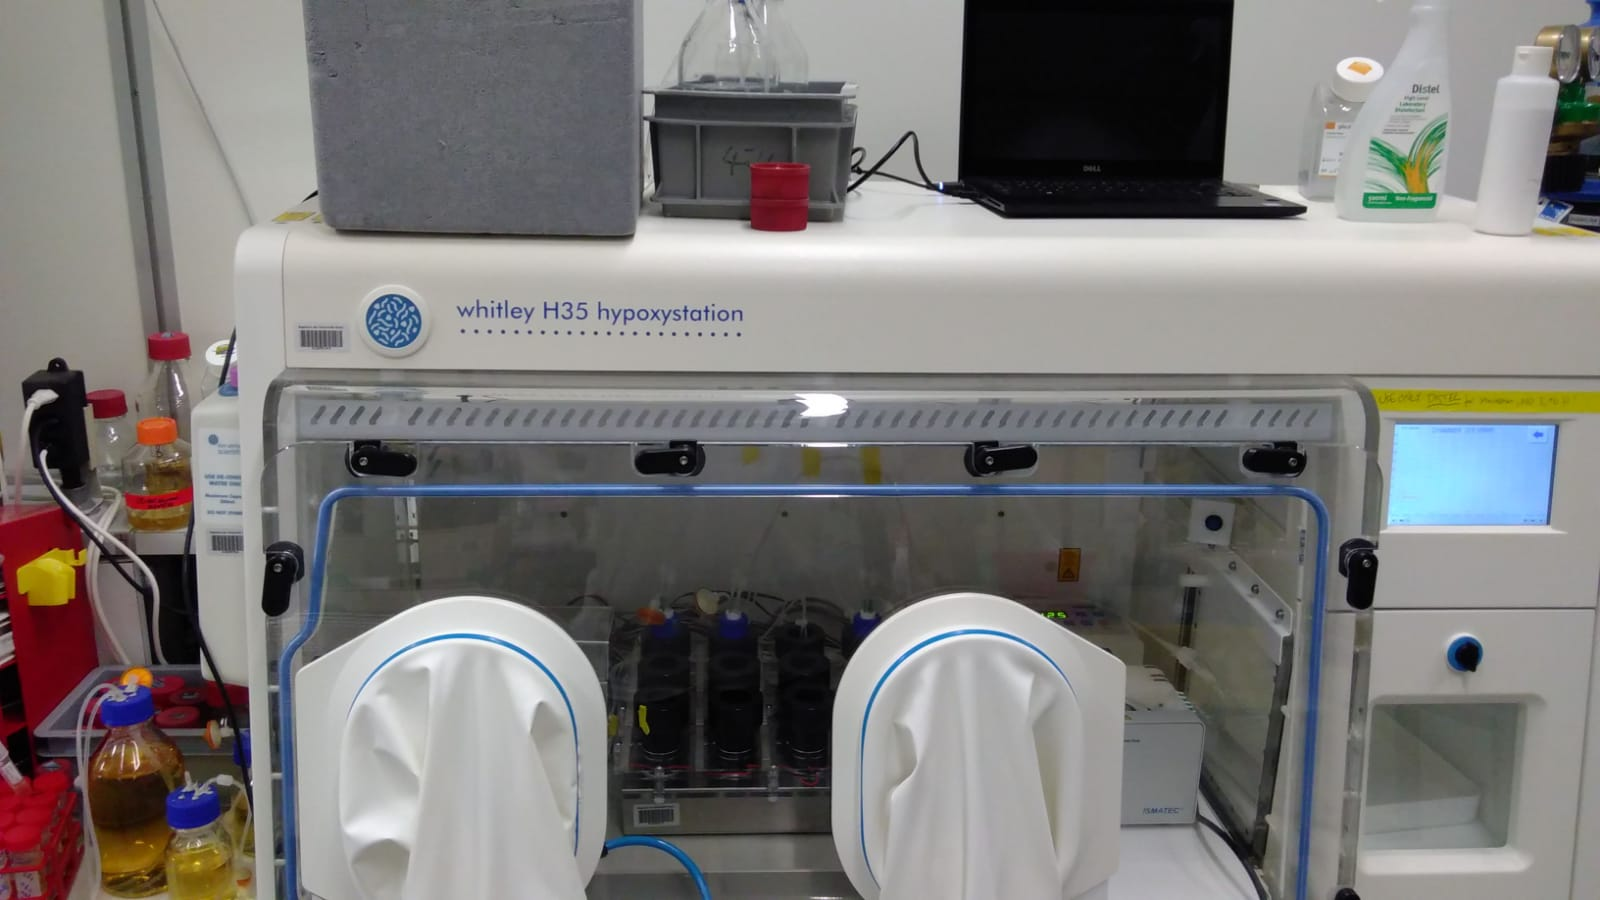
\includegraphics[width=0.5\textwidth]{hypoxi-station.jpeg}
	\caption{Morbidostat setup inside the hypoxi-stationi. Media and drug bottles are placed outside on the left side. Waste bottle is placed underneath the hypoxi-station in a sealed container.} 
\end{figure}
We ran two morbidostat experiments with the ESBL \textit{E. coli} strains. The morbidostat was set up inside the hypoxi-station in a bio safety lab 2. Placing the morbidostat in the hypoxi-station allowed us to culture at 37 \degree C while increasing the safety and controlling the $N_2$ and $CO_2$ composition. Before we started culturing with the morbidostat, the MIC of the ESBL \textit{E. coli} strains was measured and the morbidostat was sterilized.
\subsubsection{MIC determination}
We inoculated every ESBL \textit{E. coli} strain in 5 ml of MHB media and cultured the suspension over night at 37 \degree C. The next day a 1/200 dilution in 20 ml MHB was prepared for every suspension and cultured for a few hours at 37 \degree C. In the meanw while we prepared a cefepime solution with a concentratio of 2.048 mg/ml. The growth of the diluted cultures was constantly monitored by measuring the OD. When the OD of the diluted culture was at 0.08, a 1/100 dilution of every culture was prepared. From this dilution 100 \textmu L were pipetted in every well of a 96 well expect in the wells from the last column of the plate. To every well 100 \textmu L of MHB were added to every well. As a next step 100 \textmu L from the prepared drug solution was added to the first column of the plate. Then 100 \textmu L from this column was transferred to the next column and mixed. This was repeated until the third last column was reached. The second last column acted as a growth control of the strains and the last column As a negative control. We incubated the plates for 16 hours at 37 \degree \space on a shaker. To get an idea how many cells were used for the MIC determination $10^{-3}$ and $10^{-5}$ dilutions of the 1/100 diluted cell cultures were plated on LB plates.\\
After 16 hours the OD of every well was measured using a plate reader. The smallest concentration which inhibited the growth was determined as the MIC. 
\label{section:mic_determination}

\subsubsection{Sterilization of the morbidostat}
In order to prevent biofilm formation and contamination of our vials we sterilized the entire setup using two different disinfectants.
Bottles, vials, tubing and luer connections were autoclaved. Sterile vials were connected to the tubes and the computer controllable pumps were connected to 1 L of 3 \% citric acid stord in a sterile bottle with sterile tubing. All the tubing going to the vials was flushed with the desinfectant over one hour. The waste pump was turned on leading to disinfection of the tubes connected to the sterile waste bottle. After that the tubing was flushed with 1 L of sterile water. We repeated this procedure but this time using 3 \% of bleach as disinfectant.
\label{section:sterilization}

\subsubsection{Culturing with the morbidostat}
We ran two morbidostat experiments with the ID 01 and 02 with the ESBL \textit{E. coli} strains. For every experiment we prepared over night cultures of the ESBL \textit{E. coli} strains in 3 ml diluted media with 3 \textmu L kanamycine.\textit{E. coli} K-12 MG1655 was cultured over night in 3 mL diluted media. The over night cultures were diluted 200 fold the next day and cultured for a few hours. From those cultures, 200 \textmu L were transferred into sterile vials containing 18 mL diluted media. We prepared two different antibiotic concentrations which were connected to the pumps. We prepared a concentraton of of 9 \textmu g/ml cefepime in 1 L diluted media as a low concentrated antibiotic solution. For the high concentrated solution we prepared a cefepime concentration of 21 \textmu g/mL in 1 L diluted media. The morbidostat experiment were initialized with a target\_OD of 0.12, and a dilution factor of 0.91. Every ESBL \textit{E. coli} strain was cultured at least three times with the continuous mode. Additionally we cultured every ESBL \textit{E. coli} strain with the fixed\_OD mode. The temperature inside the hypoxi-station was set to 37 \degree C. The $O_2$ level was fixed to 10 \% and $CO_2$ fixed to 5 \%. \\
As resistance evolved the antibiotic concentrations of the bottles were changed. We checked which concentration was necessary to strongly inhibit the cultures and passed this values as new MIC the python scripts. New cefepime concentrations which were 3 fold and 7 fold higher than the newly determined MIC were prepared and connected. We changed the antibiotic concentrations of the bottles approximately every third day. If the suspension in the vials was extremely milk caused by dead cells we transferred 200 \textmu L of the suspension to a new sterile vial containing 18 ml diluted media.  \\
During both experiments we took daily samples by opening the vial in the hypoxi-station and transferring 1 mL to an eppendorf tube. The collected samples were centrifuged ad 13'000 rpm for 10 minutes and resuspended in 200 \textmu L LB containing 20 \% glycerol. Those suspensions were frozen at -80 \degree C.\\

\subsection{Analysis of the morbidostat samples}
\subsubsection{Illumina and Nanopore sequencing}
We handed the stocks of the cloned ESBL \textit{E. coli} strains and K-12 MG1655 to to our collaborators of the University Hospital of Basel were they were sequenced on a MiSeq-Illumina system (see Section \ref{section:illumina}).
Furthermore, we passed the stocks for Illumina sequencing of the last sample day of every vial form the 01 experiment. 
From the 02 experiment we selected the stocks from vial 3,4,5,7 and 8 from the third sample day and the stocks from every vial of the last sample day for Illumina sequencing. Every stock that we handed over for Illumina sequencing was stroke out on LB plates containing kanamycin except K-12 MG1655 was stroke out on a LB plate.
We sequenced the cloned ESBL \textit{E. coli} stocks and K-12 MG1655 with ONT. For DNA extraction we inoculated 3 mL LB containing 1 \% kanamycin with the ESBL \textit{E. coli} stocks. K-12 MG1655 was inoculated in 3 mL LB. The suspensions were cultured over night. The DNA of the resulting over night cultures was extracted following the protocol of the DNeasy Blood \& Tissue Kit (50). The extracted DNA was sequenced with a MinION as described in Section \ref{section:nanopore_sequenicng}. 

\subsubsection{Contamition analysis}
On the plates where we stroke out every stock that we handed over for Illumina sequencing we saw colonies which had a different shape than \textit{E. coli}. Therefore, we had the suspicion that some stocks were contaminated. Because we had Illumina sequencing data for every stock we could identify the contamination by blasting a few reads \cite{madden_blast_2003}. This revealed that the contamination was \textit{Bacillus cereus}. To identify which samples were contaminated, all the Illumina short-reads from every stock  were mapped to a \textit{Bacillus cereus} reference genome obtained from NCBI \cite{noauthor_bacillus_nodate} and the ESBL \textit{E. coli} reference genome produced with hybrid-assembling.

\subsubsection{Identifying mutations in morbidostat samples}
The sample series from the morbidostat experiments where analyzed following the bioinformatical pipeline described in Section \ref{section:pipeline}. 
\section{Bioinformatic pipeline for identifying mutations in ESBL \textit{E. coli} accumulated by evolving resistance against cefepime}
\label{section:pipeline}
\begin{figure}
	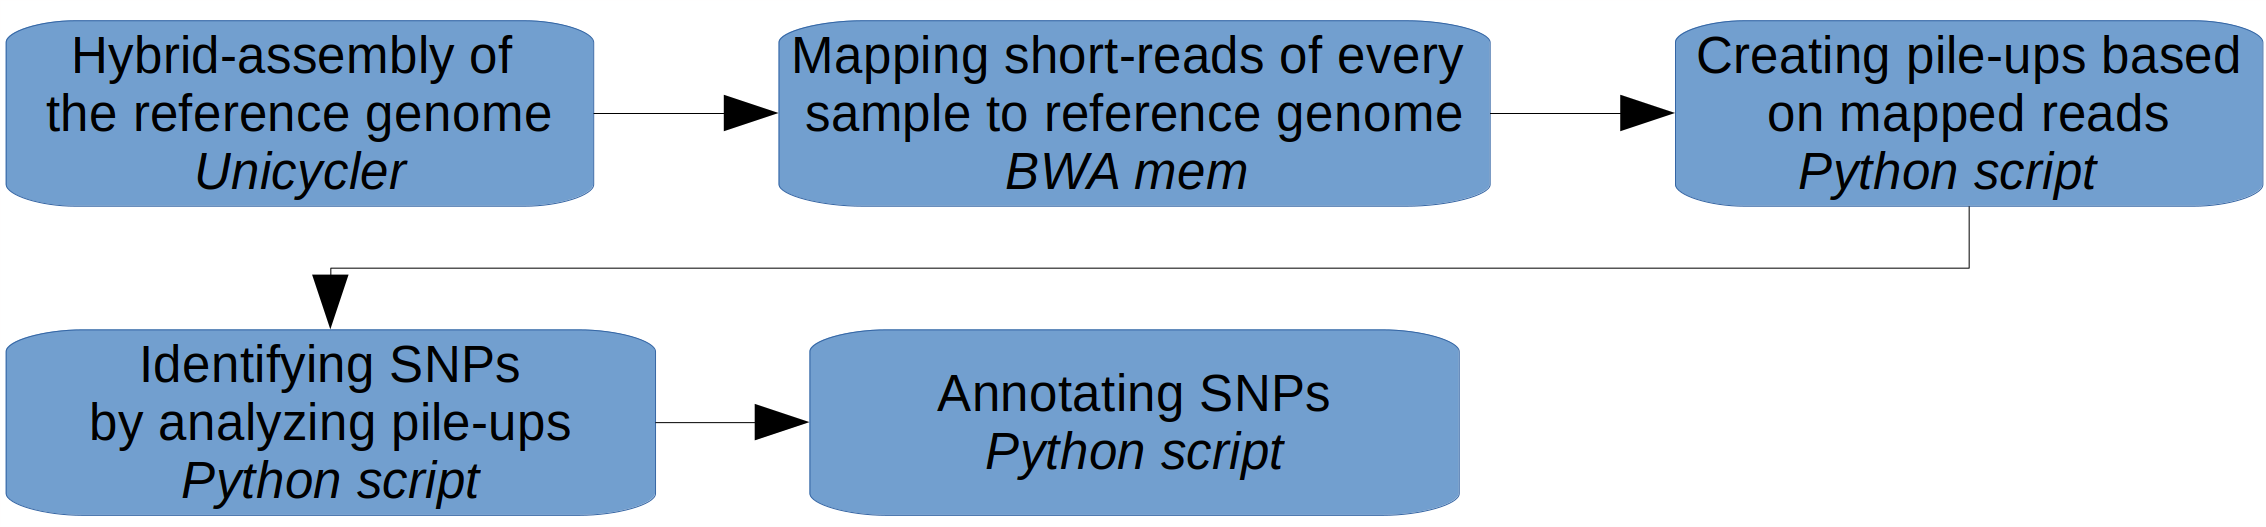
\includegraphics[width=0.9\textwidth]{pipeline.png}
	\caption{Bioinformatic pipeline used for the identification of mutations and affected genes/promotors.}
	\label{figure:pipeline}
\end{figure}
We established a bioinformatic pipeline which allowed us to identify mutations which accumulated by evolutionary pathways while ESBL \textit{E. coli} strains changed their phenotype from susceptible to resistant to cefepime. Thise pipeline was based on sequencing data coming from multiple samples which were taken while resistance evolved. Samples taken along such a pathway are also referred as sample series. The steps of the pipeline are shown in Figure \ref{figure:pipeline}.

\subsection{Creating a reference genome with annotation} 
The first step was to de novo assemble the genome of the sample with the lowest cefepime MIC of a sample series. We called the whole-genome assembly of this sample reference genome. For whole-genome assembling we used Unicycler \cite{wick_unicycler:_2017} as an assembler. With Unicycler \cite{wick_unicycler:_2017} we combined long-read sequencing data produced with Oxford Nanopore Technologies (ONT) and short-read Illumina sequencing into a hybrid-assembly. ONT sequencing was done by ourselves, Illumina sequencing by our collaborators of the University Hospital of Basel.  

\subsubsection{ONT sequencing}
For ONT sequencing the library was prepared with a ligation sequencing kit (LSK-108) followed with the native barcoding expansion kit. This allowed barcoding of multiple samples and loading all of them on a single flow cell (FLO-MIN106D). As a sequencing device we used the MinION from ONT. \\
As a fist step each DNA isolate was diluted to a concentration of 1 \textmu g/\textmu l in 50 \textmu L nuclease free water (NFW). For end-repairing the DNA 7 \textmu L NEBnext Ultra II Endrepair/dA-tailing enzyme mix were added to each
sample and incubated at 20\degree C for 5 min and at 65\degree C also for 5 min. After this step every sample was cleaned up by adding 60 \textmu of AMPure XP beads. The beads were incubated with the samples for 5 miuntes ona a rotor and then removed on a magnetic rack. Every sample was washed with 200 \textmu L 70\% ethanol which was repeated once. The ethanol was removed and every sample was suspended in 25 \textmu L NFW. 2.5 \textmu L of each barcode plus 25 \textmu L of Blunt/TA ligase was added to each sample and incubated for 10 minutes. All the samples were pooled and 500 \textmu of AMPure XP beads were added. After incubating the pooled sample for 5 minutes on the rotor the sample was washed again twice with 70 \% ethanol. All the DNA was eluted in 51 \textmu L NFW. The final sample was diluted to a concentration of 35 ng/\textmu L. Then for adapter ligation 20 \textmu L BAM, 30 \textmu L Ultra II ligation master mix and 1 \textmu L enhancer were added. After 10 minutes of incubation, 40 \textmu L AMpure XP beads were added and incubated on the rotor for 5 minutes. The supernatant was removed on the magnetic rack and the DNA was washed twice with ABB. The DNA was eluted and incubated for 10 minutes in 15 \textmu L ELB. Finally the library was prepared by mixing 15 \textmu L of eluted DNA in ELB with 25.5 \textmu L LLB and 35 \textmu L RBF. The resulting library was loaded on the flow cell, which was primed before with a mixture of 480 \textmu L RBF  and 520 \textmu L of NFW. The sequencing run was started and simultaneously base-called with Albacore.
\label{section:nanopore_sequenicng}

\subsubsection{Illumina sequencing}
The DNA from the samples was isolated using the EZ1 DNA tissue kit on an EZ1 Advanced XL robotic system (Qiagen). The library for the sequencing was prepared using the Nextera XT library preparatino kit (Illumina) and the resulting library was sequenced on a MiSeq Illumina platform \cite{nanopore}. The reads produced with Illumina were trimmed with Trim Galore \cite{noauthor_babraham_nodate}.
\label{section:illumina}

\subsubsection{Annotating the reference genome}
Every reference genome was annotated with prokka (v.1.12) which produced a genbank file for every reference genome \cite{seemann_prokka:_2014}. Prokka first searches a core set of well characterized protein using BLAST+ and then compares reading frames to a database derived from UniProtKB \cite{seemann_:zap:_2019}. Additionally promotor regions were identifed using the promoter prediction tool PePPER \cite{pepper}. PePPER is a tool which takes whole-genomes as an input and predicts promotor sequences. Those sequences were mapped against the reference genome using graphmap \cite{sovic_fast_2016}. Furthermore a promotor data base hosted on EcoCyc was used. This data base contains around 3800 experimentally validated promotors for \textit{E. coli}\cite{noauthor_smarttable_nodate}. The sequences from this database were downloaded and mapped against the reference genome with graphmap aswell \cite{sovic_fast_2016}. 
\label{section:annotatiion_ref}

\subsection{Mapping Illumina sequencing data of the sample series to the reference genome}
As a second step of the pipeline the short-read Illumina sequencing data of every sample was mapped against the reference genome of the sample series. Mapping to the reference genome was done with BEW mem \cite{li_fast_2009}. This resulted in a bam file for every sample of the series. Mapping all the Illumina reads provided us the inofrmation which base was present in every Illumina read mapped to a certain position to the reference genome. If the most abundant base of all Illumina reads at a certain position is different than in the reference genome a mutation was present. To make this information more accessible we calculated pile-ups as a third step of our analysis. 

\subsection{Calculating pile-ups}
Pile-ups are count matrices which store which base is present how many times at a certain position considering every mapped Illumina read. In order to produce those pile-ups we used a script called \href{https://github.com/nahanoo/ESBL\_project/pileup.py}{pileup.py}. This script extracted the base counts by going through every position of the bam-file from a sample. Pile-ups were calculated for every sample of a series and all the pile-ups stored in a matrix stack. Next to identification of the most abundant base, pile-ups also allowed us to easily calculate base frequencies and the coverage which was easily comparable within a series because all pile-ups were stored in a matrix stack.

\subsection{Identification of mutations} 
We identified mutations by comparing the most abundant base at every position of the matrix-stack with a script called \href{https://github.com/nahanoo/ESBL\_project/pileup.py}{analysis\_modular.py}. If the most abundant base varied between the samples of the matrix-stack a single-nucleotide polymorphism (SNP) was identified. For the rest of the pipeline only mutations were included where the coverage was at least 30 and the base frequency at least 0.8.

\subsection{Identifying genes and promotors affected by mutations}
As a last step of the pipeline we checked if annotation was available for every found mutation. As described in section \ref{section:annotatiion_ref} genes and promoters were identified for every reference genome. \\
For checking if a SNP affected a gene, we analyzed the genbank file with biopython \cite{cock_biopython:_2009}. We checked if a mutation was located between a start and an end position of a gene. For checking if a SNP affected a promotor region we analyzed the bam-files which were created with the promoter sequences coming from PePPER and EcoCyc (see \ref{section:annotatiion_ref}). We checked if a SNP was loacted between a start or end positon of a mapped promotor sequence. 

\chapter{Results}
\section{Analyzing ESBL E. coli isolates from patients
of the University hospital Basel}
\subsection{Sample selection}
The sample collection consisted of 65 samples screened positive for ESBL genes coming from 34 patients. An identifier was created for each sample consisting of the patient number and the sample number. Sample numbers chronologically increased meaning that sample 0 was the first sample collected from a patient. From the 34 patients we had to select for patients wich were suitable for our analysis. Obviously multiple samples per patient were necessary which was not the case for 15 patients. In order that SNPs could be identified which were likely associated with resistance it was necessary that the samples collected from one patient were the same ESBL E. coli strain. By building a phylogenic tree of all the samples we could check how closely related different samples were.  

\subsubsection{Pylogeneic analysis with panX}
\begin{figure}
	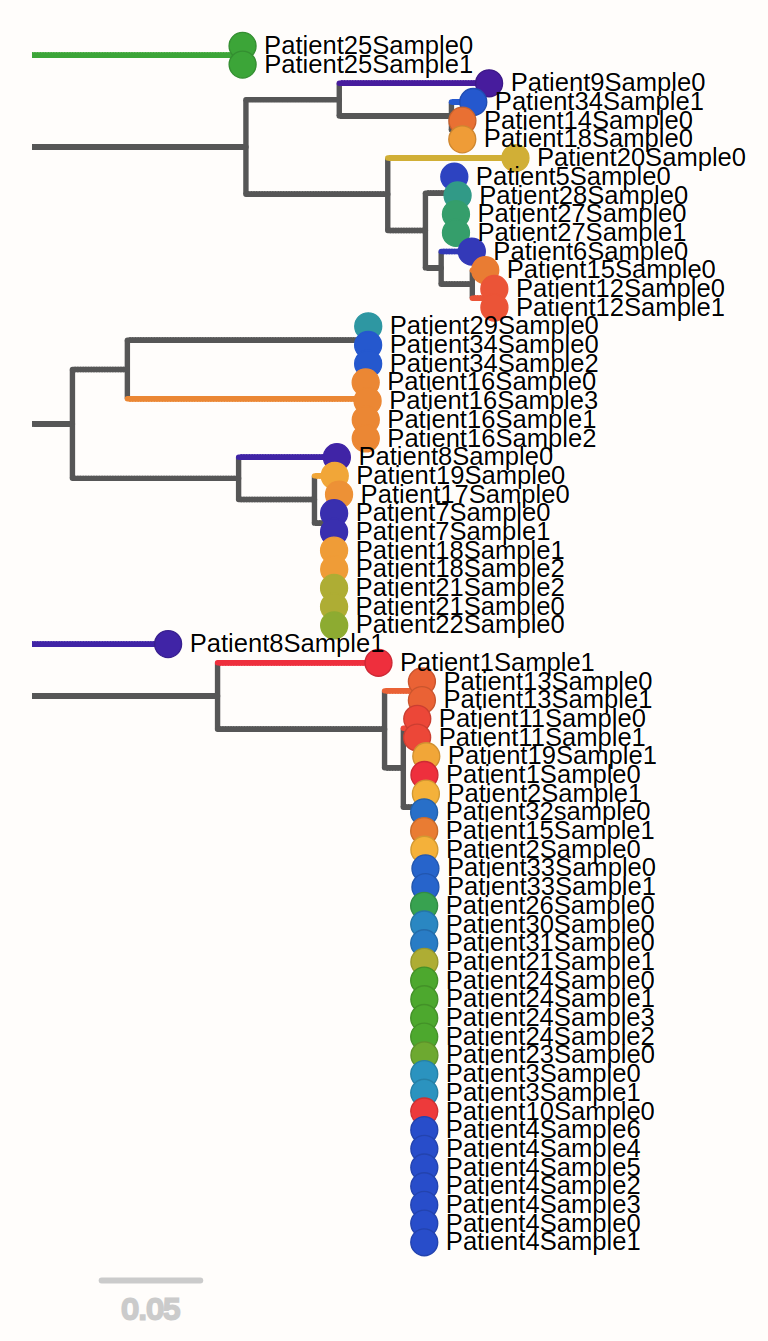
\includegraphics[scale=0.2]{181205_panXtree_overview.png}
	\caption{Phylogenic tree built wihn panX. The samples are colored by the patient.}
	\label{figure:panX}
\end{figure}
Only patients could be used for the analysis where every sample mapped on the same branch on the phylogenetic tree created with PanX. If that was the case the samples shared the identical core genomes. 
Samples of one patient mapping on different branches imply that their core genome differed and they were different strains. Therefore the patient was infected with different strains over the sample period which made it impossible for us to identify SNPs potentially involved in the resistance mechanism. \\
From the 19 patients with multiple samples 7 patients had samples which mapped on different branches. This is visible in Figure \ref{figure:panX}. For example patient 15 had two samples which mapped on two different clades of the tree.
Those 7 patients had to be excluded from the analysis as well. \\
It's also visible in Figure \ref{figure:panX} that some samples from different patients map on the same branch. This tells us, that some patients were infected by the same strain coming probably from the same outbreak within the hospital. On the other hand patient 25 has two samples which map on a separate clade of the pyhlogenic tree. This indicates that this patient most likely got infected outside the hospital.  

What also reduced the patients which could be used for the analysis was that not all of them had a significant increase or decrease of the MIC for cefepime or ceftazidime. Since those MIC were determined by a 2-fold dilution series it was not enough when the concentration doubled over time. This reduced the selection to 5 patients. The meta data and the MIC for those patients are shown in Table \ref{table:samples_overview}. 
\begin{table}
	\begin{tabular}{|c c c c c|}	
		\hline
		Accession & Sample date & MIC Cefepim & MIC Cefepim Sandra & Ceftazidim \\ [0.5ex]
		\hline\hline
		\rowcolor{LightCyan}
		Patient12Sample0 & 9.9.14 & 4 & 16 & 0.75 \\
		Patient12Sample1 & 5.12.14 & 12 & 32 & 2 \\
		\hline
		\rowcolor{LightCyan}
		Patient16Sample0 & 22.6.12 & 8 & 32 & 2\\
		Patient16Sample1 & 18.7.13 & 48 & 64 & 8\\
		Patient16Sample2 & 1.11.13 & 32 & 32 & 12\\
		\hline
		\rowcolor{LightCyan}
		Patient24Sample0 & 02.05.11 & 4 & 16 & 1.5\\
		Patient24Sample1 & 08.15.11 & 16 & 32 & 1.5\\
		Patient24Sample2 & 11.28.11 & 3 & 8 & 1\\
		\hline
		Patient25Sample0 & 15.4.11 & 64 & None & 192\\
		\rowcolor{LightCyan}
		Patient25Sample1 & 22.8.11 & 6 & 4 & 6\\
		\hline
		Patient33Sample0 & 26.9.14 & 24 & None & 16 \\
		\rowcolor{LightCyan}
		Patient33Sample1 & 29.1.15 & 1 & 2 & 1.5\\
		\hline
	\end{tabular}
	\caption{Those patients have been selected because their samples differ significantly in MIC and mapped on the same branch in panX. The samples which are stained in cyan were chosen for building the reference genome.}
	\label{table:samples_overview}	
\end{table}

\subsection{Sequencing and assembling}
Ever sample shown in Table \ref{table:samples_overview} was successfully sequenced with a MinION from Oxford Nanopore Technologies. From each patient a reference genome was successfully built for the sample with the lowest MIC. The selected sample for building the reference genome is shown stained in cyan in Table \ref{table:samples_overview}. Note that for patient 24 sample 0 was selected even though technically sample 2 has lower MICs. But since the MIC from those samples are very similar we decided to choose sample 0 because it was collected the earliest. 

As shown in Table \ref{table:sequencing} the lowest coverage for a sequenced sample which was used to built a reference genome was 73. All the other samples had a coverage of higher than 200, but even 73 is more than sufficient. The last column of Table \ref{table:sequencing} shows how many contigs were detected by Unicycler. Note that a hybrid assembly was used to build the reference genome, which means that the long-reads from Nanopore were supplemented with short-reads from Illumina. 
\begin{table}
	\begin{tabular}{|c c c c|}	
		\hline
		Accession & Total gigabases sequenced & Coverage & Assembled in n contigs \\ [0.5ex]
		\hline\hline
		Patient12Sample0 & 0.39 & 73 & 6 \\
		\hline
		Patient16Sample0 & 1.11 & 207 & 3 \\
		\hline
		Patient24Sample0 & 1.81 & 336 & 17\\
		\hline
		Patient25Sample1 & 1.82 & 338 & 12\\
		\hline
		Patient33Sample1 & 1.24 & 231 & 6 \\
		\hline
	\end{tabular}
	\caption{Total sequenced bases and resulting coverage for every sample which was chosen for building a reference genome. The coverage was calculated by assuming the genome size of E. coli is 5.4 megabases. the last column displays into how many contigs the genome was devided by the assembler Unicycler. }
	\label{table:sequencing}	
\end{table}

\subsection{SNPs}
Mapping all the short-reads from one patient to the according reference genomes revealed about 100 SNPs for all patients. Those SNPs had a short-read coverage of at least 30 and a minimum base frequency of 0.8. \\
Only SNPs with annotation are presented in the following tables. All the tables with SNPs with gene annotation share the same structure. The first column describes in which sample the SNP was identified. The columns "gene" and "product" describe what gene and transcribed protein is affected by the SNP. The last column shows at which position of the gene the SNP caused a change of the amino acid. The first amino acid is the one found in the reference sample. The second amino acid is the changed amino acid in the resistant sample caused by the SNP. 
Only for patient 16 SNPs were found with promoter annotation.
The SNPs with no annotation are listed for all patients in the supplementary (see Section \ref{section:snps_with_no_annotation}) 
\subsubsection{Patient 12}
For patient 12 no SNPs with annotation were found. In total 4 SNPs were identified for this patient.

\subsubsection{Patient 16}
In Table \ref{table:pat16_snp_annotated} every SNP for this patient is shown where a gene annotation was found. All of the SNPs for this patient were found on the chromosome. In total we detected 46 SNPs for this patient. 
\begin{table}[]
	\begin{tabularx}{\linewidth}{|cccLLL|}
		\hline
		\#SNP & Contig & Position & \multicolumn{3}{l|}{Nucleotide in Sample:} \\
		&        &          & 0     & 1     & \multicolumn{1}{l|}{2}    \\ \hline
		1     & 0      & 109928   & C     & A     & \multicolumn{1}{l|}{C}    \\ \hline
		2     & 0      & 1895312  & A     & C     & \multicolumn{1}{l|}{A}    \\ \hline
		3     & 0      & 2101128  & G     & -     & \multicolumn{1}{l|}{-}    \\ \hline
		&        & 2101129  & C     & -     & \multicolumn{1}{l|}{-}    \\ \hline
		&        & 2101130  & A     & -     & \multicolumn{1}{l|}{-}    \\ \hline
		4     & 0      & 2375277  & C     & T     & \multicolumn{1}{l|}{C}    \\ \hline
		5     & 0      & 3797984  & A     & G     & \multicolumn{1}{l|}{A}    \\ \hline
		6     & 0      & 4200032  & T     & C     & \multicolumn{1}{l|}{T}    \\ \hline
		7     & 0      & 4353560  & G     & C     & \multicolumn{1}{l|}{G}    \\ \hline
		8     & 0      & 5112127  & G     & T     & \multicolumn{1}{l|}{G}    \\ \hline
		9     & 0      & 55597    & A     & G     & \multicolumn{1}{l|}{G}    \\ \hline
		10    & 0      & 922702   & G     & A     & \multicolumn{1}{l|}{G}    \\ \hline
		11    & 0      & 1133762  & C     & T     & \multicolumn{1}{l|}{T}    \\ \hline
		12    & 0      & 1549518  & T     & G     & \multicolumn{1}{l|}{G}    \\ \hline
		13    & 0      & 2016331  & A     & C     & \multicolumn{1}{l|}{A}    \\ \hline
		14    & 0      & 2101129  & C     & -     & \multicolumn{1}{l|}{-}    \\ \hline
		&        & 2101130  & A     & -     & \multicolumn{1}{l|}{-}    \\ \hline
		15    & 0      & 3920934  & A     & G     & \multicolumn{1}{l|}{A}    \\ \hline
		16    & 0      & 4333944  & C     & T     & \multicolumn{1}{l|}{T}    \\ \hline
		17    & 0      & 4459680  & C     & -     & \multicolumn{1}{l|}{C}    \\ \hline
		&        & 4459681  & C     & -     & \multicolumn{1}{l|}{C}    \\ \hline
		18    & 0      & 4459684  & G     & -     & \multicolumn{1}{l|}{G}    \\ \hline
		&        & 4459685  & A     & -     & \multicolumn{1}{l|}{A}    \\ \hline
		&        & 4459686  & A     & -     & \multicolumn{1}{l|}{A}    \\ \hline
		&        & 4459687  & G     & -     & \multicolumn{1}{l|}{G}    \\ \hline
		&        & 4459688  & A     & -     & \multicolumn{1}{l|}{A}    \\ \hline
		&        & 4459689  & G     & -     & \multicolumn{1}{l|}{G}    \\ \hline
		19    & 0      & 4459692  & A     & -     & \multicolumn{1}{l|}{A}    \\ \hline
		&        & 4459693  & G     & -     & \multicolumn{1}{l|}{G}    \\ \hline
		20    & 0      & 4459695  & G     & -     & \multicolumn{1}{l|}{G}    \\ \hline
		21    & 0      & 4459697  & T     & -     & \multicolumn{1}{l|}{T}    \\ \hline
	\end{tabularx}
\end{table}
\begin{table}[]
	\begin{tabularx}{\linewidth}{|ccLLccc|}
		\hline
		\#SNP & Gene          & Product                                  & Type and position in gene      & \multicolumn{3}{l|}{Amino acid in Sample:} \\
		&               &                                          &                        & 0   & 1               & 2               \\ \hline
		1     & \textit{ortT} & Orphan toxin OrtT                        & Missense, 44           & P   & T               & P               \\ \hline
		2     & \textit{scrY} & Sucrose Porin                            & Missense, 104          & L   & V               & L               \\ \hline
		3     & \textit{cpdA} & Phosphodiesterase CpdA                   & In-frame deletion, 162 & L   & -   & -   \\ \hline
		4     & \textit{rpoB} & DNA-directed RNA polymerase subunit beta & Missense, 113          & V   & I               & V               \\ \hline
		5     & \textit{ftsQ} & Cell division protein FtsQ               & Missense, 207          & K   & R               & K               \\ \hline
		4     & \textit{recR} & Recombination protein RecR               & Missense, 40           & M   & T               & M               \\ \hline
		5     & \textit{hcxA} & Hydoxycarboxylate dehydrogenase A        & Missense, 332          & R   & G               & R               \\ \hline
		6     & \textit{ribA} & GRP cyclohydrolase-2                     & Missense, 68           & F   & L               & L               \\ \hline
	\end{tabularx}
\end{table}
For this patient some SNPs were identifed which affected promotors. Two promotors were identified with the promotor prediction tool PePPER and one promotor was identified based on the promotor data base hosted on EcoCyc \cite{ecocyc}. Every SNP affecting an identified promotor is shown in Table \ref{table:pat16_snps_promotor}.

\begin{table}[]
	\begin{tabular}{|lll|}
		\hline
		\#SNP & Transcription unit & Next upstream gene \\ \hline
		16    & fes-ybdZ-entF-fepE & \textit{fepA}      \\ \hline
	\end{tabular}
\end{table}
Figure \ref{figure:alignment} shows the alignment of the sequences concerning the SNP in the promotor of fepA. This is the promotor which was identified with EcoCyc. The mutation was found in the binding site of the \textsigma 70 transcription factor.  
\begin{texshade}{pat16fepa.aln}
	\showruler{1}{top}
		\feature{bottom}{1}{24..29}{fill:-}{-35}
	\feature{bottom}{1}{48..53}{fill:-}{-10}
	\feature{top}{1}{60..60}{fill:$\downarrow$}{Start of $\sigma$70 binding site}
	\hideconsensus
	\showcaption{This alignment shows the SNP in the fepA promotor. Positions marked with the dashed line are the recognition sites for $\sigma$70 factor.}
	\label{figure:alignment}
\end{texshade}
\subsubsection{Patient 24}
For patient 24 several SNPs with gene annotation were identified, all of them on the chromosome. 
\begin{table}[]
	\begin{tabularx}{\linewidth}{|cccLLL|}
		\hline
		\#SNP & Contig & Position & \multicolumn{3}{l|}{Nucleotide in Sample:} \\
			&        &          & 0     & 1     & \multicolumn{1}{l|}{2}    \\ \hline
	1     & 0      & 50032    & G            & A            & G            \\ \hline
	2     & 0      & 418564   & C            & T            & C            \\ \hline
	3     & 0      & 2048961  & A            & C            & C            \\ \hline
	4     & 0      & 2319554  & T            & A            & A            \\ \hline
	5     & 0      & 3444478  & T            & C            & T            \\ \hline
	6     & 0      & 4063226  & G            & T            & T            \\ \hline
	\end{tabularx}
\end{table}

\begin{table}[]
	\begin{tabularx}{\linewidth}{|ccLLccc|}
		\hline
		\#SNP & Gene          & Product                                  & Type and position in gene      & \multicolumn{3}{l|}{Amino acid in Sample:} \\
		&               &                                          &                        & 0   & 1               & 2               \\ \hline
		1     & \textit{atl}     & DNA base-flipping protein                                  & Missense, 87      & V           & M           & V           \\ \hline
		2     & \textit{imm\_2}  & Colicin-E7 immunity protein                                & Missense, 69      & K           & E           & K           \\ \hline
		3     & \textit{lldR\_2} & Lactate Dehydrogenase regulatory protein & Missense, 44      & I           & S           & S           \\ \hline
		4     & \textit{dctM\_2} & TRAP transporter large permease protein                                                        & Missense, 112     & T           & S           & S           \\ \hline
		5     & \textit{dltA}    & D-alanine--D-alanyl carrier protein ligase subunit 1           & Missense, 692     & E           & G           & E           \\ \hline
		6     & \textit{fnr}     & Fumarate and nitrate reduction regulatory protein          & Missense, 31      & C           & F & F  \\ \hline    
	\end{tabularx}
\end{table}

\subsubsection{Patient 25}
For patient 25 only two SNPs were identified with gene annotation.

\begin{table}[]
	\begin{tabularx}{\linewidth}{|cccLL|}
		\hline
		\#SNP & Contig & Position & \multicolumn{2}{l|}{Nucleotide in Sample:} \\
		&        &          & 0         & \multicolumn{1}{l|}{1}    \\ \hline
	1 & 0 & 396325   & G & A \\ \hline
	2 & 0 & 396846  & G & A \\ \hline
	3 & 0 & 1996537 & - & C \\ \hline
	&   & 1996538 & - & C \\ \hline
	&   & 1996539 & - & G \\ \hline
	&   & 1996540 & - & T \\ \hline
	&   & 1996541 & - & A \\ \hline
	&   & 1996542 & - & C \\ \hline
	&   & 1996543 & - & C \\ \hline
	&   & 1996544 & - & A \\ \hline
	&   & 1996545 & - & G \\ \hline
	&   & 1996546 & - & C \\ \hline
	&   & 1996547 & - & T \\ \hline
	&   & 1996548 & - & G \\ \hline
	\end{tabularx}
\end{table} 

\begin{table}[]
	\begin{tabularx}{\linewidth}{|ccLLcc|}
		\hline
	\#SNP & Gene          & Product                                 & Type and position & \multicolumn{2}{l|}{Amino acid Sample:} \\
	&               &                                         &                   & 0                  & 1                  \\ \hline
	1     & \textit{ompR} & Transcriptional regulatory protein OmpR & Missense, 146     & R                  & H                  \\ \hline
	2     & \textit{envZ} & Osmolarity sensor protein EnvZ          & Missense, 84      & G                  & E                  \\ \hline
	3     & \textit{rfbD} & dTDP-4-dehydrorhamnose reductase        & \multicolumn{3}{l|}{Frameshift deletion, 148-295}            \\ \hline
	\end{tabularx}
\end{table}

\subsubsection{Patient 33}
Also only two SNPs with gene annotation were found for patient 33.
\begin{table}[H]
	\begin{tabular}{|c c c c|}	
		\hline
		Accession & Gene & Product & Position and change of AA \\ [0.5ex]
		\hline\hline
		Sample0   & cydD & ATP-binding/permease protein CydD   & 368: L $\rightarrow$ Q               \\
		\hline
		Sample   & vnfA & Nitrogen fixation protein VnfA   & 169: I $\rightarrow$ N               \\
		\hline
	\end{tabular}
	\caption{Every SNP for patient 33 which affected a gene.}
	\label{table:pat33_snp_annotated}
\end{table}	

Comparing the coverage of sample 0 and sample 1 revealed that there is a significant increase of coverage for a region of sample 0. As seen in Figure \ref{figure:coverage} this region is about 17 kbp long and an ESBL gene is located within this area. The ESBL gene annotated as bla\_2 is coding for the CTX-M-1 \textbeta-lactamase. Bla\_1 at the boarder of the region is not included anymore and shows a normal coverage of around 30. \\
So many more reads mapping to this region in sample 0 imply that this region is present multiple times. This is possible if the region is located on a separate plasmid which is present in amplified copy numbers. It's also possible that this region is present multiple times on the same plasmid. \\
Studying the assembly for sample 0 produced with unicycler didn't answer this question. No increased copy number could be found within this assembly. But hybrid-assembling the short- and long-reads with canu and pilon revealed that 9 CTX-M-1 genes were present in this sample. For control sample 1 was assembled using canu but identical to Unicycler only one CTX-M-1 gene were found.



\begin{figure}
	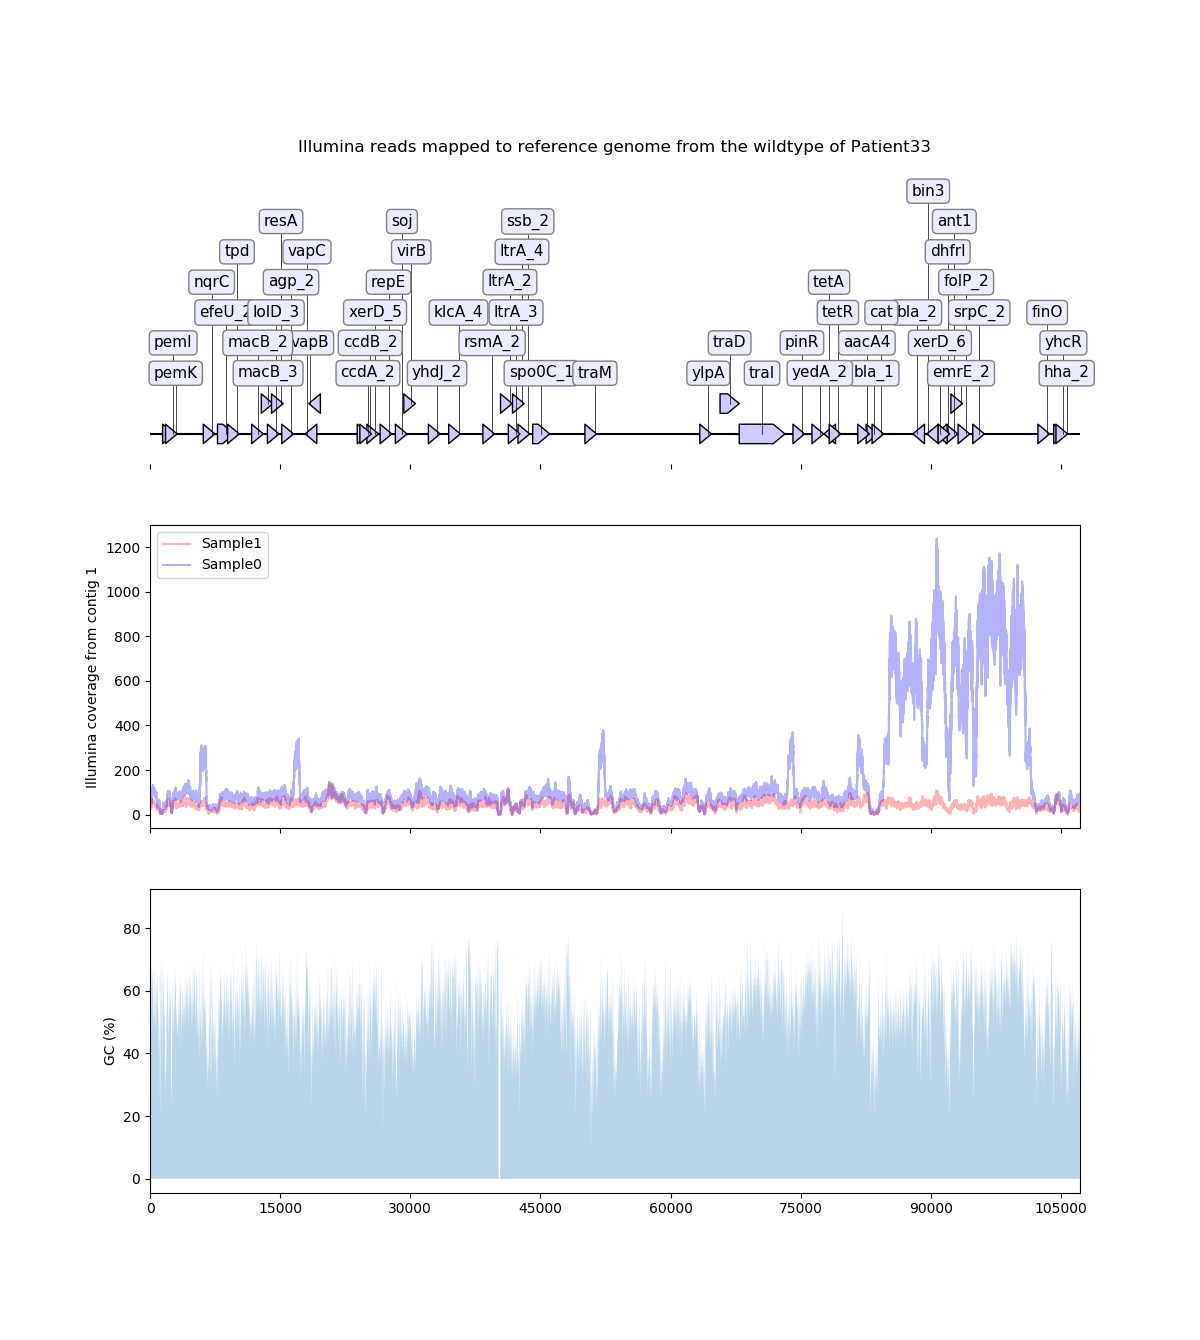
\includegraphics[scale=0.3]{coverage_pat33.png}
	\caption{Upper figure: Annotation of the whole plasmid. Middle figure: Coverage of the illumina sequencing data from sample 0 (resistant sample) and sample 1 (susceptible sample). Buttom figure: GC content.}
	\label{figure:coverage}
\end{figure}

\begin{figure}
	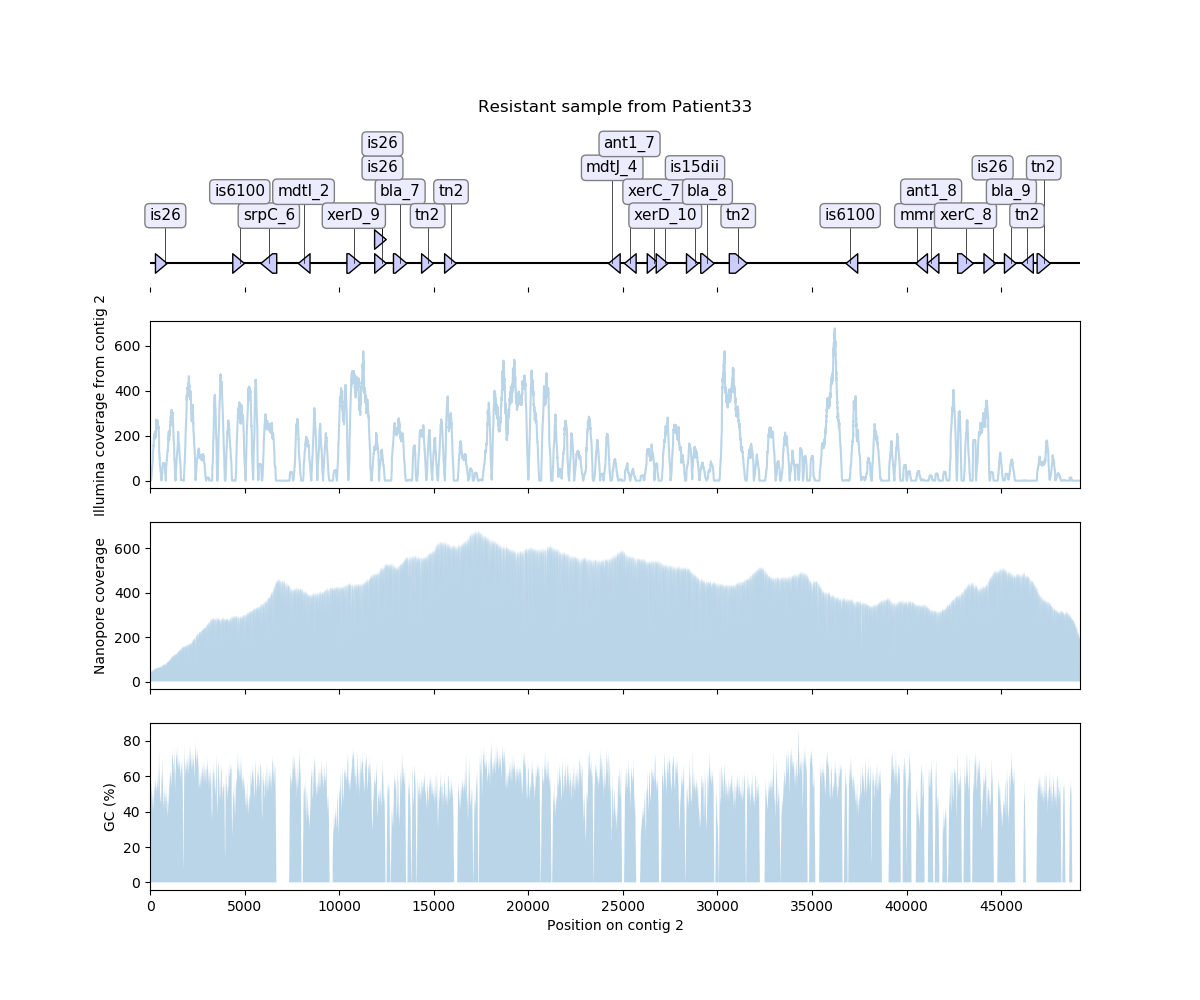
\includegraphics[width=0.5\textwidth]{sample0_plasmid.png}
	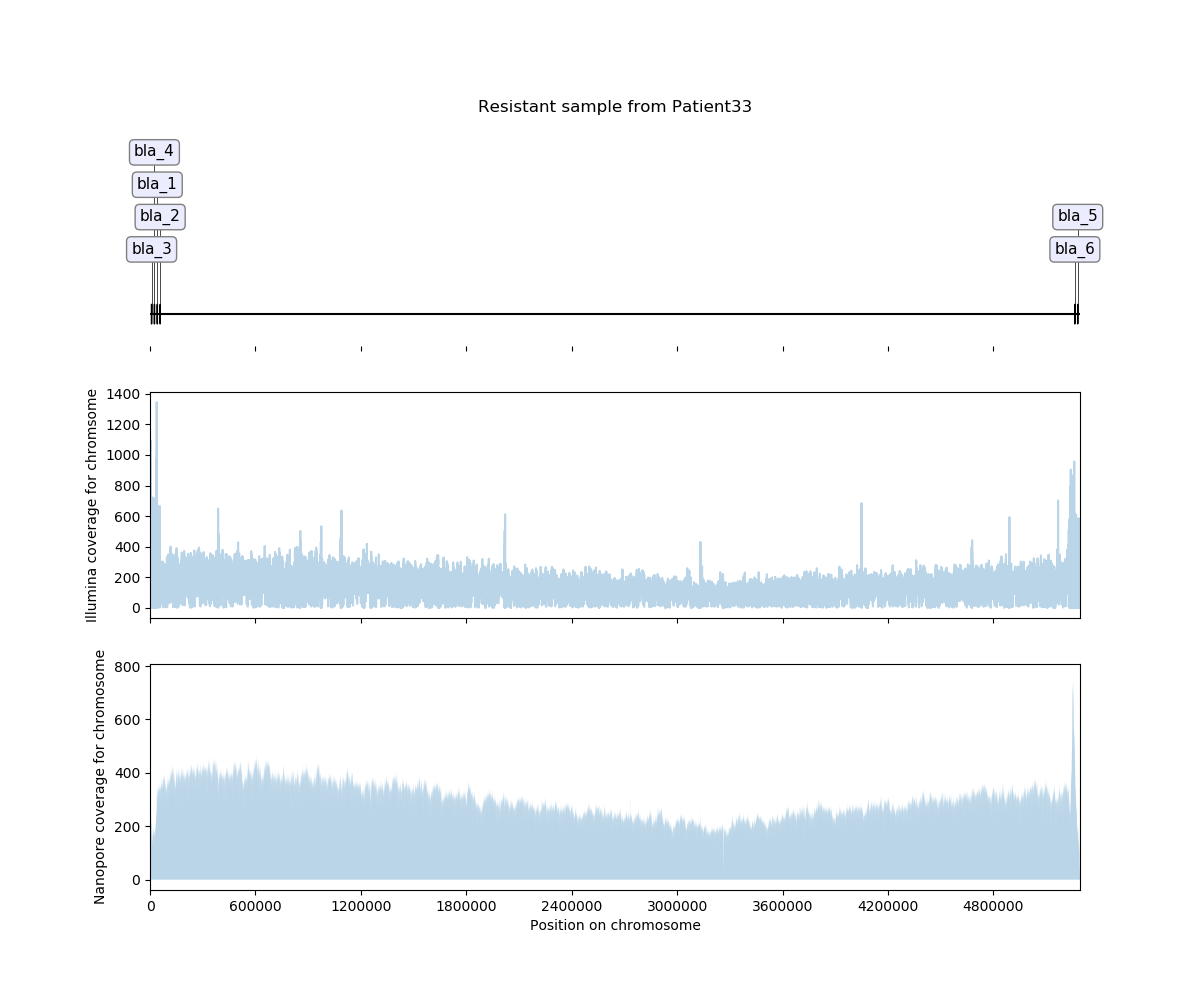
\includegraphics[width=0.5\textwidth]{sample0_chrom.png}
	\caption{}
\end{figure}
	
\subsection{Comparing ESBL genes in the resistant samples and the susceptible samples}
Since we long-read sequenced every sample from Table \ref{table:samples_overview} we hybrid-assembled and annotated those samples as well. This allowed us to see what ESBL genes were present in the susceptible and the resistant samples. The present ESBL genes and their copy numers are shown in Figure \ref{figure:esbl_genes}. Except for patient 33 there was no significant change in the copy numbers. But interestingly many strains lost or took up new ESBL genes over time. 
\begin{figure}[H]
	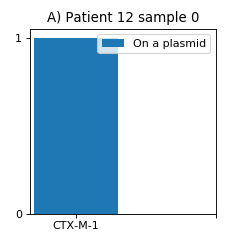
\includegraphics[width=.25\textwidth]{pat12s0.png}
	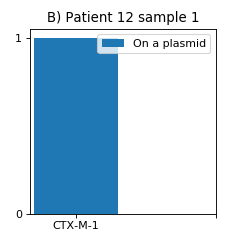
\includegraphics[width=.25\textwidth]{pat12s1.png}	
	
	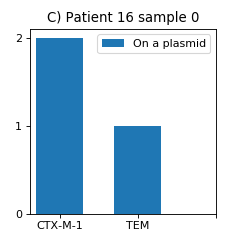
\includegraphics[width=.25\textwidth]{pat16s0.png}
	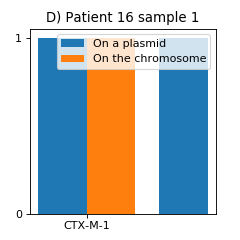
\includegraphics[width=.25\textwidth]{pat16s1.png}
	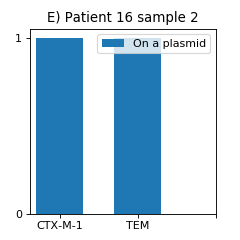
\includegraphics[width=.25\textwidth]{pat16s2.png}
	
	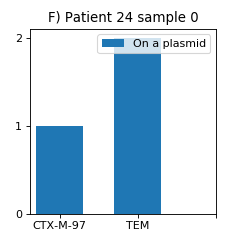
\includegraphics[width=.25\textwidth]{pat24s0.png}
	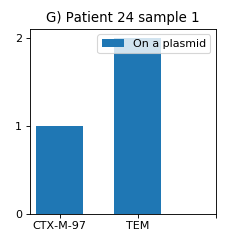
\includegraphics[width=.25\textwidth]{pat24s1.png}
	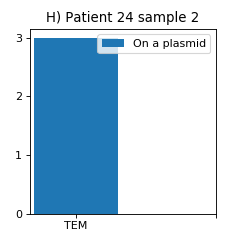
\includegraphics[width=.25\textwidth]{pat24s2.png}
	
	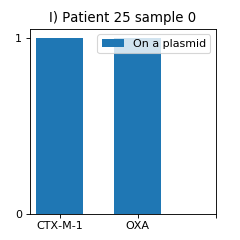
\includegraphics[width=.25\textwidth]{pat25s0.png}\hfill	
	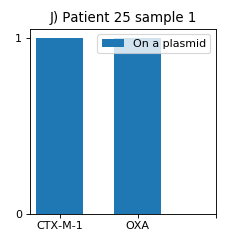
\includegraphics[width=.25\textwidth]{pat25s1.png}\hfill
	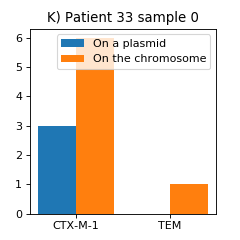
\includegraphics[width=.25\textwidth]{pat33s0.png}\hfill
	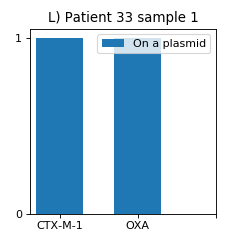
\includegraphics[width=.25\textwidth]{pat33s1.png}\hfill

	\caption{Copy numbers of ESBL genes. A-B: Patient 12, sample 1 resistant. C-E: Patient 16, sample 1 and 2 resistant. Change of copy number of CTX-M-1 and TEM. F-H: Patient 24, sample 1 resistant. CTX-M-97 was lost over time, increase of TEM copy number. I-J: Patient 25, sample 0 resistant. K-L: Patient 33 sample - resistant. Resistant sample has 8 more copies of CTX-M-1 where most of the copies are located on the chromosome.}
	\label{figure:esbl_genes}
\end{figure}

\section{Morbidostat experiments}
\subsection{Testing the continuous experiment}
The MIC of amoxicillin was determined as 2000 ng/\textmu l. The grow curve which was recorded before the initial experiment is shown in Figure \ref{figure:grow_curve}. It's visible that the growth slows down at an OD of 0.3, which is because 10 fold diluted media was used. 
\begin{figure}
	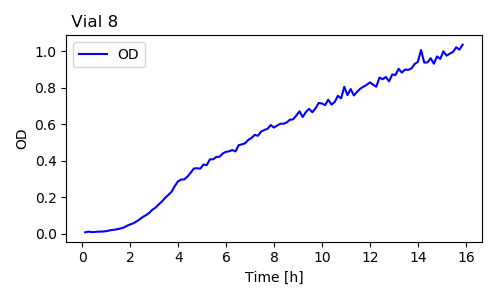
\includegraphics[width=.5\textwidth]{grow_curth.png}\hfill
	\caption{Grow curve of XL1 blue E. coli with 10 fold diluted LB media}
	\label{figure:grow_curve}
\end{figure}
The ODs and amoxicillin concentrations for the continous morbidostat experiment are shown in Figure \ref{figure:continuos_test}. Measuring of the OD for vial 1 behaved weirdly for the first 10 hours. This was caused by wrong calibration of the OD measuring unit, causing problems of detecting the right OD at low ODs. At around 40 hours 200 \textmu l of every cell susepension was transferred into 18 ml of new diluted media. It's visible that the accuracy of the OD measurement decreased before this dilution. That's because many dead cells caused scattering of the light which falsifies the OD measurement. In the second half of the experiment the drug concentrations were very high. Somehow the high amoxicillin concentration led to milky suspension when injected to the vials. This explanis why the OD measurements were more fuzzy towards the end. Also we observed that dead cells formed filament like aggregations. By stirring this sometimes caused wrong OD measurements as visible for vial 6 in Figure \ref{figure:continuos_test} at the end of the experiment. The morbidostat reacted very well to the detected growth of every vial. The target OD was set to 0.15 and every vial approximated this OD over time. Furthermore the algorithm reacted well by diluting with media when the cells died, or by increasing the drug concentration when the cells grew fast. \\
\begin{figure}
	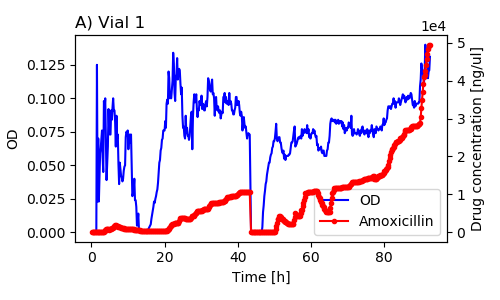
\includegraphics[width=.33\textwidth]{vial_1.png}\hfill
	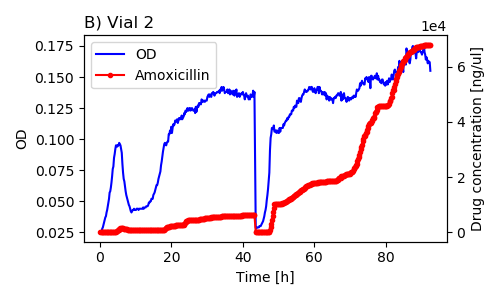
\includegraphics[width=.33\textwidth]{vial_2.png}\hfill
	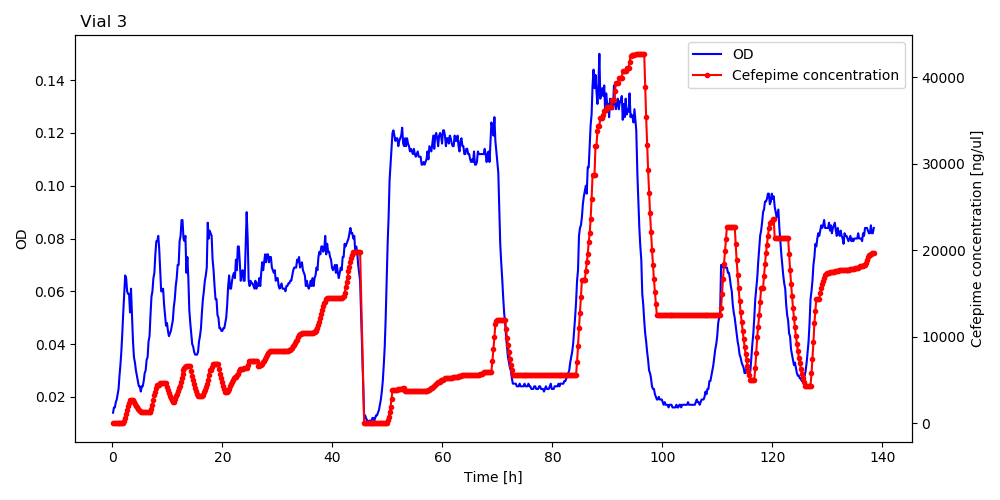
\includegraphics[width=.33\textwidth]{vial_3.png}\hfill
	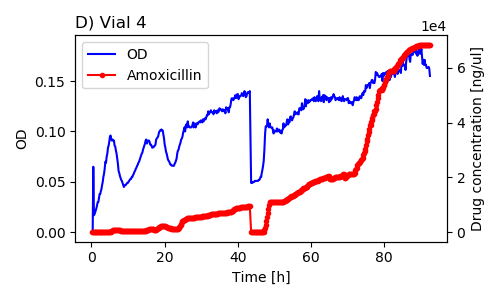
\includegraphics[width=.33\textwidth]{vial_4.png}\hfill
	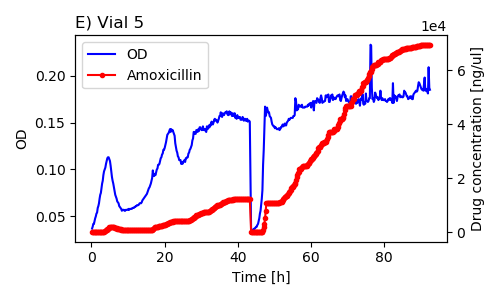
\includegraphics[width=.33\textwidth]{vial_5.png}\hfill
	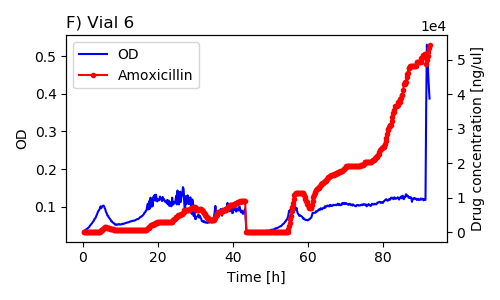
\includegraphics[width=.33\textwidth]{vial_6.png}\hfill
	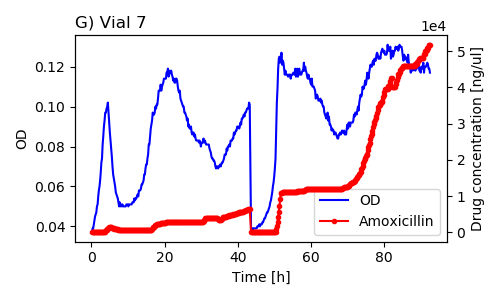
\includegraphics[width=.33\textwidth]{vial_7.png}\hfill
	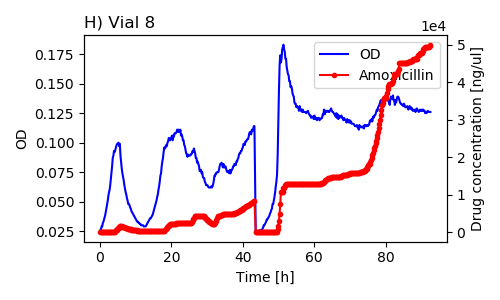
\includegraphics[width=.33\textwidth]{vial_8.png}\hfill
	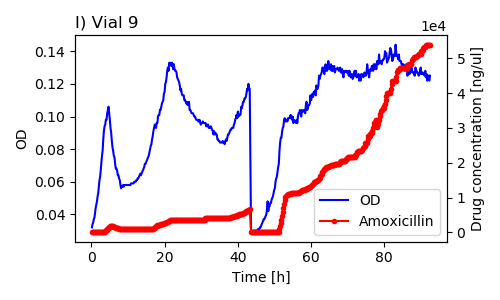
\includegraphics[width=.33\textwidth]{vial_9.png}\hfill
	\caption{For the continuous morbidstat experiment we cultured XL1 blue E. coli in 9 vials. Each plot shows the OD and the amoxicillin concentration for each vial over the whole experiment time (4.5 days). Dilution factor was 0.94, cycle time 12 minutes and the target OD 0.15. The kink in the OD and drug concentrations at 42 hours comes from transferring 200 \textmu l into new diluted media.}
	\label{figure:continuos_test}
\end{figure}
To get a better idea how the feedback reacted the first 40 hours of vial 8 are shown enlarged in Figure \ref{figure:continuos_test}. In this Figure it's visbile that no drug was injected until the OD of the vial was higher than the the drug\_dilution\_threshold (0.7). After that the amoxicillin concentration was constantly increased until the cells started to die. At the point where the OD decreased the concentration was stored which was 2000 ng \textmu /ml which is the same value as the MIC determined before the experiment. While the cells were dying media was added until the concentration was a quarter of the concentration which was necessary to kill the cells. With the cells starting to grow again, the drug concentration was increased up to the point where the cells started to die again. As visible in the Figure \ref{figure:vial8_zoom} double of the MIC was necessary to kill the cells this time.  
\begin{figure}
	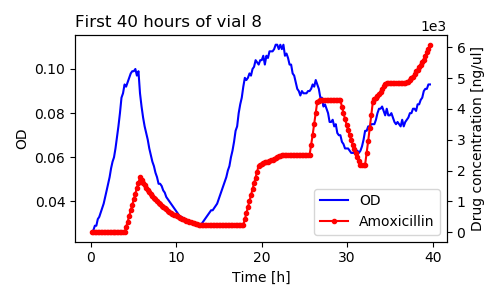
\includegraphics[width=.5\textwidth]{vial_8_zoom.png}
	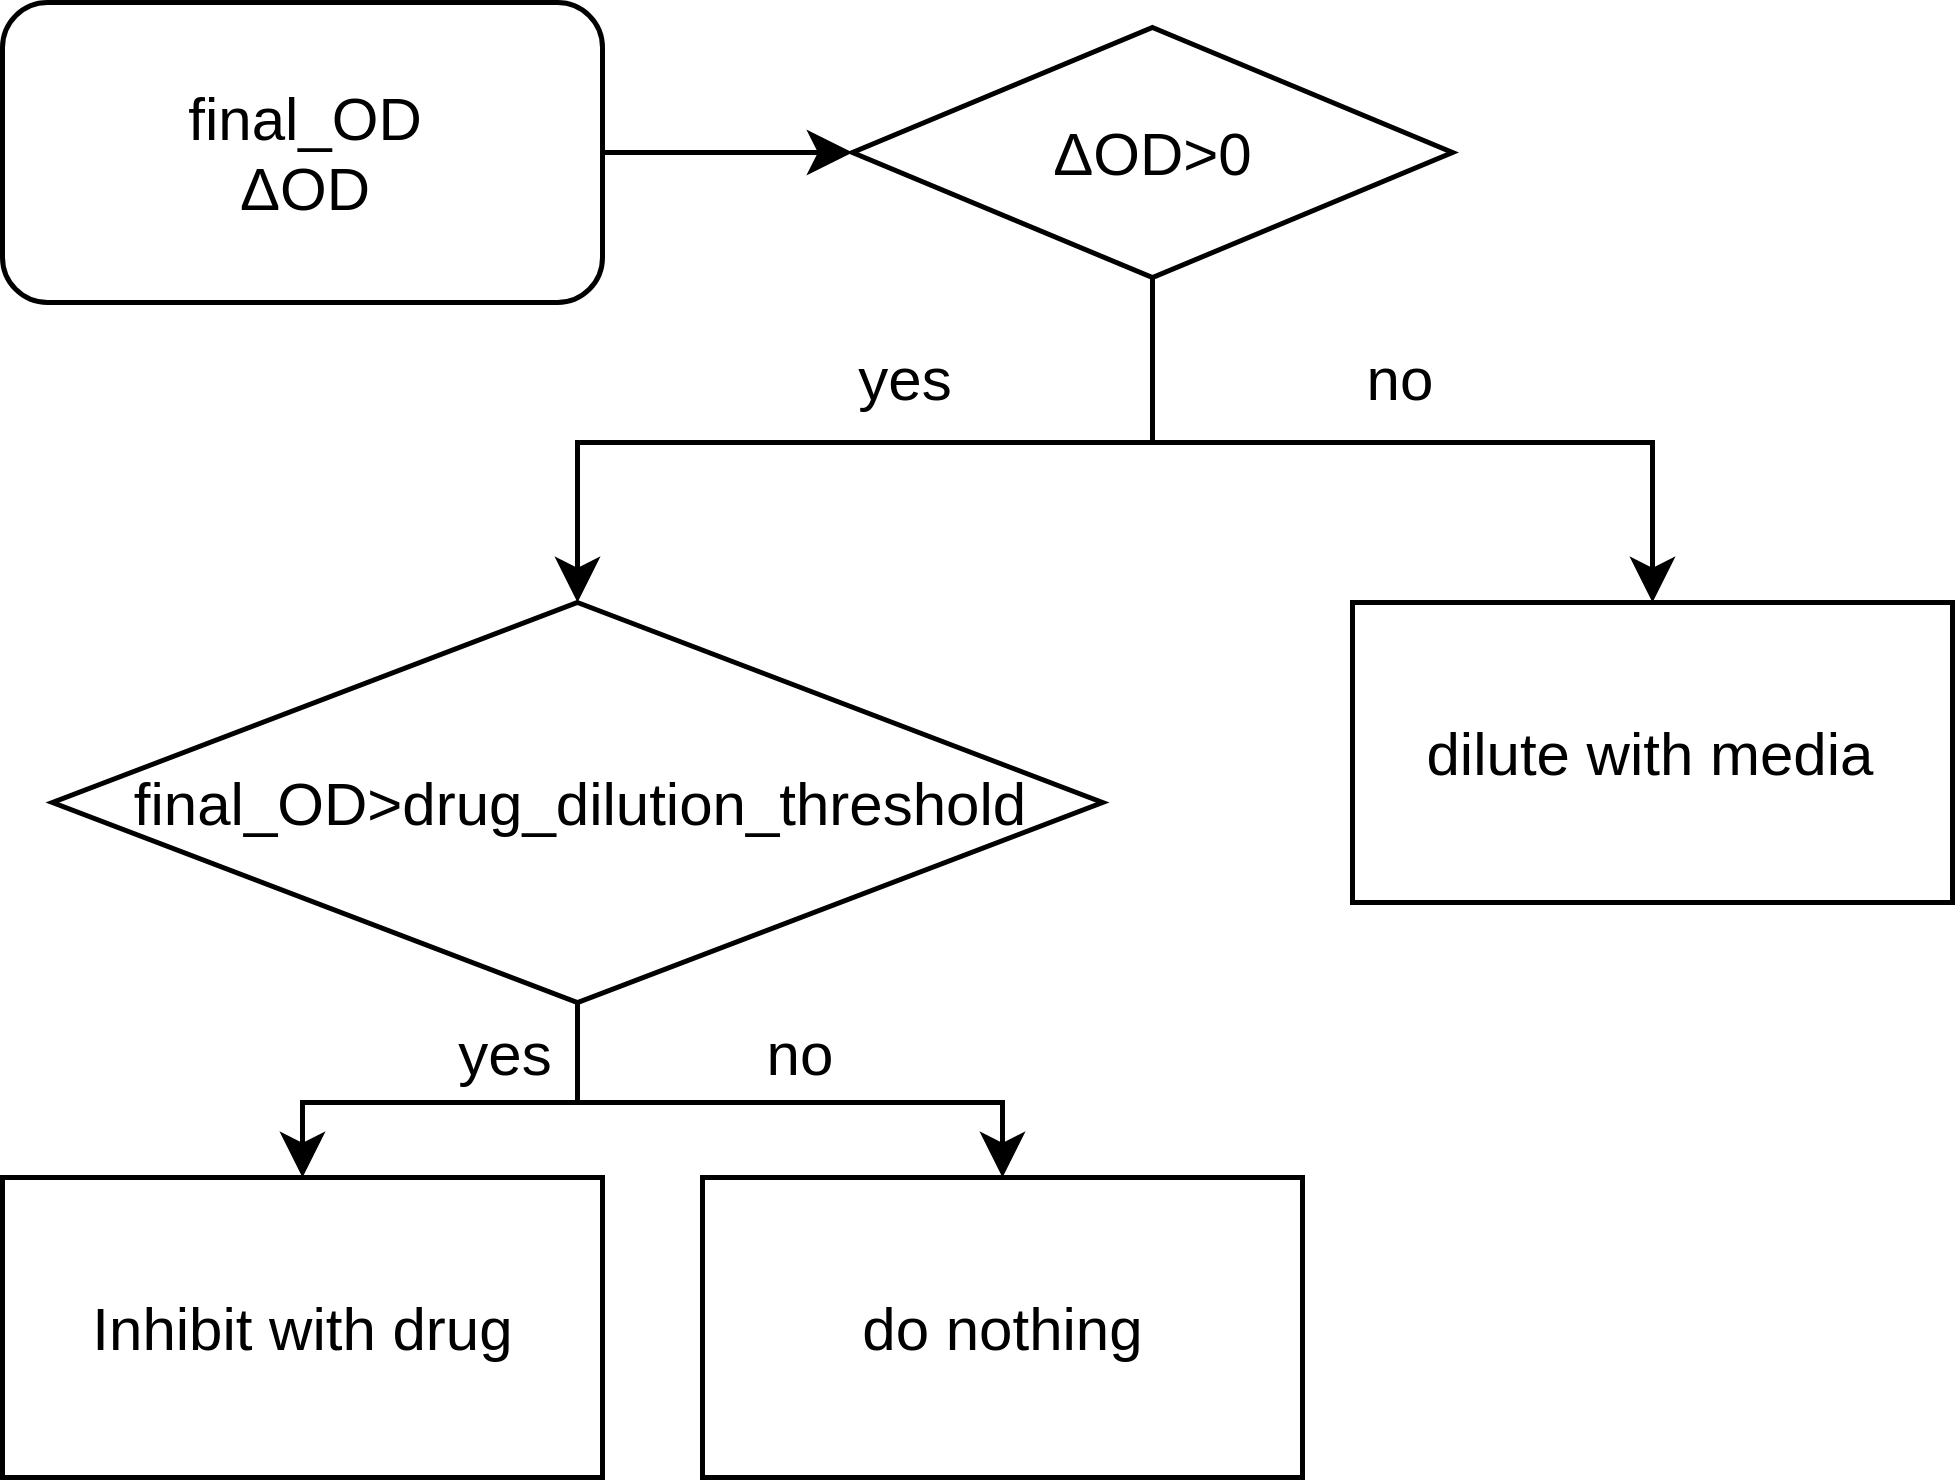
\includegraphics[width=.5\textwidth]{feedback.png}
	\caption{Left: First 40 hours of vial 8 from the continuous morbidostat. For the whole experiment time see Figure \ref{figure:continuos_test}. Right: Feedback algorithm deciding over drug injections. }
	\label{figure:vial8_zoom}
\end{figure}

\subsection{Morbidostat experiment 01}
\begin{figure}[H]
	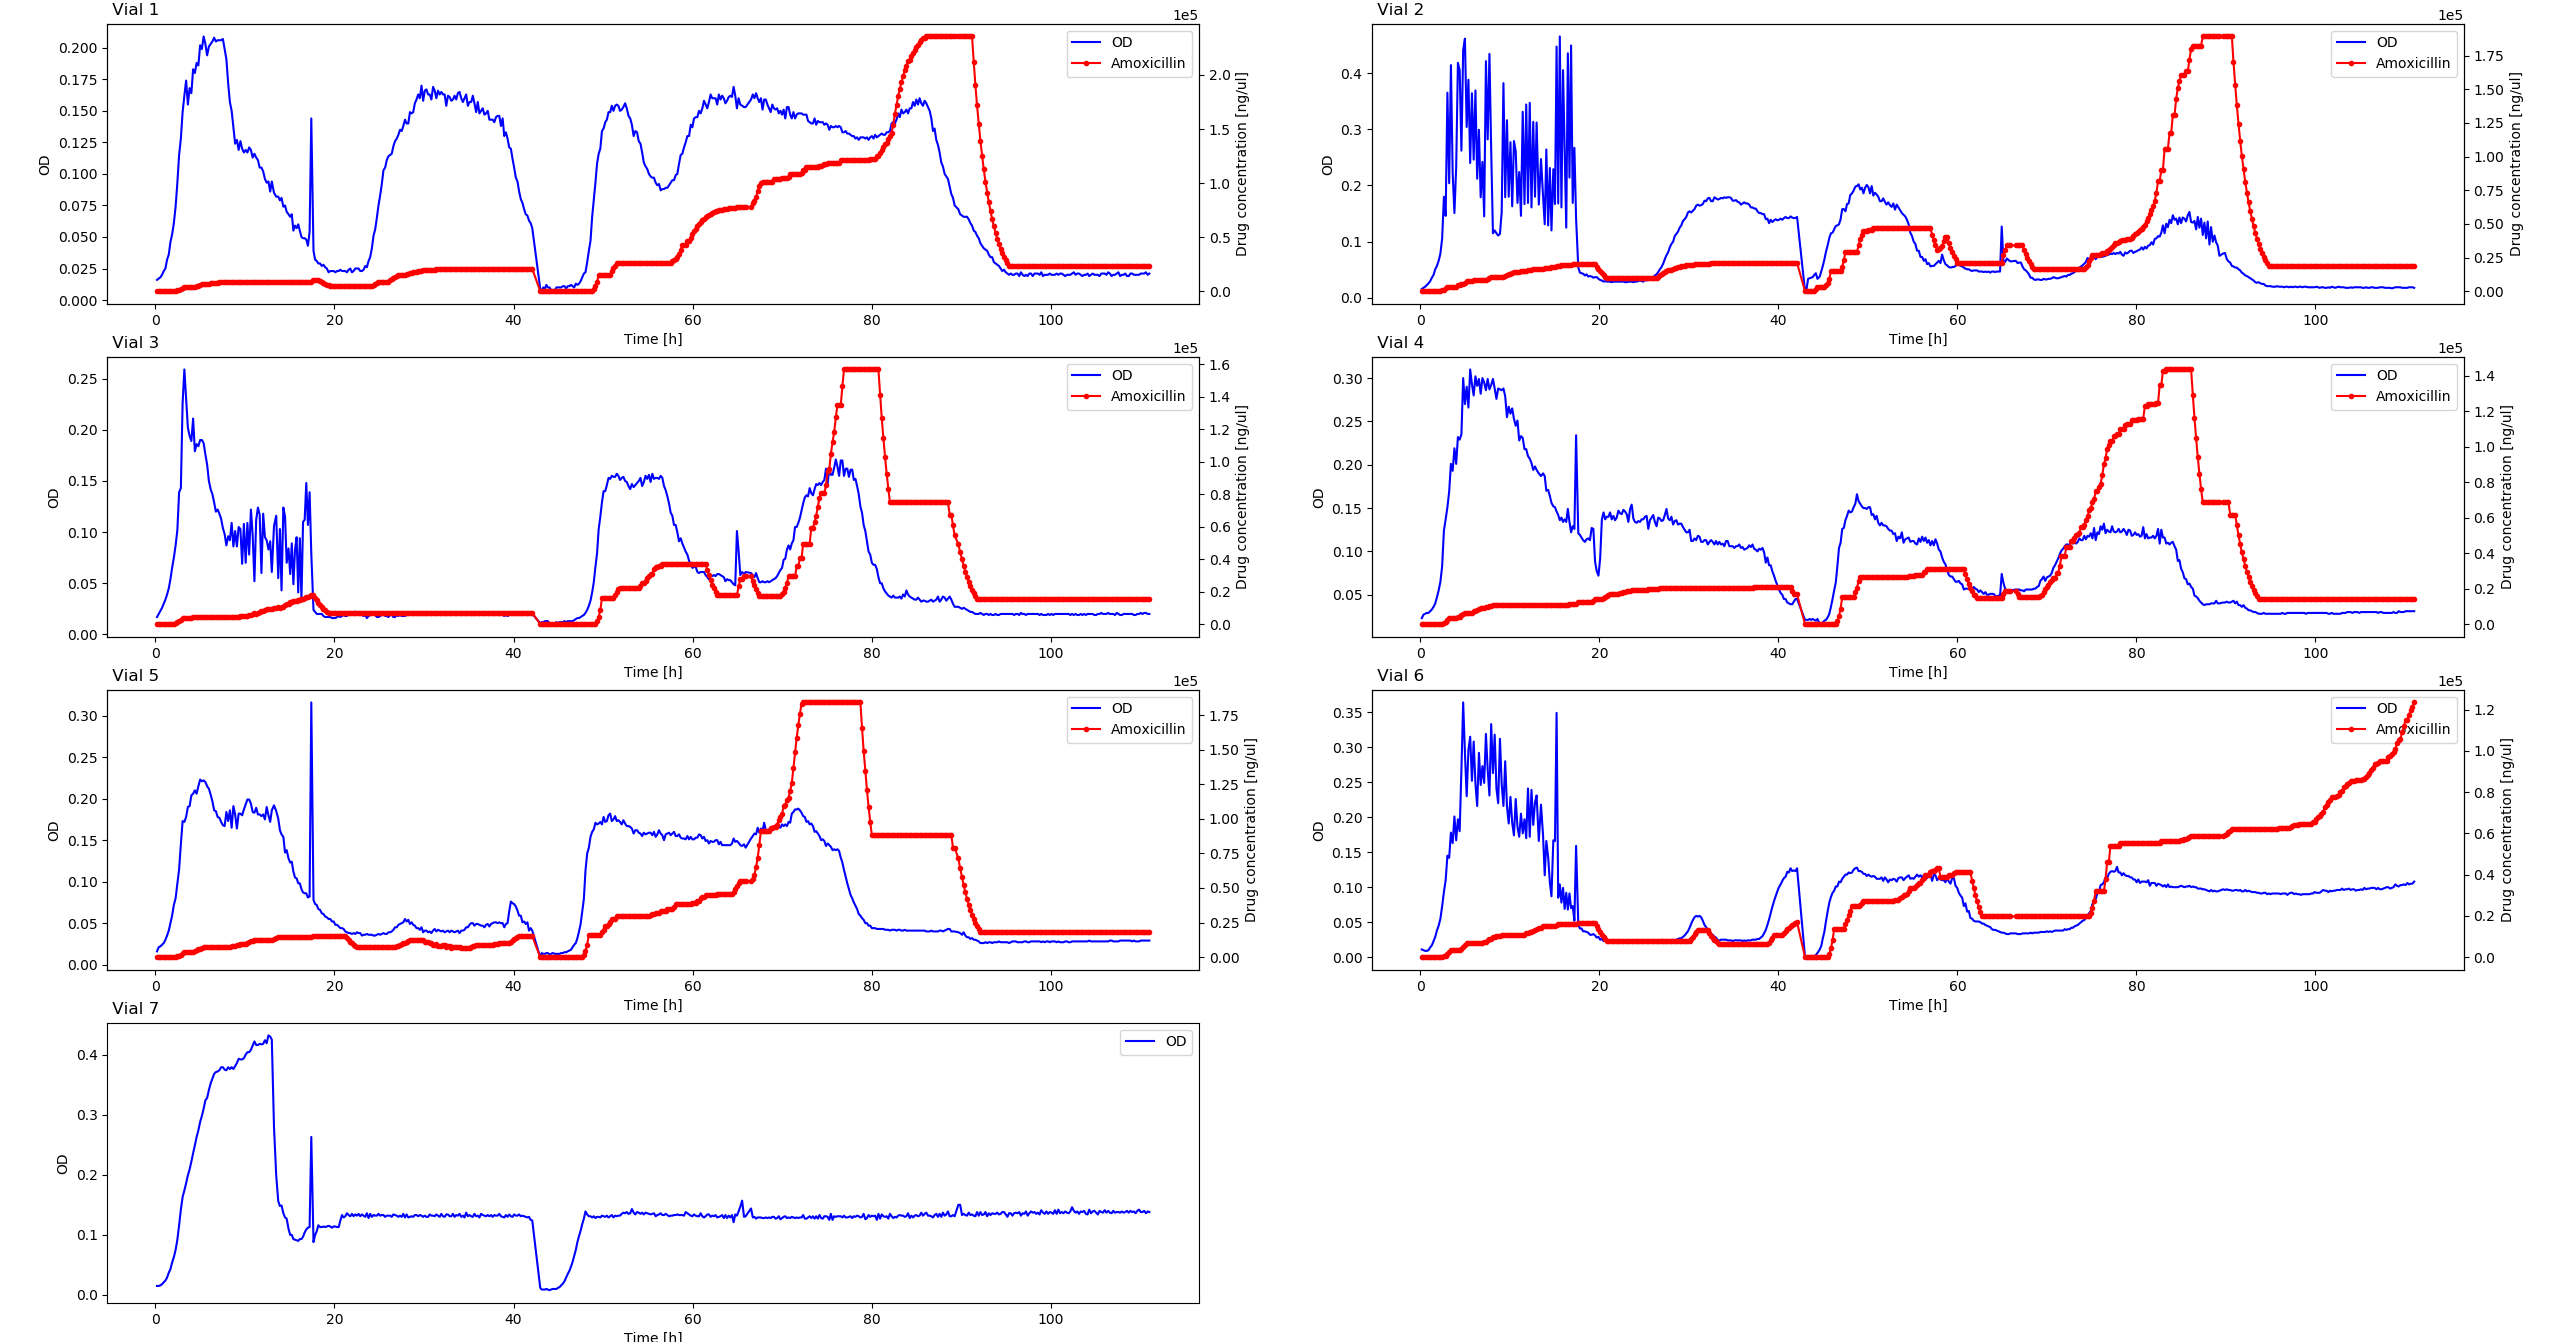
\includegraphics[width=1\textwidth]{01_morb_exp.png}
\end{figure}


\subsection{Morbidostat experiment 02}
\begin{figure}[H]
	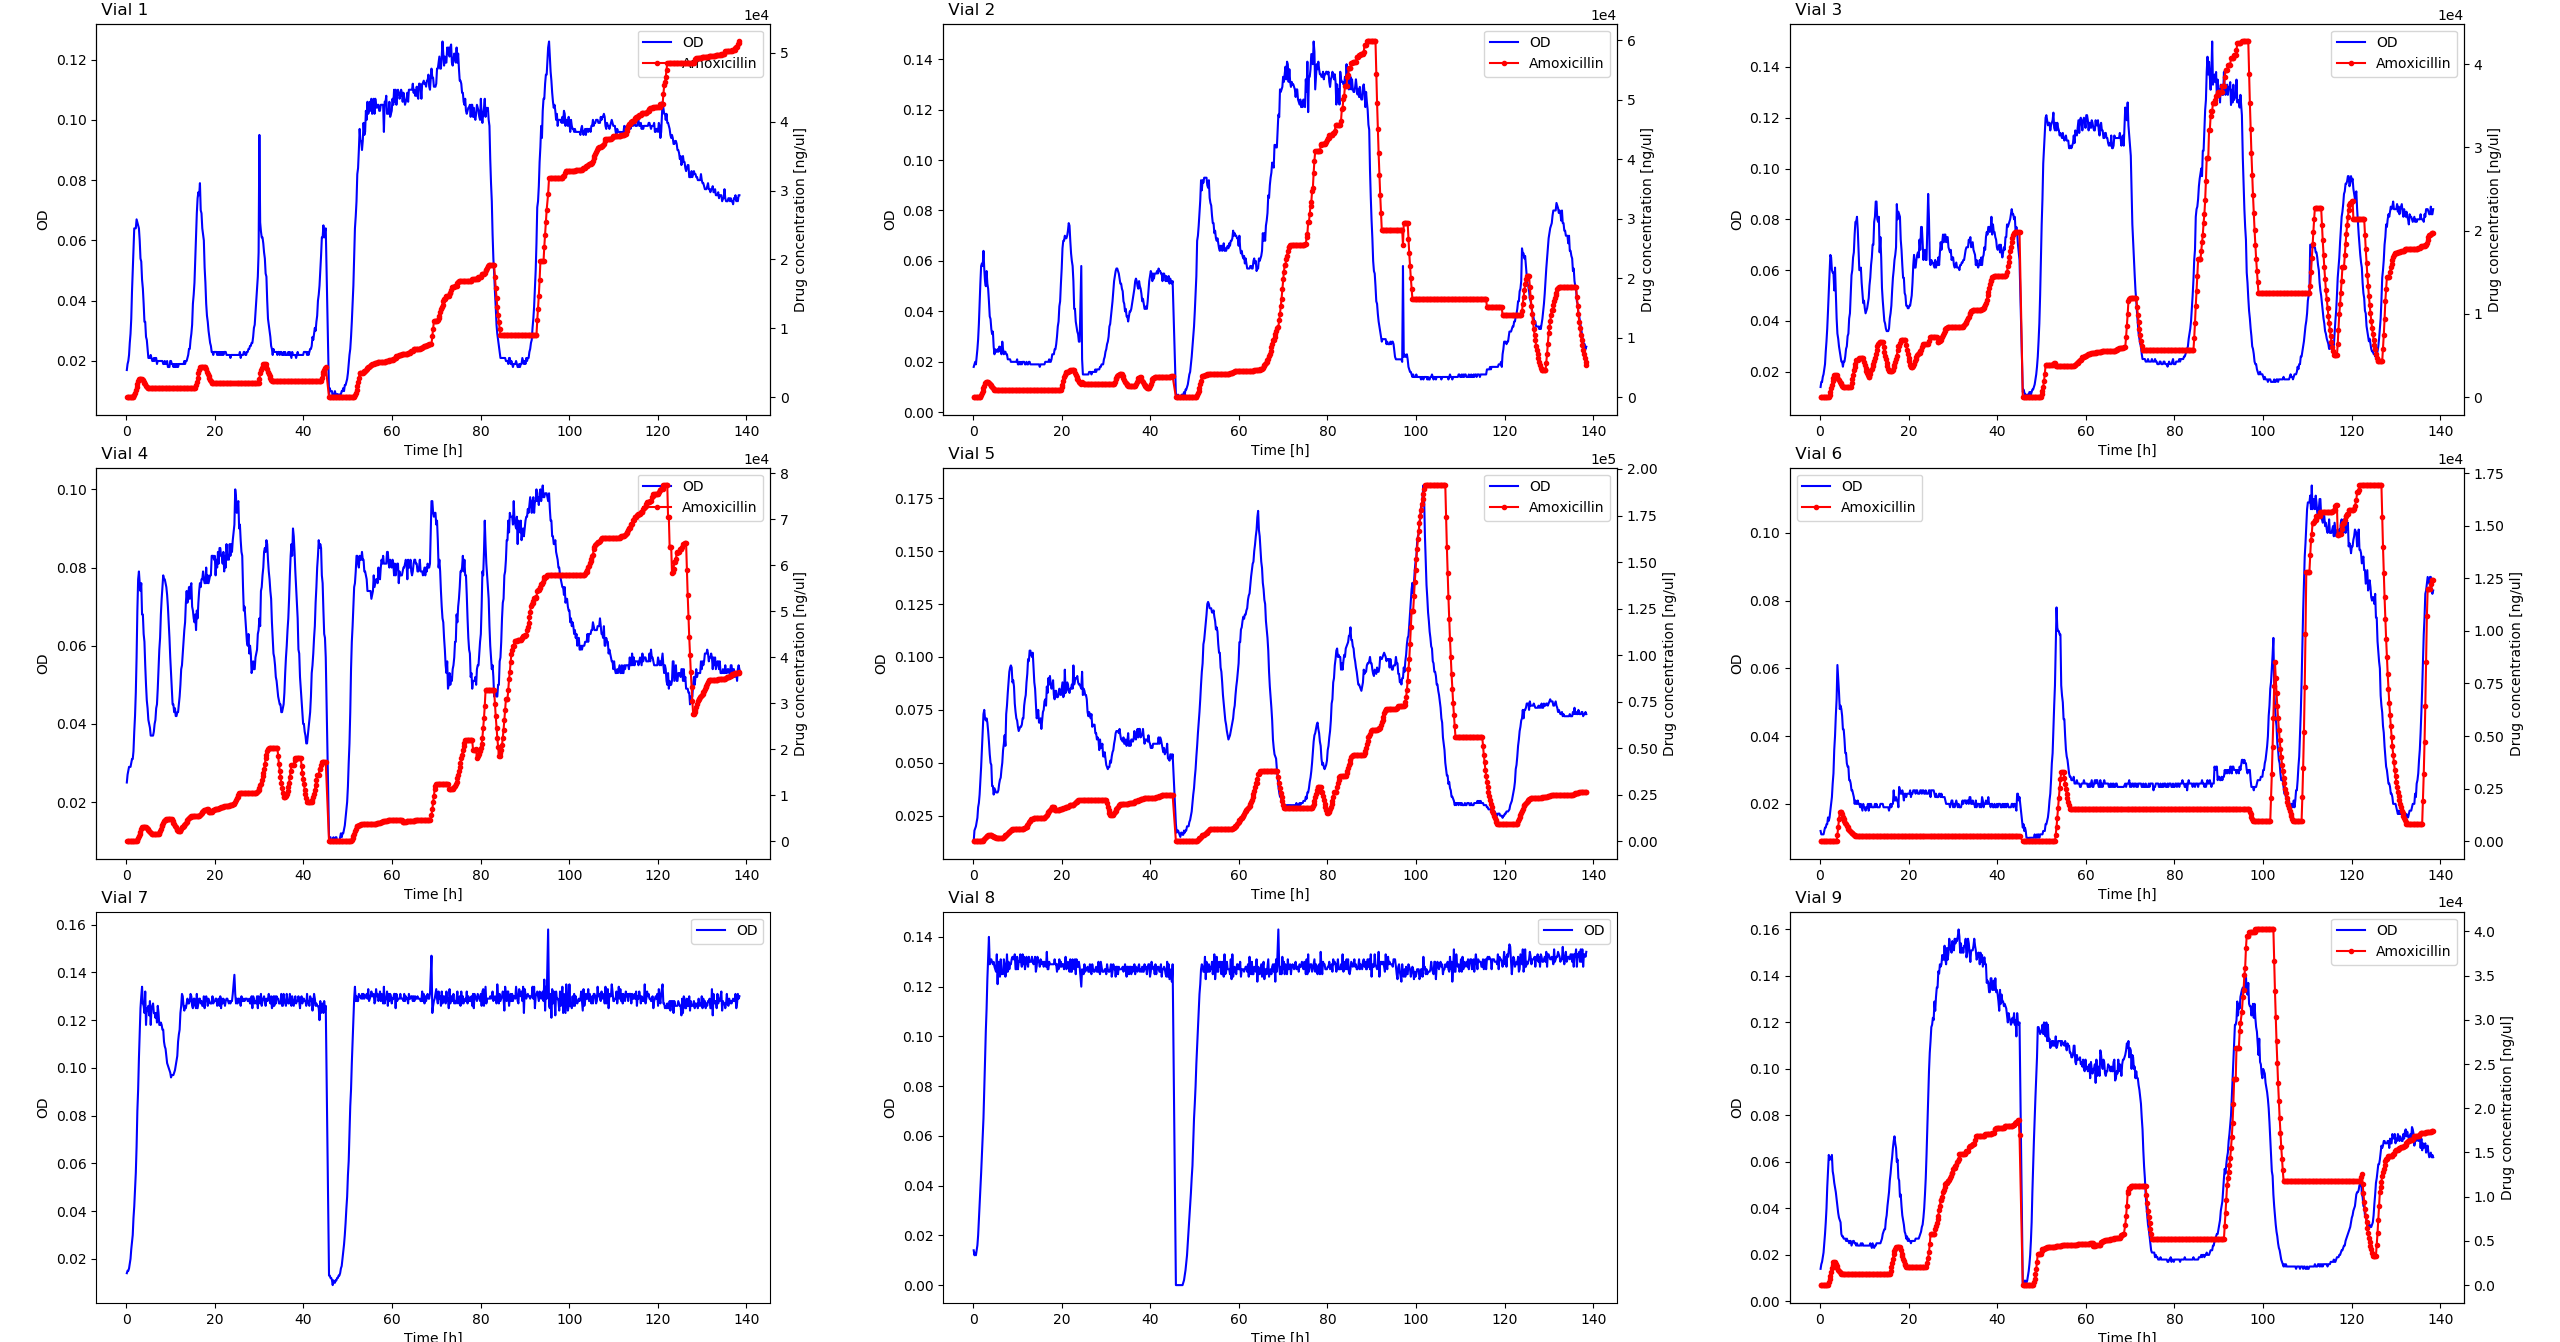
\includegraphics[width=1\textwidth]{02_morb_exp.png}
\end{figure}

\chapter{Discussion}
With this thesis I studied the evolution of cephalosporin resistance of ESBL \textit{E. coli}. I established a bioinformatic pipeline which we used to identify changes in the genome while further resistance to cephalosporines evolved in ESBL \textit{E. coli}. This pipeline was applied to next generation sequencing data coming from ESBL samples isolated from patients at the University Hospital of Basel. Furthermore, I assembled a morbiostat which we used to experimentally evolve resistance with ESBL \textit{E. coli} to cefepime. Samples taken from the morbidostat were analyzed with the established bioinformatic pipeline. 

\section{Technical and experimental challenges with the morbidostat}
\subsection{Hardware issues}
We faced problems with the computer controllable pumps that we used for injecting antibiotics and media. The controllers and the piezo pumps reacted very sensitive to small currents flowing through the digital pins of the microcontroller. This caused malfunctions of the pumps. We were able to fix this issue by connecting pull-down resistors the digital pins of the microcontroller and the ground. Furthermore, we connected inverters in serial to the digital pins which increased the reliability of the pumps. We saw in the morbidostat experiment 01, that stirring created air cones which affected th OD measurements. This is why we had to reduce the stirring to a minimum. Generally strong stirring would be beneficial because it would guarantee equal antibiotic concentrations in the vials. We could increase stirring if we would lower the OD measuring units. For controlling the morbidostat we used a 2560 Arduino mega microcontroller which has a total of 54 digital pins. In fact we used 53 digital pins which means that we were very close to the limit. If there would be the need of adding computer controllable elements to the morbidostat, another microcontroller would have to be installed. 

\subsection{Software issues}
Our microcontroller could only execute one task after another. This means that we had to ensure, that the python scripts were sending the commands one after another, instead of sending multiple commands at once. Therefore, we had to thread the command.  Even though threaded the commands we encountered a problem with the microncontroller once caused by receiving multiple commands at once. Potentially the OD measurements interfered with changing the state of the digital pins and the microcntroller crashed. All the pumps did not turn off and all the vials were overflowing. Therefore, we added a reset function which recognizes when the microcontroller crashes and automatically hard resets the microcontroller. 

\subsection{\textit{Bacillus cereus} contamination of the morbidostat experiments}
The majority of our vials were contaminated with \textit{Bacillus cereus}. Since all the stocked strains which we used for starting morbidostat experiments were not contaminated, the contamination entered the system during the experiment, or sterilization was not successful. For sterilizing we used 1 L of 3\% citric acid and 1 L of 3\% bleach. Both solutions were pumped through all the tubing over one hour. Additionally every piece of hardware, except the pumps, were autoclaved. \textit{Bacillus cereus} is a gram-positive, endospores forming bacteria \cite{bintsis_foodborne_2017}. It is possible that \textit{Bacillus cereus} endospores overcame the sterilization protocol. A study reported that after exposing \textit{Bacillus cereus} endospores with 10\% bleach for 15 minutes they were still able to produce colonies \cite{robertson_effect_2018}. Alternatively the \textit{Bacillus cereus} contamination entered the system while taking samples or exchanging the media and drug bottles. \\
Cefepime is supposed to be especially active against gram-positive bacteria because the peptidoglycan is not protected by an outer membrane \cite{sykes_chapter_2014}. Therefore, it is generally surprising, that \textit{Bacillus cereus} survived culturing with high doses of cefepime. Possibly \textit{Bacillus cereus} was able to up take the ESBL plasmid from the ESBL \textit{E. coli} strains by natural competence, which decreased the susceptibility. Alternatively \textit{Bacillus cereus} was killed by the high cefepime concentration but the high antibiotic pressure induced the formation of endospores. For sequencing we inoculated LB with kanamycin with the sample stocks and cultured them overnight. During this steps the endospores could have switched to the vegetative cycle causing the contamination in the stocks passed for sequencing.

\section{Bioinformatic challenges}
We only analyzed isolates of a patient with our bioinformatic pipeline where we ensured with phylogenetic analysis that all the samples were the same ESBL \textit{E. coli} strain. Isolates of patient 16 revealed 21 SNPs. It is unlikely that all of those SNPs are a result of resistance evolution. It is possible that the patient got reinfected with a slightly different ESBL \textit{E. coli} strain which resulted in this high number of SNPs in the isolates. Generally it was not possible to ensure that identified SNPs are related to resistance evolution. Likely many patients were treated with other drugs than antibiotics as well which could also cause evolution of the ESBL \textit{E. coli} strains. \\
The weakness of the bioinformatic pipeline was the annotation of the SNPs. For some SNPs no annotation was found by prokka \cite{seemann_prokka:_2014}, the tool we used for annotating our reference genome, but blasting of the affected sequences revealed annotation for some SNPs with no annotation.
For consistency we only presented annotation found by prokka \cite{seemann_prokka:_2014}. 

\section{Biological importance of operons targeted by mutations}
The following section describes operons targeted by SNPs in patient isolates and morbidostat samples where literature was available describing their role in the resistance to cephalosporins, or where the operons are part of a pathway possibly important for cephalosporin resistance.

\subsubsection{OrtT}
OrT is a toxin causing membrane damage resulting in reduced growth and increased persistence during stress, related to amino acid and DNA synthesis \cite{islam_orphan_2015}. Cells in the persistent state are more tolerant to antibiotics \cite{islam_orphan_2015}. Treating cells with several antibiotics such as sulfamethoxazole increased the expression of OrtT 80 fold. 

\subsection{DNA-directed RNA polymerase subunit \textbeta}
The DNA-directed RNA polymerase subunit \textbeta \space is encoded by the gene \textit{rpoB}. One paper suggests the importance  of \textit{rpoB} mutations for \textbeta-lactam resistance. Samantha Palace \textit{et al.} studied three ceftriaxone (a third-generation cephalosporin) resistant \textit{Neisseria gonorrhoeae} isolates and found one mutation affecting the \textit{rpoB} gene in all isolates \cite{palace_rna_2019}. The mutation reported by Samantha Palca \textit{et al.} was affecting a different position in the \textit{rpoB} gene than we found in the isolate of patient 16. By introducing the mutation with PCR in ceftriaxone susceptible \textit{Neisseria gonorrhoeae} strains they were able to achieve similar ceftriaxone MICs to the resistant isolates, indicating the importance of the mutated \textit{rpoB} gene for the resistance mechanism \cite{palace_rna_2019}. It is not understood yet, how the mutated \textit{rpoB} leads to ceftriaxone resistance. \\


\subsubsection{RNA polymerase sigma factor RpoD}
RpoD is a sigma factor which targets RNA polymerase to a wide range of promoters \cite{maciag_vitro_2011}. The same paper which found mutated \textit{rpoB} genes in ceftriaxone resistant \textit{Neisseria gonorrhoeae} isolates, also found mutated \textit{rpoD} genes in some isolates. The mutation that we found affects a different postion than the one found by Samantha Palace \textit{et al.}. They were able to reproduce resistance by mutating the \textit{rpoD} gene of a ceftriaxone suscecptilbe \textit{Neisseria gonorrhoeae} strain. Similar to mutations in the \textit{rpoB} gene, it is not understood yet, how mutations in the \textit{rpoD} gene can lead to resistance.  

\subsection{FepA promoter}
One mutations was found in the promoter regulating the expression of the protein FepA. FepA is a gated outer membrane porin transporting unspecific hydrophilic substances \cite{liu_permeability_1993}. Potentially the mutation in the promoter of FepA reduced the expression which potentially reduces the uptake of cephalosporins.  

\subsection{Transcriptional regulatory protein OmpR}
OmpR is a DNA-binding protein that interacts with the upstream promoter region of the \textit{ompF} and \textit{ompC} genes and regulates their expression \cite{rampersaud_ompr_1994}. OmpC and OmpF are the two major outer membrane proteins in \textit{E. coli} and have been reported for playing an important role in \textbeta-lactam resistance \cite{rampersaud_ompr_1994} \cite{fernandez_adaptive_2012}.

\subsubsection{Osmolarity sensor protein EnvZ}
As OmpR, EnvZ is involved in regulating the expressions of OmpC and OmpF \cite{rampersaud_ompr_1994}. EnvZ is a transmembrane sensor which detects the osmotic pressure and phosporolates OmpR depending on the detected osmolarity \cite{rampersaud_ompr_1994}. At low osmolarity, EnvZ modulates low levels of phosphorylated OmpR, at high osmolarity OmpR mediates high levels of phosphorylated OmpR \cite{rampersaud_ompr_1994}. Phosphorylated OmpR increases the expression of \textit{ompC} gene while repressing the expression of \textit{ompF} gene \cite{rampersaud_ompr_1994}. If OmpR is not phosphorylated, expression of the gene \textit{ompF} is increased and \textit{ompC} repressed. Becerio A \textit{et. al} reported that two cefepime resistant ESBL \textit{E. coli} isolates lack the OmpC and OmpF porins \cite{beceiro_false_2011}. A lack of those porins likely heavily reduces the cefepime uptake.   

\subsection{Outer membrane protein F OmpF}
Cephalosporin transport occurs partly through the outer membrane protein F \cite{masi_structure_2013}. A mutation in the \textit{ompF} gene could affect the porin structure which potentially affects the cephalosporin transport. 

\subsubsection{\textbeta-lactamase CTX-M-1}
One mutation affected the gene coding for the beta-lactamse CTX-M-1. The resulting variant is not known in the literature so it is not possible to conclude whether its activity is increased or not. 
 

\subsection{Potential resistance mechanism considering mutated operons}
Considering genes targeted by SNPs in patient isolates and morbidostat samples suggests that OmpC and OmpF and their regulatory system are affecting cefepime susceptibility. Both, Ompc and OmpF are highly expressed and important for cefepime transport \cite{rampersaud_ompr_1994} \cite{masi_structure_2013}. Both are regulated by the regulatory protein OmpR. Interestingly a mutated version of OmpR was found in the isolates of patient 16 and in a morbidostat sample. The mutations in the \textit{ompR} gene were not identical, in the patient isolate a missense mutaion was present, in the morbidostat sample a nonsense mutation. OmpR binds to the operons of \textit{ompC} and \textit{ompF} which is necessary for their expression \cite{masi_structure_2013}. If OmpR is mutated it can possibly not bind to the operons and expression would be highly repressed. This makes sense in particular for the OmpR with the nonsense mutation in the morbidostat sample. The DNA binding activity of OmpR itself is regulated by EnvZ \cite{masi_structure_2013}. EnvZ is a kinase phosphorylating OmpR depending on osmotic pressure. The gene coding for EnvZ was also targeted by a SNP in a morbidostat sample. Possibly this changes the expression level of OmpC and OmpF as well. \\
The SNP altering the \textit{rpoB} could also affect cefepime susceptibility because it was proven to affect ceftriaxone susceptibility. However, it is not understood how a mutation in a RNA polymerase could affect the cephalosporin susceptibility. Interestingly one SNP in the morbidostat samples affected the RNA polymerase sigma factor RpoD. This increases the suspicion that some processes in the transcription affects the cefepime susceptibility, in a way which is not understood yet. \\
In general it seems like resistance to cefepime can be acquired by different pathways. The outer membrane proteins definitely seem to play an important role, as well as RpoD and RpoB. Other options are mutated CTX-M-1 \textbeta-lactamases which we have seen in one sample of the morbidostat, or increased persistance resulting in reduced growth. 

\chapter{References}
\phantomsection
\let\Origclearpage\clearpage
\let\clearpage\relax
\defbibheading{bibliography}[\refname]{}
\printbibliography
\newpage
\chapter{Supplementary}
\section{Manual for starting experiments with morbidostat}
\label{section:manual}





\section{SNPs with no annotation}
\label{section:snps_with_no_annotation}
\begin{longtable}{|l|l|l|l|l|}
	\cline{1-4}
	\multicolumn{1}{|l}{Patient12} & \multicolumn{1}{l}{} & \multicolumn{1}{l}{}        &                      & \multicolumn{1}{l}{}  \\ 
	\cline{1-4}
	Contig                         & Position             & \multicolumn{1}{l}{Samples} &                      & \multicolumn{1}{l}{}  \\ 
	\cline{1-4}
	0                              & 880249               & Sample0: C                  & Sample1: A           & \multicolumn{1}{l}{}  \\ 
	\cline{1-4}
	0                              & 1619787              & Sample0: G                  & Sample1: A           & \multicolumn{1}{l}{}  \\ 
	\cline{1-4}
	0                              & 2481354              & Sample0: A                  & Sample1: G           & \multicolumn{1}{l}{}  \\ 
	\cline{1-4}
	0                              & 4256761              & Sample0: A                  & Sample1: T           & \multicolumn{1}{l}{}  \\ 
	\cline{1-4}
	\multicolumn{1}{l}{}           & \multicolumn{1}{l}{} & \multicolumn{1}{l}{}        & \multicolumn{1}{l}{} & \multicolumn{1}{l}{}  \\ 
	\hline
	\multicolumn{1}{|l}{Patient16} & \multicolumn{1}{l}{} & \multicolumn{1}{l}{}        & \multicolumn{1}{l}{} &                       \\ 
	\hline
	Contig                         & Position             & \multicolumn{1}{l}{Samples} & \multicolumn{1}{l}{} &                       \\ 
	\hline
	0                              & 55597                & Sample0: A                  & Sample1: G           & Sample2: G            \\ 
	\hline
	0                              & 387261               & Sample0: C                  & Sample1: A           & Sample2: C            \\ 
	\hline
	0                              & 387282               & Sample0: A                  & Sample1: C           & Sample2: C            \\ 
	\hline
	0                              & 420182               & Sample0: T                  & Sample1: C           & Sample2: T            \\ 
	\hline
	0                              & 420183               & Sample0: G                  & Sample1: A           & Sample2: G            \\ 
	\hline
	0                              & 539392               & Sample0: G                  & Sample1: A           & Sample2: A            \\ 
	\hline
	0                              & 808891               & Sample0: C                  & Sample1: T           & Sample2: T            \\ 
	\hline
	0                              & 813579               & Sample0: T                  & Sample1: A           & Sample2: T            \\ 
	\hline
	0                              & 813613               & Sample0: C                  & Sample1: A           & Sample2: C            \\ 
	\hline
	0                              & 813614               & Sample0: C                  & Sample1: A           & Sample2: C            \\ 
	\hline
	0                              & 893946               & Sample0: C                  & Sample1: A           & Sample2: C            \\ 
	\hline
	0                              & 922702               & Sample0: G                  & Sample1: A           & Sample2: G            \\ 
	\hline
	0                              & 1133762              & Sample0: C                  & Sample1: T           & Sample2: T            \\ 
	\hline
	0                              & 1508583              & Sample0: A                  & Sample1: T           & Sample2: T            \\ 
	\hline
	0                              & 1508592              & Sample0: A                  & Sample1: T           & Sample2: T            \\ 
	\hline
	0                              & 1508611              & Sample0: -                  & Sample1: T           & Sample2: T            \\ 
	\hline
	0                              & 1508618              & Sample0: A                  & Sample1: T           & Sample2: T            \\ 
	\hline
	0                              & 1508625              & Sample0: A                  & Sample1: C           & Sample2: C            \\ 
	\hline
	0                              & 1525597              & Sample0: A                  & Sample1: G           & Sample2: A            \\ 
	\hline
	0                              & 1549518              & Sample0: T                  & Sample1: G           & Sample2: G            \\ 
	\hline
	0                              & 1729351              & Sample0: A                  & Sample1: C           & Sample2: C            \\ 
	\hline
	0                              & 2016331              & Sample0: A                  & Sample1: C           & Sample2: A            \\ 
	\hline
	0                              & 2023731              & Sample0: A                  & Sample1: T           & Sample2: A            \\ 
	\hline
	0                              & 2101129              & Sample0: C                  & Sample1: -           & Sample2: -            \\ 
	\hline
	0                              & 2101130              & Sample0: A                  & Sample1: -           & Sample2: -            \\ 
	\hline
	0                              & 2128255              & Sample0: T                  & Sample1: -           & Sample2: T            \\ 
	\hline
	0                              & 2531373              & Sample0: -                  & Sample1: T           & Sample2: T            \\ 
	\hline
	0                              & 2647199              & Sample0: T                  & Sample1: C           & Sample2: T            \\ 
	\hline
	0                              & 2798262              & Sample0: T                  & Sample1: C           & Sample2: T            \\ 
	\hline
	0                              & 2798288              & Sample0: T                  & Sample1: C           & Sample2: T            \\ 
	\hline
	0                              & 2798294              & Sample0: T                  & Sample1: A           & Sample2: T            \\ 
	\hline
	0                              & 2798312              & Sample0: A                  & Sample1: C           & Sample2: C            \\ 
	\hline
	0                              & 3503181              & Sample0: A                  & Sample1: T           & Sample2: T            \\ 
	\hline
	0                              & 3920934              & Sample0: A                  & Sample1: G           & Sample2: A            \\ 
	\hline
	0                              & 4459680              & Sample0: C                  & Sample1: -           & Sample2: C            \\ 
	\hline
	0                              & 4459681              & Sample0: C                  & Sample1: -           & Sample2: C            \\ 
	\hline
	0                              & 4459684              & Sample0: G                  & Sample1: -           & Sample2: G            \\ 
	\hline
	0                              & 4459685              & Sample0: A                  & Sample1: -           & Sample2: A            \\ 
	\hline
	0                              & 4459686              & Sample0: A                  & Sample1: -           & Sample2: A            \\ 
	\hline
	0                              & 4459687              & Sample0: G                  & Sample1: -           & Sample2: G            \\ 
	\hline
	0                              & 4459688              & Sample0: A                  & Sample1: -           & Sample2: A            \\ 
	\hline
	0                              & 4459689              & Sample0: G                  & Sample1: -           & Sample2: G            \\ 
	\hline
	0                              & 4459692              & Sample0: A                  & Sample1: -           & Sample2: A            \\ 
	\hline
	0                              & 4459693              & Sample0: G                  & Sample1: -           & Sample2: G            \\ 
	\hline
	0                              & 4459695              & Sample0: G                  & Sample1: -           & Sample2: G            \\ 
	\hline
	0                              & 4459697              & Sample0: T                  & Sample1: -           & Sample2: T            \\ 
	\hline
	0                              & 4842004              & Sample0: C                  & Sample1: T           & Sample2: T            \\ 
	\hline
	\multicolumn{1}{l}{}           & \multicolumn{1}{l}{} & \multicolumn{1}{l}{}        & \multicolumn{1}{l}{} & \multicolumn{1}{l}{}  \\ 
	\hline
	\multicolumn{1}{|l}{Patient24} & \multicolumn{1}{l}{} & \multicolumn{1}{l}{}        & \multicolumn{1}{l}{} &                       \\ 
	\hline
	Contig                         & Position             & \multicolumn{1}{l}{Samples} & \multicolumn{1}{l}{} &                       \\ 
	\hline
	0                              & 418566               & Sample0: T                  & Sample1: C           & Sample2: T            \\ 
	\hline
	0                              & 418588               & Sample0: G                  & Sample1: A           & Sample2: G            \\ 
	\hline
	0                              & 1505822              & Sample0: C                  & Sample1: A           & Sample2: A            \\ 
	\hline
	0                              & 1505825              & Sample0: A                  & Sample1: T           & Sample2: T            \\ 
	\hline
	0                              & 1925913              & Sample0: A                  & Sample1: C           & Sample2: C            \\ 
	\hline
	0                              & 1925915              & Sample0: A                  & Sample1: T           & Sample2: T            \\ 
	\hline
	0                              & 2925037              & Sample0: C                  & Sample1: T           & Sample2: T            \\ 
	\hline
	0                              & 2954867              & Sample0: C                  & Sample1: T           & Sample2: T            \\ 
	\hline
	\multicolumn{1}{l}{}           & \multicolumn{1}{l}{} & \multicolumn{1}{l}{}        & \multicolumn{1}{l}{} & \multicolumn{1}{l}{}  \\ 
	\cline{1-4}
	\multicolumn{1}{|l}{Patient25} & \multicolumn{1}{l}{} & \multicolumn{1}{l}{}        &                      & \multicolumn{1}{l}{}  \\ 
	\cline{1-4}
	Contig                         & Position             & \multicolumn{1}{l}{Samples} &                      & \multicolumn{1}{l}{}  \\ 
	\cline{1-4}
	0                              & 1998615              & Sample0: T                  & Sample1: A           & \multicolumn{1}{l}{}  \\ 
	\cline{1-4}
	0                              & 3480363              & Sample0: T                  & Sample1: C           & \multicolumn{1}{l}{}  \\ 
	\cline{1-4}
	0                              & 3743644              & Sample0: A                  & Sample1: G           & \multicolumn{1}{l}{}  \\ 
	\cline{1-4}
	0                              & 4785433              & Sample0: G                  & Sample1: A           & \multicolumn{1}{l}{}  \\ 
	\cline{1-4}
	0                              & 4785439              & Sample0: G                  & Sample1: A           & \multicolumn{1}{l}{}  \\ 
	\cline{1-4}
	\multicolumn{1}{l}{}           & \multicolumn{1}{l}{} & \multicolumn{1}{l}{}        & \multicolumn{1}{l}{} & \multicolumn{1}{l}{}  \\ 
	\cline{1-4}
	\multicolumn{1}{|l}{Patient33} & \multicolumn{1}{l}{} & \multicolumn{1}{l}{}        &                      & \multicolumn{1}{l}{}  \\ 
	\cline{1-4}
	Contig                         & Position             & \multicolumn{1}{l}{Samples} &                      & \multicolumn{1}{l}{}  \\ 
	\cline{1-4}
	0                              & 2887411              & Sample0: A                  & Sample1: C           & \multicolumn{1}{l}{}  \\
	\cline{1-4}
\end{longtable}
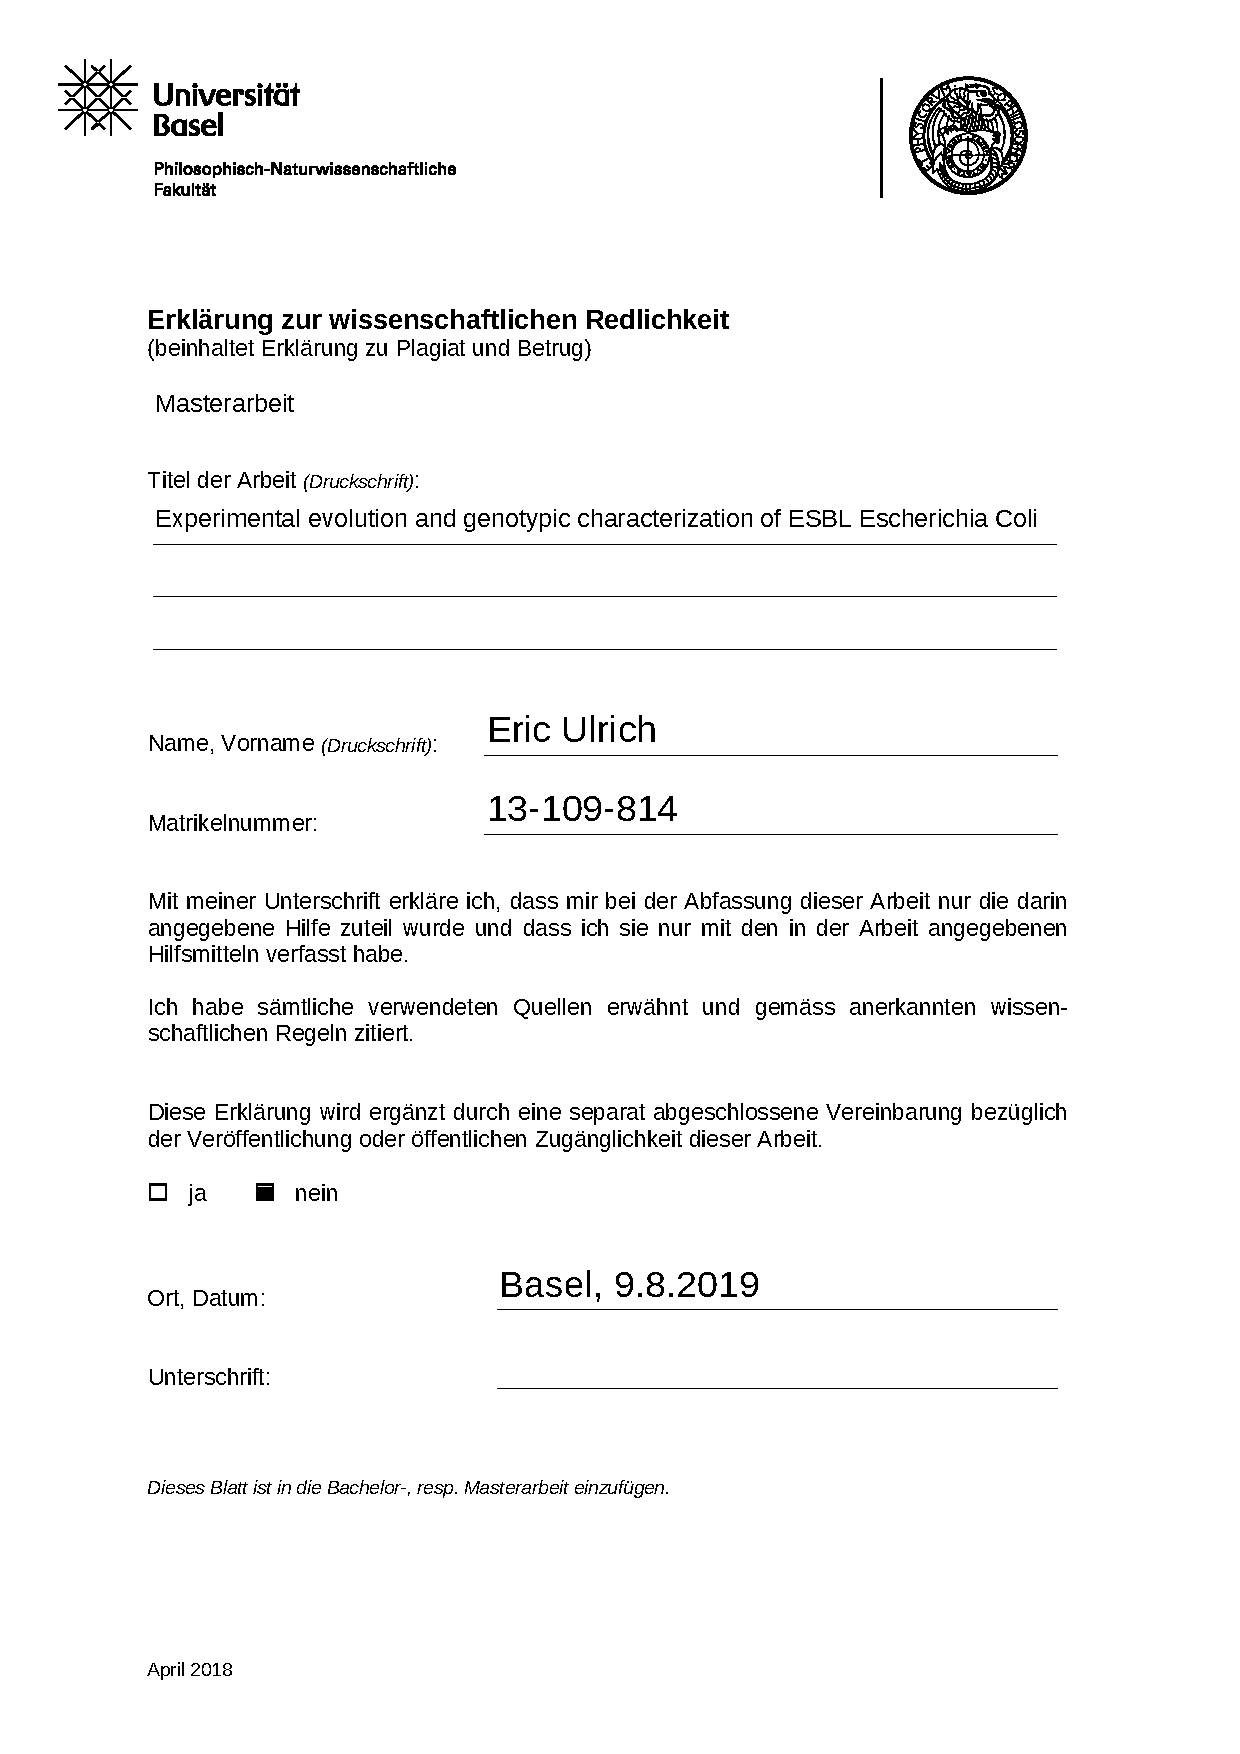
\includepdf[pages=-]{/home/ericulrich/masterarbeit/LaTeX_thesis/Declaration/Images/dec_edited.pdf}
\end{document}
